% !TEX root = presentation.tex
\section{Empirical Evaluation}
\subsection{Test Subjects}
\frame{\frametitle{Test Subjects}
  \tiny
  \rowcolors{2}{gray!30}{gray!20}
  \begin{tabular}{|l|>{\raggedleft\arraybackslash}p{0.8cm}|>{\raggedleft\arraybackslash}p{0.8cm}|>{\raggedleft\arraybackslash}p{0.9cm}|>{\raggedleft\arraybackslash}p{0.8cm}|>{\raggedleft\arraybackslash}p{0.8cm}|>{\raggedleft\arraybackslash}p{0.9cm}|>{\raggedleft\arraybackslash}p{0.8cm}|}
    \hline
    \rowcolor[RGB]{169,196,223}
    \textbf{Test Subject} & \textbf{Source LOC\footnotemark} & \textbf{Source Classes} & \textbf{Source Methods} & \textbf{Test LOC} & \textbf{Test Classes} & \textbf{Test Methods} & \textbf{Test Cases} \\
    \hline \emph{logback-core} & 12118 & 249 & 1270 & 8377 & 174 & 688 & 286 \\
    \hline \emph{barbecue} & 4790 & 58 & 299 & 2910 & 38 & 416 & 225 \\
    \hline \emph{jgap } & 28975 & 415 & 3017 & 19694 & 180 & 1633 & 1355 \\
    \hline \emph{commons-lang} & 19499 & 149 & 1196 & 33332 & 242 & 2408 & 2050 \\
    \hline \emph{joda-time} & 27139 & 227 & 3635 & 51388 & 221 & 4755 & 3866 \\
    \hline \emph{openfast} & 11646 & 265 & 1447 & 5587 & 115 & 421 & 322 \\
    \hline \emph{jsoup} & 10949 & 198 & 954 & 2883 & 25 & 335 & 319 \\
    \hline \emph{joda-primitives} & 11157 & 128 & 1868 & 6989 & 49 & 746 & 1810 \\
    \hline \textbf{all} & \textbf{126273} & \textbf{1689} & \textbf{13686} & \textbf{131160} & \textbf{1044} & \textbf{11402} & \textbf{10233} \\
    \hline
  \end{tabular}
  \footnotetext{Lines of Code (LOC)}
}

\subsubsection{Test Subjects [cont.]}
\frame{\frametitle{Test Subjects [cont.]}
  \begin{itemize}
    \item We use all subjects individually (\textit{subject})
    \item We use all subjects collectively (\textit{all})
    \item We use all subjects except one (\textit{all\_but\_subject})
  \end{itemize}
}

\subsection{Experiments}
\frame{\frametitle{Experiments}
  \begin{enumerate}
    \item \textbf{Mutation Score Distribution}: Identify classification categories.
     \item \textbf{Cross-Validation}: Acquire cross-validation accuracy using the different feature sets.
    \item \textbf{Prediction on Unknown Data}: Simulate realistic prediction on unknown data.
    \item \textbf{Optimization and Generalization}: Identify the most appropriate parameters that generalize to unknown data prediction.
    \item \textbf{Impact of Training Data Availability on Prediction Accuracy}: Evaluate the applicability of the approach in iterative development.
  \end{enumerate}
}

\subsubsection{Mutation Testing Results}
\frame{\frametitle{Mutation Testing Results}
  \tiny
  \rowcolors{2}{gray!30}{gray!20}
  \begin{tabular}{|l|>{\raggedleft}p{1.0cm}|>{\raggedleft}p{1.0cm}|>{\raggedleft}p{1.0cm}|>{\raggedleft}p{1.0cm}|>{\raggedleft}p{1.0cm}|>{\raggedleft\arraybackslash}p{1.2cm}|}
    \rowcolor[RGB]{169,196,223}
    \hline \textbf{Test Subject} & \textbf{Mutants Generated} & \textbf{Mutants Covered} & \textbf{Coverage (\%)} & \textbf{Mutants Killed} & \textbf{Mutation Score (\%)} & \textbf{Time Taken (\emph{hh:mm:ss})} \\
    \hline \emph{logback-core} & 10682 & 7350 & 68.8073 & 5400 & 73.4694 & 01:49:10 \\
    \hline \emph{barbecue} & 27324 & 4339 & 15.8798 & 2727 & 62.8486 & 00:49:51 \\
    \hline \emph{jgap} & 31929 & 17903 & 56.0713 & 13328 & 74.4456 & 07:04:44 \\
    \hline \emph{commons-lang} & 45141 & 41761 & 92.5124 & 33772 & 80.8697 & 15:51:59 \\
    \hline \emph{joda-time} & 70594 & 58595 & 83.0028 & 48545 & 82.8484 & 31:55:50 \\
    \hline \emph{openfast} & 14910 & 8371 & 56.1435 & 6869 & 82.0571 & 01:34:38 \\
    \hline \emph{jsoup} & 14165 & 10540 & 74.4088 & 8430 & 79.9810 & 03:55:56 \\
    \hline \emph{joda-primitives} & 22269 & 17334 & 77.8391 & 13499 & 77.8759 & 01:24:33 \\
    \hline \textbf{all} & \textbf{237014} & \textbf{166193} & \textbf{70.1195} & \textbf{132570} & \textbf{79.7687} & \textbf{64:26:41} \\
    \hline
  \end{tabular}
}

\subsection{Mutation Score Distribution}
\frame{\frametitle{Mutation Score Distribution}
  \begin{figure}[!tb]
    \centering
    \begin{tikzpicture}
    \begin{axis}[
        bar width=1,
        ymajorgrids=true,
        xlabel=Mutation Score (\%),
        ylabel=\# of Methods,
        width=\linewidth,
        height=6.0cm]
        \addplot[ybar,fill=black] file {../thesis/plots/all/evaluation_projects_method_distribution.txt};
    \end{axis}
    \end{tikzpicture}
    \caption{Mutation score distribution of methods from all eight test subjects that can be used for training.}
    \label{fig:mutation_distributions_method_all}
  \end{figure}
}

\subsubsection{Mutation Score Categories}
\frame{\frametitle{Mutation Score Categories}
\begin{table}[!tb]
    \scriptsize
    \centering
    \rowcolors{2}{gray!30}{gray!20}
    \begin{tabular}{|l|>{\raggedleft\arraybackslash}p{2cm}|>{\raggedleft\arraybackslash}p{2cm}|>{\raggedleft\arraybackslash}p{2cm}|}
      \hline
      \rowcolor[RGB]{169,196,223}
      \textbf{Category} & \textbf{Mutation Score Range} & \textbf{Class-Level} & \textbf{Method-Level} \\
      \hline LOW & [0\% -- 70\%) & 191 & 1104 \\
      \hline MEDIUM & [70\% -- 90\%) & 459 & 1782 \\
      \hline HIGH & [90\% -- 100\%] & 214 & 2624 \\
      \hline
    \end{tabular}
    \caption{The available number of source code units that fall within the determined ranges of mutation scores.}
    \label{tab:available_data}
  \end{table}
}

\subsection{Feature Sets}
\frame{\frametitle{Feature Sets}
  \begin{itemize}
    \item 33 individual metrics logically grouped into four feature sets:
    \begin{itemize}
      \item \ding{172} -- Source Code.
      \item \ding{173} -- Coverage.
      \item \ding{174} -- Accumulated Source Code.
      \item \ding{175} -- Accumulated Test Case.
    \end{itemize}
  \end{itemize}
}

\subsubsection{Evaluating Feature Sets}
\frame{\frametitle{Evaluating Feature Sets}
  \begin{figure}[!tb]
    \centering
    \begin{adjustbox}{max size={.95\textwidth}{.95\textheight}}
      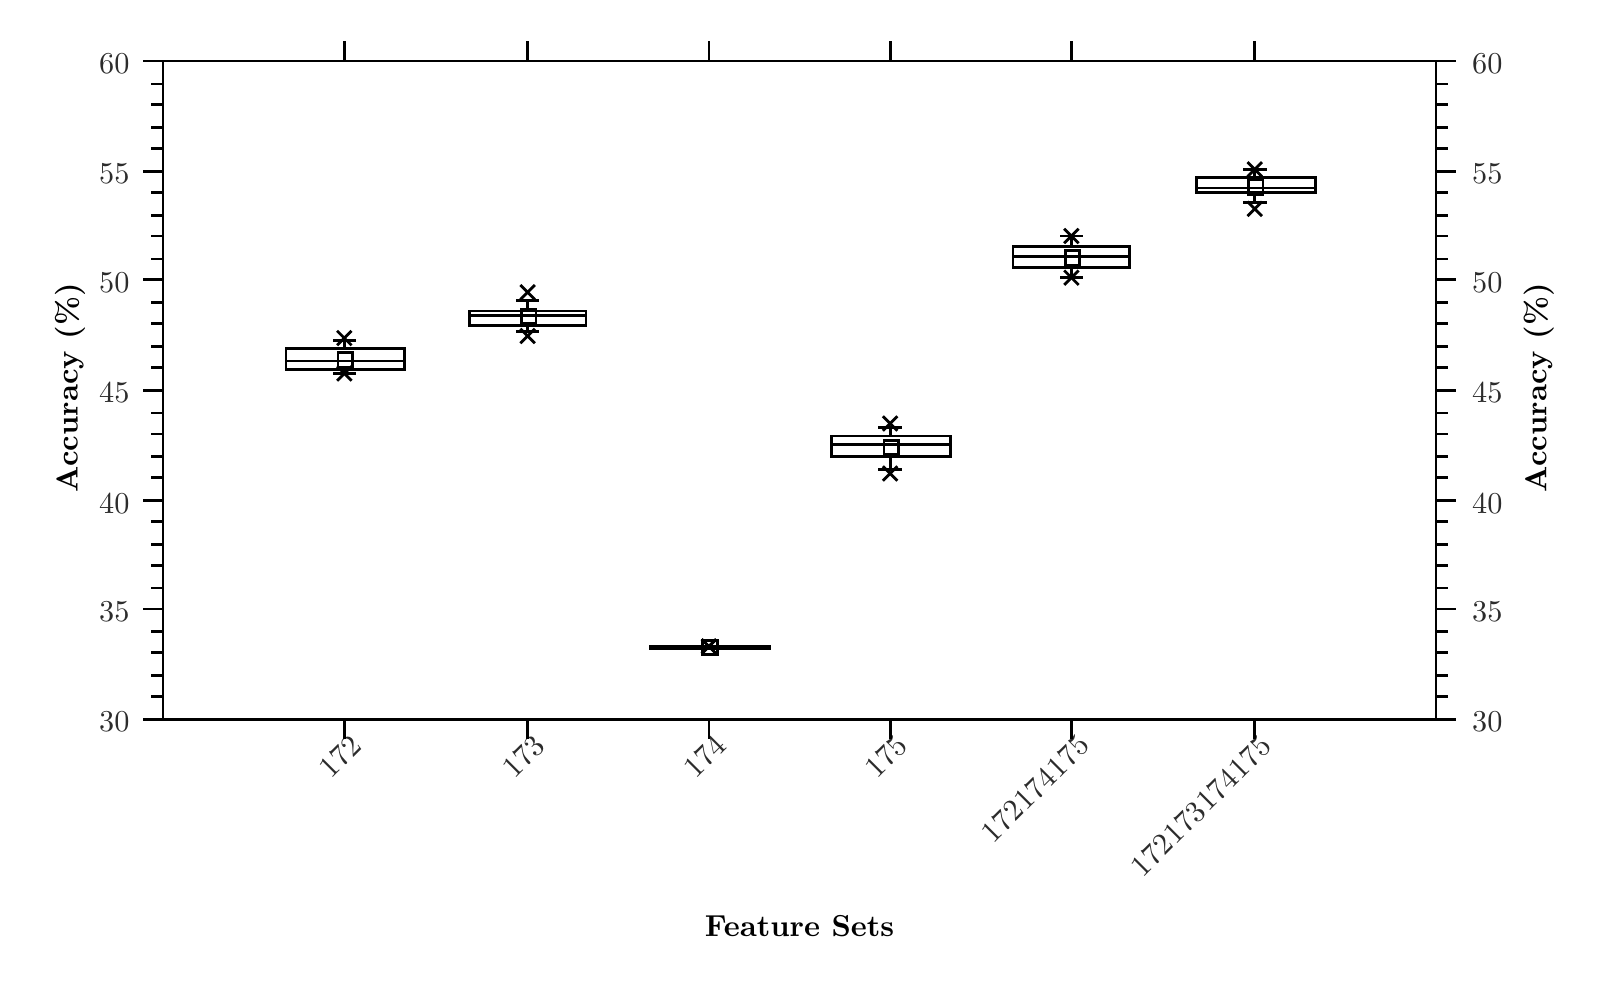
\begin{tikzpicture}{0pt}{0pt}{742pt}{452pt}
	\clip(0pt,452pt) -- (558.587pt,452pt) -- (558.587pt,111.729pt) -- (0pt,111.729pt) -- (0pt,452pt);
\begin{scope}
	\clip(48.9328pt,439.955pt) -- (508.901pt,439.955pt) -- (508.901pt,202.066pt) -- (48.9328pt,202.066pt) -- (48.9328pt,439.955pt);
	\color[rgb]{0,0,0}
	\draw[line width=1pt, line join=miter, line cap=rect](93.3487pt,336.067pt) -- (136.259pt,336.067pt) -- (136.259pt,328.539pt) -- (93.3487pt,328.539pt) -- (93.3487pt,336.067pt);
	\color[rgb]{0,0,0}
	\draw[line width=1pt, line join=miter, line cap=rect](110.663pt,327.033pt) -- (118.192pt,327.033pt);
	\draw[line width=1pt, line join=miter, line cap=rect](110.663pt,339.078pt) -- (118.192pt,339.078pt);
	\draw[line width=1pt, line join=miter, line cap=rect](114.427pt,339.078pt) -- (114.427pt,336.067pt);
	\draw[line width=1pt, line join=miter, line cap=rect](114.427pt,327.033pt) -- (114.427pt,328.539pt);
	\draw[line width=1pt, line join=miter, line cap=rect](93.3487pt,331.55pt) -- (135.506pt,331.55pt);
	\draw[line width=1pt, line join=miter, line cap=rect](112.169pt,329.292pt) -- (116.686pt,324.775pt);
	\draw[line width=1pt, line join=miter, line cap=rect](112.169pt,324.775pt) -- (116.686pt,329.292pt);
	\draw[line width=1pt, line join=miter, line cap=rect](112.169pt,342.089pt) -- (116.686pt,337.572pt);
	\draw[line width=1pt, line join=miter, line cap=rect](112.169pt,337.572pt) -- (116.686pt,342.089pt);
	\draw[line width=1pt, line join=miter, line cap=rect](112.169pt,334.561pt) -- (117.439pt,334.561pt) -- (117.439pt,329.292pt) -- (112.169pt,329.292pt) -- (112.169pt,334.561pt);
	\draw[line width=1pt, line join=miter, line cap=rect](159.596pt,349.618pt) -- (201.754pt,349.618pt) -- (201.754pt,344.348pt) -- (159.596pt,344.348pt) -- (159.596pt,349.618pt);
	\draw[line width=1pt, line join=miter, line cap=rect](176.911pt,342.089pt) -- (184.439pt,342.089pt);
	\draw[line width=1pt, line join=miter, line cap=rect](176.911pt,353.382pt) -- (184.439pt,353.382pt);
	\draw[line width=1pt, line join=miter, line cap=rect](180.675pt,353.382pt) -- (180.675pt,349.618pt);
	\draw[line width=1pt, line join=miter, line cap=rect](180.675pt,342.089pt) -- (180.675pt,344.348pt);
	\draw[line width=1pt, line join=miter, line cap=rect](159.596pt,348.112pt) -- (201.754pt,348.112pt);
	\draw[line width=1pt, line join=miter, line cap=rect](178.417pt,342.842pt) -- (182.933pt,338.325pt);
	\draw[line width=1pt, line join=miter, line cap=rect](178.417pt,338.325pt) -- (182.933pt,342.842pt);
	\draw[line width=1pt, line join=miter, line cap=rect](178.417pt,358.651pt) -- (182.933pt,354.134pt);
	\draw[line width=1pt, line join=miter, line cap=rect](178.417pt,354.134pt) -- (182.933pt,358.651pt);
	\draw[line width=1pt, line join=miter, line cap=rect](178.417pt,350.37pt) -- (183.686pt,350.37pt) -- (183.686pt,345.101pt) -- (178.417pt,345.101pt) -- (178.417pt,350.37pt);
	\draw[line width=1pt, line join=miter, line cap=rect](225.091pt,228.415pt) -- (268.001pt,228.415pt) -- (268.001pt,227.662pt) -- (225.091pt,227.662pt) -- (225.091pt,228.415pt);
	\draw[line width=1pt, line join=miter, line cap=rect](242.406pt,228.415pt) -- (249.934pt,228.415pt);
	\draw[line width=1pt, line join=miter, line cap=rect](242.406pt,228.415pt) -- (249.934pt,228.415pt);
	\draw[line width=1pt, line join=miter, line cap=rect](225.091pt,228.415pt) -- (267.248pt,228.415pt);
	\draw[line width=1pt, line join=miter, line cap=rect](243.911pt,230.673pt) -- (248.428pt,226.156pt);
	\draw[line width=1pt, line join=miter, line cap=rect](243.911pt,226.156pt) -- (248.428pt,230.673pt);
	\draw[line width=1pt, line join=miter, line cap=rect](243.911pt,230.673pt) -- (248.428pt,226.156pt);
	\draw[line width=1pt, line join=miter, line cap=rect](243.911pt,226.156pt) -- (248.428pt,230.673pt);
	\draw[line width=1pt, line join=miter, line cap=rect](243.911pt,230.673pt) -- (249.181pt,230.673pt) -- (249.181pt,225.403pt) -- (243.911pt,225.403pt) -- (243.911pt,230.673pt);
	\draw[line width=1pt, line join=miter, line cap=rect](290.586pt,304.449pt) -- (333.496pt,304.449pt) -- (333.496pt,296.921pt) -- (290.586pt,296.921pt) -- (290.586pt,304.449pt);
	\draw[line width=1pt, line join=miter, line cap=rect](307.9pt,292.404pt) -- (315.428pt,292.404pt);
	\draw[line width=1pt, line join=miter, line cap=rect](307.9pt,307.46pt) -- (315.428pt,307.46pt);
	\draw[line width=1pt, line join=miter, line cap=rect](311.664pt,307.46pt) -- (311.664pt,304.449pt);
	\draw[line width=1pt, line join=miter, line cap=rect](311.664pt,292.404pt) -- (311.664pt,296.921pt);
	\draw[line width=1pt, line join=miter, line cap=rect](290.586pt,301.438pt) -- (332.743pt,301.438pt);
	\draw[line width=1pt, line join=miter, line cap=rect](309.406pt,293.157pt) -- (313.923pt,288.64pt);
	\draw[line width=1pt, line join=miter, line cap=rect](309.406pt,288.64pt) -- (313.923pt,293.157pt);
	\draw[line width=1pt, line join=miter, line cap=rect](309.406pt,311.224pt) -- (313.923pt,306.707pt);
	\draw[line width=1pt, line join=miter, line cap=rect](309.406pt,306.707pt) -- (313.923pt,311.224pt);
	\draw[line width=1pt, line join=miter, line cap=rect](309.406pt,302.943pt) -- (314.676pt,302.943pt) -- (314.676pt,297.673pt) -- (309.406pt,297.673pt) -- (309.406pt,302.943pt);
	\draw[line width=1pt, line join=miter, line cap=rect](356.08pt,372.955pt) -- (398.238pt,372.955pt) -- (398.238pt,365.427pt) -- (356.08pt,365.427pt) -- (356.08pt,372.955pt);
	\draw[line width=1pt, line join=miter, line cap=rect](373.395pt,361.663pt) -- (380.923pt,361.663pt);
	\draw[line width=1pt, line join=miter, line cap=rect](373.395pt,376.719pt) -- (380.923pt,376.719pt);
	\draw[line width=1pt, line join=miter, line cap=rect](377.159pt,376.719pt) -- (377.159pt,372.955pt);
	\draw[line width=1pt, line join=miter, line cap=rect](377.159pt,361.663pt) -- (377.159pt,365.427pt);
	\draw[line width=1pt, line join=miter, line cap=rect](356.08pt,369.191pt) -- (398.238pt,369.191pt);
	\draw[line width=1pt, line join=miter, line cap=rect](374.901pt,363.921pt) -- (379.418pt,359.404pt);
	\draw[line width=1pt, line join=miter, line cap=rect](374.901pt,359.404pt) -- (379.418pt,363.921pt);
	\draw[line width=1pt, line join=miter, line cap=rect](374.901pt,378.977pt) -- (379.418pt,374.46pt);
	\draw[line width=1pt, line join=miter, line cap=rect](374.901pt,374.46pt) -- (379.418pt,378.977pt);
	\draw[line width=1pt, line join=miter, line cap=rect](374.901pt,371.449pt) -- (380.17pt,371.449pt) -- (380.17pt,366.179pt) -- (374.901pt,366.179pt) -- (374.901pt,371.449pt);
	\draw[line width=1pt, line join=miter, line cap=rect](422.328pt,397.798pt) -- (465.238pt,397.798pt) -- (465.238pt,392.528pt) -- (422.328pt,392.528pt) -- (422.328pt,397.798pt);
	\draw[line width=1pt, line join=miter, line cap=rect](439.642pt,388.764pt) -- (447.171pt,388.764pt);
	\draw[line width=1pt, line join=miter, line cap=rect](439.642pt,400.809pt) -- (447.171pt,400.809pt);
	\draw[line width=1pt, line join=miter, line cap=rect](443.407pt,400.809pt) -- (443.407pt,397.798pt);
	\draw[line width=1pt, line join=miter, line cap=rect](443.407pt,388.764pt) -- (443.407pt,392.528pt);
	\draw[line width=1pt, line join=miter, line cap=rect](422.328pt,394.033pt) -- (464.485pt,394.033pt);
	\draw[line width=1pt, line join=miter, line cap=rect](441.148pt,388.764pt) -- (445.665pt,384.247pt);
	\draw[line width=1pt, line join=miter, line cap=rect](441.148pt,384.247pt) -- (445.665pt,388.764pt);
	\draw[line width=1pt, line join=miter, line cap=rect](441.148pt,403.067pt) -- (445.665pt,398.55pt);
	\draw[line width=1pt, line join=miter, line cap=rect](441.148pt,398.55pt) -- (445.665pt,403.067pt);
	\draw[line width=1pt, line join=miter, line cap=rect](441.148pt,397.045pt) -- (446.418pt,397.045pt) -- (446.418pt,391.775pt) -- (441.148pt,391.775pt) -- (441.148pt,397.045pt);
\end{scope}
\begin{scope}
	\color[rgb]{0,0,0}
	\pgftext[center, base, at={\pgfpoint{18.0675pt}{321.763pt}},rotate=90]{\fontsize{11}{0}\selectfont{\textbf{Accuracy (\%)}}}
	\color[rgb]{0.172549,0.172549,0.172549}
	\pgftext[center, base, at={\pgfpoint{31.3358pt}{197.549pt}}]{\fontsize{11}{0}\selectfont{30}}
	\pgftext[center, base, at={\pgfpoint{31.3358pt}{237.448pt}}]{\fontsize{11}{0}\selectfont{35}}
	\pgftext[center, base, at={\pgfpoint{31.3358pt}{276.595pt}}]{\fontsize{11}{0}\selectfont{40}}
	\pgftext[center, base, at={\pgfpoint{31.3358pt}{316.494pt}}]{\fontsize{11}{0}\selectfont{45}}
	\pgftext[center, base, at={\pgfpoint{31.3358pt}{356.393pt}}]{\fontsize{11}{0}\selectfont{50}}
	\pgftext[center, base, at={\pgfpoint{31.3358pt}{395.539pt}}]{\fontsize{11}{0}\selectfont{55}}
	\pgftext[center, base, at={\pgfpoint{31.3358pt}{435.438pt}}]{\fontsize{11}{0}\selectfont{60}}
	\color[rgb]{0,0,0}
	\draw[line width=1pt, line join=bevel, line cap=rect](48.9328pt,210.347pt) -- (45.1688pt,210.347pt);
	\draw[line width=1pt, line join=bevel, line cap=rect](48.9328pt,217.875pt) -- (45.1688pt,217.875pt);
	\draw[line width=1pt, line join=bevel, line cap=rect](48.9328pt,226.156pt) -- (45.1688pt,226.156pt);
	\draw[line width=1pt, line join=bevel, line cap=rect](48.9328pt,233.684pt) -- (45.1688pt,233.684pt);
	\draw[line width=1pt, line join=bevel, line cap=rect](48.9328pt,249.493pt) -- (45.1688pt,249.493pt);
	\draw[line width=1pt, line join=bevel, line cap=rect](48.9328pt,257.774pt) -- (45.1688pt,257.774pt);
	\draw[line width=1pt, line join=bevel, line cap=rect](48.9328pt,265.303pt) -- (45.1688pt,265.303pt);
	\draw[line width=1pt, line join=bevel, line cap=rect](48.9328pt,273.583pt) -- (45.1688pt,273.583pt);
	\draw[line width=1pt, line join=bevel, line cap=rect](48.9328pt,289.393pt) -- (45.1688pt,289.393pt);
	\draw[line width=1pt, line join=bevel, line cap=rect](48.9328pt,296.921pt) -- (45.1688pt,296.921pt);
	\draw[line width=1pt, line join=bevel, line cap=rect](48.9328pt,305.202pt) -- (45.1688pt,305.202pt);
	\draw[line width=1pt, line join=bevel, line cap=rect](48.9328pt,312.73pt) -- (45.1688pt,312.73pt);
	\draw[line width=1pt, line join=bevel, line cap=rect](48.9328pt,329.292pt) -- (45.1688pt,329.292pt);
	\draw[line width=1pt, line join=bevel, line cap=rect](48.9328pt,336.82pt) -- (45.1688pt,336.82pt);
	\draw[line width=1pt, line join=bevel, line cap=rect](48.9328pt,345.101pt) -- (45.1688pt,345.101pt);
	\draw[line width=1pt, line join=bevel, line cap=rect](48.9328pt,352.629pt) -- (45.1688pt,352.629pt);
	\draw[line width=1pt, line join=bevel, line cap=rect](48.9328pt,368.438pt) -- (45.1688pt,368.438pt);
	\draw[line width=1pt, line join=bevel, line cap=rect](48.9328pt,376.719pt) -- (45.1688pt,376.719pt);
	\draw[line width=1pt, line join=bevel, line cap=rect](48.9328pt,384.247pt) -- (45.1688pt,384.247pt);
	\draw[line width=1pt, line join=bevel, line cap=rect](48.9328pt,392.528pt) -- (45.1688pt,392.528pt);
	\draw[line width=1pt, line join=bevel, line cap=rect](48.9328pt,408.337pt) -- (45.1688pt,408.337pt);
	\draw[line width=1pt, line join=bevel, line cap=rect](48.9328pt,415.865pt) -- (45.1688pt,415.865pt);
	\draw[line width=1pt, line join=bevel, line cap=rect](48.9328pt,424.146pt) -- (45.1688pt,424.146pt);
	\draw[line width=1pt, line join=bevel, line cap=rect](48.9328pt,431.674pt) -- (45.1688pt,431.674pt);
	\draw[line width=1pt, line join=bevel, line cap=rect](48.9328pt,202.066pt) -- (42.1575pt,202.066pt);
	\draw[line width=1pt, line join=bevel, line cap=rect](48.9328pt,241.965pt) -- (42.1575pt,241.965pt);
	\draw[line width=1pt, line join=bevel, line cap=rect](48.9328pt,281.112pt) -- (42.1575pt,281.112pt);
	\draw[line width=1pt, line join=bevel, line cap=rect](48.9328pt,321.011pt) -- (42.1575pt,321.011pt);
	\draw[line width=1pt, line join=bevel, line cap=rect](48.9328pt,360.91pt) -- (42.1575pt,360.91pt);
	\draw[line width=1pt, line join=bevel, line cap=rect](48.9328pt,400.056pt) -- (42.1575pt,400.056pt);
	\draw[line width=1pt, line join=bevel, line cap=rect](48.9328pt,439.955pt) -- (42.1575pt,439.955pt);
	\draw[line width=1pt, line join=bevel, line cap=rect](48.9328pt,439.955pt) -- (48.9328pt,202.066pt);
	\pgftext[center, base, at={\pgfpoint{548.8pt}{321.763pt}},rotate=90]{\fontsize{11}{0}\selectfont{\textbf{Accuracy (\%)}}}
	\color[rgb]{0.172549,0.172549,0.172549}
	\pgftext[center, base, at={\pgfpoint{527.439pt}{197.549pt}}]{\fontsize{11}{0}\selectfont{30}}
	\pgftext[center, base, at={\pgfpoint{527.439pt}{237.448pt}}]{\fontsize{11}{0}\selectfont{35}}
	\pgftext[center, base, at={\pgfpoint{527.439pt}{276.595pt}}]{\fontsize{11}{0}\selectfont{40}}
	\pgftext[center, base, at={\pgfpoint{527.439pt}{316.494pt}}]{\fontsize{11}{0}\selectfont{45}}
	\pgftext[center, base, at={\pgfpoint{527.439pt}{356.393pt}}]{\fontsize{11}{0}\selectfont{50}}
	\pgftext[center, base, at={\pgfpoint{527.439pt}{395.539pt}}]{\fontsize{11}{0}\selectfont{55}}
	\pgftext[center, base, at={\pgfpoint{527.439pt}{435.438pt}}]{\fontsize{11}{0}\selectfont{60}}
	\color[rgb]{0,0,0}
	\draw[line width=1pt, line join=bevel, line cap=rect](508.901pt,210.347pt) -- (512.665pt,210.347pt);
	\draw[line width=1pt, line join=bevel, line cap=rect](508.901pt,217.875pt) -- (512.665pt,217.875pt);
	\draw[line width=1pt, line join=bevel, line cap=rect](508.901pt,226.156pt) -- (512.665pt,226.156pt);
	\draw[line width=1pt, line join=bevel, line cap=rect](508.901pt,233.684pt) -- (512.665pt,233.684pt);
	\draw[line width=1pt, line join=bevel, line cap=rect](508.901pt,249.493pt) -- (512.665pt,249.493pt);
	\draw[line width=1pt, line join=bevel, line cap=rect](508.901pt,257.774pt) -- (512.665pt,257.774pt);
	\draw[line width=1pt, line join=bevel, line cap=rect](508.901pt,265.303pt) -- (512.665pt,265.303pt);
	\draw[line width=1pt, line join=bevel, line cap=rect](508.901pt,273.583pt) -- (512.665pt,273.583pt);
	\draw[line width=1pt, line join=bevel, line cap=rect](508.901pt,289.393pt) -- (512.665pt,289.393pt);
	\draw[line width=1pt, line join=bevel, line cap=rect](508.901pt,296.921pt) -- (512.665pt,296.921pt);
	\draw[line width=1pt, line join=bevel, line cap=rect](508.901pt,305.202pt) -- (512.665pt,305.202pt);
	\draw[line width=1pt, line join=bevel, line cap=rect](508.901pt,312.73pt) -- (512.665pt,312.73pt);
	\draw[line width=1pt, line join=bevel, line cap=rect](508.901pt,329.292pt) -- (512.665pt,329.292pt);
	\draw[line width=1pt, line join=bevel, line cap=rect](508.901pt,336.82pt) -- (512.665pt,336.82pt);
	\draw[line width=1pt, line join=bevel, line cap=rect](508.901pt,345.101pt) -- (512.665pt,345.101pt);
	\draw[line width=1pt, line join=bevel, line cap=rect](508.901pt,352.629pt) -- (512.665pt,352.629pt);
	\draw[line width=1pt, line join=bevel, line cap=rect](508.901pt,368.438pt) -- (512.665pt,368.438pt);
	\draw[line width=1pt, line join=bevel, line cap=rect](508.901pt,376.719pt) -- (512.665pt,376.719pt);
	\draw[line width=1pt, line join=bevel, line cap=rect](508.901pt,384.247pt) -- (512.665pt,384.247pt);
	\draw[line width=1pt, line join=bevel, line cap=rect](508.901pt,392.528pt) -- (512.665pt,392.528pt);
	\draw[line width=1pt, line join=bevel, line cap=rect](508.901pt,408.337pt) -- (512.665pt,408.337pt);
	\draw[line width=1pt, line join=bevel, line cap=rect](508.901pt,415.865pt) -- (512.665pt,415.865pt);
	\draw[line width=1pt, line join=bevel, line cap=rect](508.901pt,424.146pt) -- (512.665pt,424.146pt);
	\draw[line width=1pt, line join=bevel, line cap=rect](508.901pt,431.674pt) -- (512.665pt,431.674pt);
	\draw[line width=1pt, line join=bevel, line cap=rect](508.901pt,202.066pt) -- (515.677pt,202.066pt);
	\draw[line width=1pt, line join=bevel, line cap=rect](508.901pt,241.965pt) -- (515.677pt,241.965pt);
	\draw[line width=1pt, line join=bevel, line cap=rect](508.901pt,281.112pt) -- (515.677pt,281.112pt);
	\draw[line width=1pt, line join=bevel, line cap=rect](508.901pt,321.011pt) -- (515.677pt,321.011pt);
	\draw[line width=1pt, line join=bevel, line cap=rect](508.901pt,360.91pt) -- (515.677pt,360.91pt);
	\draw[line width=1pt, line join=bevel, line cap=rect](508.901pt,400.056pt) -- (515.677pt,400.056pt);
	\draw[line width=1pt, line join=bevel, line cap=rect](508.901pt,439.955pt) -- (515.677pt,439.955pt);
	\draw[line width=1pt, line join=bevel, line cap=rect](508.901pt,439.955pt) -- (508.901pt,202.066pt);
	\pgftext[center, base, at={\pgfpoint{278.911pt}{123.774pt}}]{\fontsize{11}{0}\selectfont{\textbf{Feature Sets}}}
	\color[rgb]{0.172549,0.172549,0.172549}
	\pgftext[center, base, at={\pgfpoint{115.392pt}{186.104pt}},rotate=45]{\fontsize{11}{0}\selectfont{\ding{172}}}
	\pgftext[center, base, at={\pgfpoint{181.64pt}{186.104pt}},rotate=45]{\fontsize{11}{0}\selectfont{\ding{173}}}
	\pgftext[center, base, at={\pgfpoint{247.135pt}{186.104pt}},rotate=45]{\fontsize{11}{0}\selectfont{\ding{174}}}
	\pgftext[center, base, at={\pgfpoint{312.629pt}{186.104pt}},rotate=45]{\fontsize{11}{0}\selectfont{\ding{175}}}
	\pgftext[center, base, at={\pgfpoint{354.702pt}{162.682pt}},rotate=45]{\fontsize{11}{0}\selectfont{\ding{172}}}
	\pgftext[center, base, at={\pgfpoint{366.513pt}{174.493pt}},rotate=45]{\fontsize{11}{0}\selectfont{\ding{174}}}
	\pgftext[center, base, at={\pgfpoint{378.324pt}{186.303pt}},rotate=45]{\fontsize{11}{0}\selectfont{\ding{175}}}
	\pgftext[center, base, at={\pgfpoint{408.706pt}{150.439pt}},rotate=45]{\fontsize{11}{0}\selectfont{\ding{172}}}
	\pgftext[center, base, at={\pgfpoint{420.517pt}{162.249pt}},rotate=45]{\fontsize{11}{0}\selectfont{\ding{173}}}
	\pgftext[center, base, at={\pgfpoint{432.328pt}{174.06pt}},rotate=45]{\fontsize{11}{0}\selectfont{\ding{174}}}
	\pgftext[center, base, at={\pgfpoint{444.139pt}{185.871pt}},rotate=45]{\fontsize{11}{0}\selectfont{\ding{175}}}
	\color[rgb]{0,0,0}
	\draw[line width=1pt, line join=bevel, line cap=rect](114.427pt,202.066pt) -- (114.427pt,195.291pt);
	\draw[line width=1pt, line join=bevel, line cap=rect](180.675pt,202.066pt) -- (180.675pt,195.291pt);
	\draw[line width=1pt, line join=bevel, line cap=rect](246.17pt,202.066pt) -- (246.17pt,195.291pt);
	\draw[line width=1pt, line join=bevel, line cap=rect](311.664pt,202.066pt) -- (311.664pt,195.291pt);
	\draw[line width=1pt, line join=bevel, line cap=rect](377.159pt,202.066pt) -- (377.159pt,195.291pt);
	\draw[line width=1pt, line join=bevel, line cap=rect](443.407pt,202.066pt) -- (443.407pt,195.291pt);
	\draw[line width=1pt, line join=bevel, line cap=rect](48.9328pt,202.066pt) -- (508.901pt,202.066pt);
	\draw[line width=1pt, line join=bevel, line cap=rect](114.427pt,439.955pt) -- (114.427pt,446.73pt);
	\draw[line width=1pt, line join=bevel, line cap=rect](180.675pt,439.955pt) -- (180.675pt,446.73pt);
	\draw[line width=1pt, line join=bevel, line cap=rect](246.17pt,439.955pt) -- (246.17pt,446.73pt);
	\draw[line width=1pt, line join=bevel, line cap=rect](311.664pt,439.955pt) -- (311.664pt,446.73pt);
	\draw[line width=1pt, line join=bevel, line cap=rect](377.159pt,439.955pt) -- (377.159pt,446.73pt);
	\draw[line width=1pt, line join=bevel, line cap=rect](443.407pt,439.955pt) -- (443.407pt,446.73pt);
	\draw[line width=1pt, line join=bevel, line cap=rect](48.9328pt,439.955pt) -- (508.901pt,439.955pt);
\end{scope}
\end{tikzpicture}

    \end{adjustbox}
    \caption{Method-level cross-validation accuracy of feature sets on the \textit{all} subject.}
    \label{fig:all_cross_validation_features_method_graph}
  \end{figure}
}

\subsubsection{Cross-Validation Accuracy}
\frame{\frametitle{Cross-Validation Accuracy}
  \begin{figure}[!tb]
    \centering
    \begin{adjustbox}{max size={.95\textwidth}{.95\textheight}}
      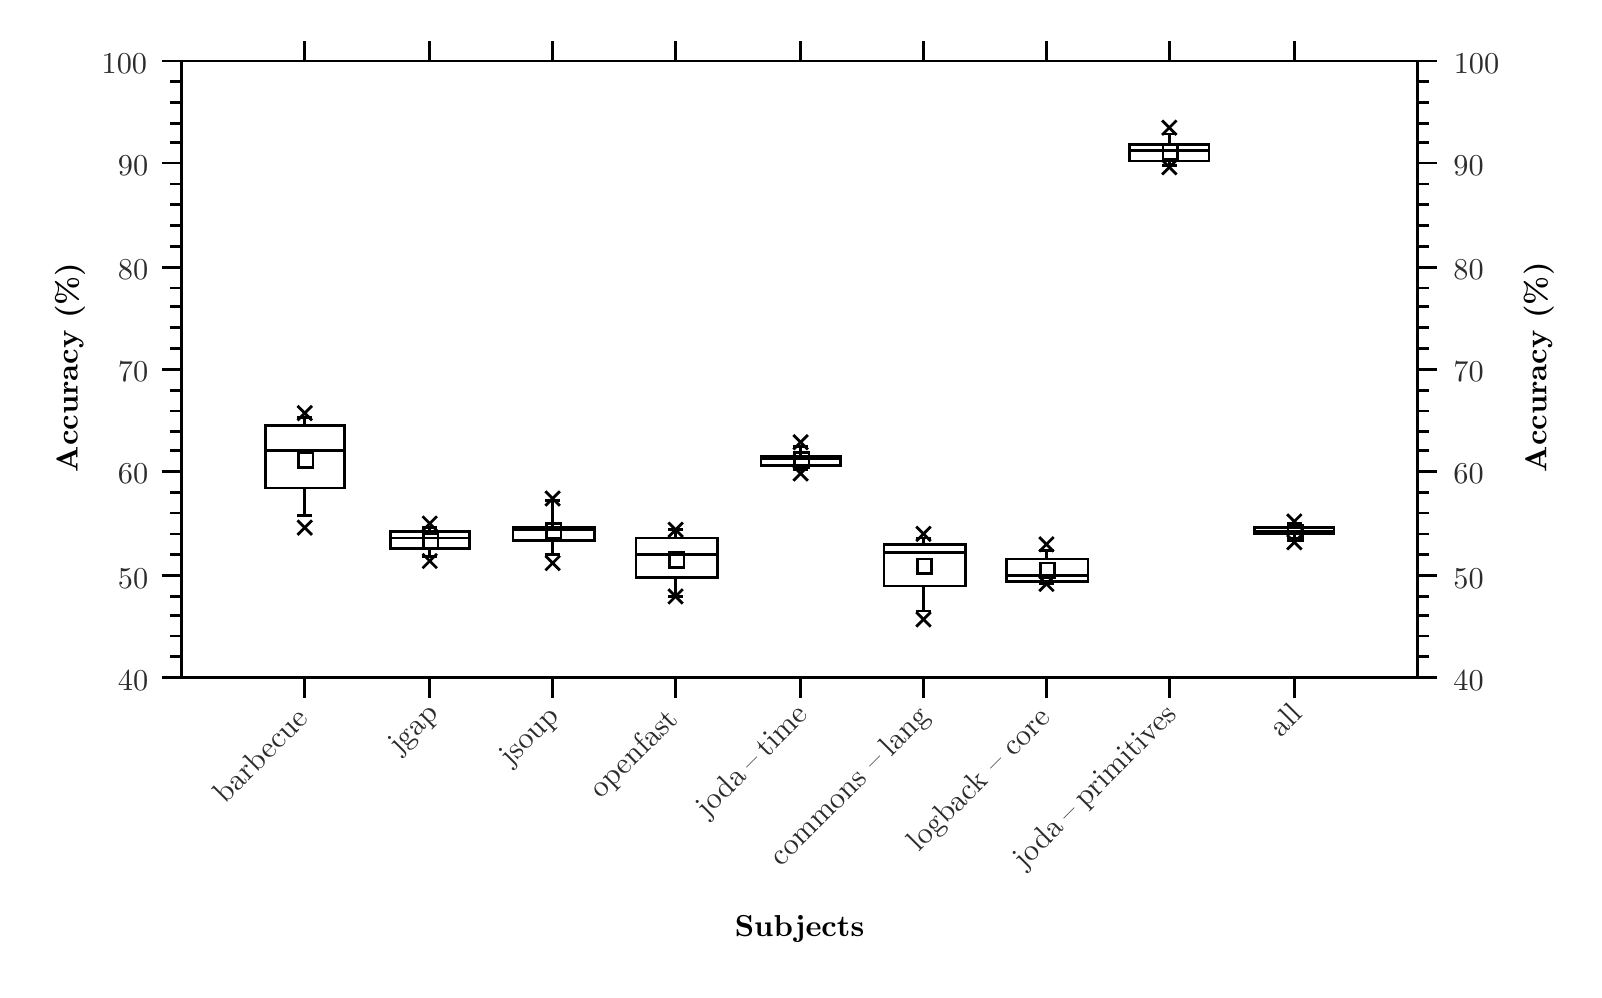
\begin{tikzpicture}{0pt}{0pt}{742pt}{452pt}
	\clip(0pt,452pt) -- (558.587pt,452pt) -- (558.587pt,111.729pt) -- (0pt,111.729pt) -- (0pt,452pt);
\begin{scope}
	\clip(55.7081pt,439.955pt) -- (502.126pt,439.955pt) -- (502.126pt,217.123pt) -- (55.7081pt,217.123pt) -- (55.7081pt,439.955pt);
	\color[rgb]{0,0,0}
	\draw[line width=1pt, line join=miter, line cap=rect](85.8206pt,308.213pt) -- (114.427pt,308.213pt) -- (114.427pt,285.628pt) -- (85.8206pt,285.628pt) -- (85.8206pt,308.213pt);
	\color[rgb]{0,0,0}
	\draw[line width=1pt, line join=miter, line cap=rect](97.8656pt,275.842pt) -- (102.382pt,275.842pt);
	\draw[line width=1pt, line join=miter, line cap=rect](97.8656pt,311.224pt) -- (102.382pt,311.224pt);
	\draw[line width=1pt, line join=miter, line cap=rect](100.124pt,311.224pt) -- (100.124pt,308.213pt);
	\draw[line width=1pt, line join=miter, line cap=rect](100.124pt,275.842pt) -- (100.124pt,285.628pt);
	\draw[line width=1pt, line join=miter, line cap=rect](85.8206pt,299.179pt) -- (114.427pt,299.179pt);
	\draw[line width=1pt, line join=miter, line cap=rect](97.8656pt,273.583pt) -- (102.382pt,269.067pt);
	\draw[line width=1pt, line join=miter, line cap=rect](97.8656pt,269.067pt) -- (102.382pt,273.583pt);
	\draw[line width=1pt, line join=miter, line cap=rect](97.8656pt,314.988pt) -- (102.382pt,310.471pt);
	\draw[line width=1pt, line join=miter, line cap=rect](97.8656pt,310.471pt) -- (102.382pt,314.988pt);
	\draw[line width=1pt, line join=miter, line cap=rect](97.8656pt,298.426pt) -- (103.135pt,298.426pt) -- (103.135pt,293.157pt) -- (97.8656pt,293.157pt) -- (97.8656pt,298.426pt);
	\draw[line width=1pt, line join=miter, line cap=rect](130.989pt,269.819pt) -- (159.596pt,269.819pt) -- (159.596pt,263.797pt) -- (130.989pt,263.797pt) -- (130.989pt,269.819pt);
	\draw[line width=1pt, line join=miter, line cap=rect](143.034pt,260.786pt) -- (147.551pt,260.786pt);
	\draw[line width=1pt, line join=miter, line cap=rect](143.034pt,271.325pt) -- (147.551pt,271.325pt);
	\draw[line width=1pt, line join=miter, line cap=rect](145.293pt,271.325pt) -- (145.293pt,269.819pt);
	\draw[line width=1pt, line join=miter, line cap=rect](145.293pt,260.786pt) -- (145.293pt,263.797pt);
	\draw[line width=1pt, line join=miter, line cap=rect](130.989pt,267.561pt) -- (159.596pt,267.561pt);
	\draw[line width=1pt, line join=miter, line cap=rect](143.034pt,261.538pt) -- (147.551pt,257.022pt);
	\draw[line width=1pt, line join=miter, line cap=rect](143.034pt,257.022pt) -- (147.551pt,261.538pt);
	\draw[line width=1pt, line join=miter, line cap=rect](143.034pt,275.089pt) -- (147.551pt,270.572pt);
	\draw[line width=1pt, line join=miter, line cap=rect](143.034pt,270.572pt) -- (147.551pt,275.089pt);
	\draw[line width=1pt, line join=miter, line cap=rect](143.034pt,269.067pt) -- (148.304pt,269.067pt) -- (148.304pt,263.797pt) -- (143.034pt,263.797pt) -- (143.034pt,269.067pt);
	\draw[line width=1pt, line join=miter, line cap=rect](175.405pt,271.325pt) -- (204.765pt,271.325pt) -- (204.765pt,266.808pt) -- (175.405pt,266.808pt) -- (175.405pt,271.325pt);
	\draw[line width=1pt, line join=miter, line cap=rect](187.45pt,261.538pt) -- (191.967pt,261.538pt);
	\draw[line width=1pt, line join=miter, line cap=rect](187.45pt,281.112pt) -- (191.967pt,281.112pt);
	\draw[line width=1pt, line join=miter, line cap=rect](189.709pt,281.112pt) -- (189.709pt,271.325pt);
	\draw[line width=1pt, line join=miter, line cap=rect](189.709pt,261.538pt) -- (189.709pt,266.808pt);
	\draw[line width=1pt, line join=miter, line cap=rect](175.405pt,270.572pt) -- (204.012pt,270.572pt);
	\draw[line width=1pt, line join=miter, line cap=rect](187.45pt,260.786pt) -- (191.967pt,256.269pt);
	\draw[line width=1pt, line join=miter, line cap=rect](187.45pt,256.269pt) -- (191.967pt,260.786pt);
	\draw[line width=1pt, line join=miter, line cap=rect](187.45pt,284.123pt) -- (191.967pt,279.606pt);
	\draw[line width=1pt, line join=miter, line cap=rect](187.45pt,279.606pt) -- (191.967pt,284.123pt);
	\draw[line width=1pt, line join=miter, line cap=rect](187.45pt,272.831pt) -- (192.72pt,272.831pt) -- (192.72pt,267.561pt) -- (187.45pt,267.561pt) -- (187.45pt,272.831pt);
	\draw[line width=1pt, line join=miter, line cap=rect](219.821pt,267.561pt) -- (249.181pt,267.561pt) -- (249.181pt,253.257pt) -- (219.821pt,253.257pt) -- (219.821pt,267.561pt);
	\draw[line width=1pt, line join=miter, line cap=rect](231.866pt,246.482pt) -- (236.383pt,246.482pt);
	\draw[line width=1pt, line join=miter, line cap=rect](231.866pt,270.572pt) -- (236.383pt,270.572pt);
	\draw[line width=1pt, line join=miter, line cap=rect](234.125pt,270.572pt) -- (234.125pt,267.561pt);
	\draw[line width=1pt, line join=miter, line cap=rect](234.125pt,246.482pt) -- (234.125pt,253.257pt);
	\draw[line width=1pt, line join=miter, line cap=rect](219.821pt,261.538pt) -- (248.428pt,261.538pt);
	\draw[line width=1pt, line join=miter, line cap=rect](231.866pt,248.741pt) -- (236.383pt,244.224pt);
	\draw[line width=1pt, line join=miter, line cap=rect](231.866pt,244.224pt) -- (236.383pt,248.741pt);
	\draw[line width=1pt, line join=miter, line cap=rect](231.866pt,272.831pt) -- (236.383pt,268.314pt);
	\draw[line width=1pt, line join=miter, line cap=rect](231.866pt,268.314pt) -- (236.383pt,272.831pt);
	\draw[line width=1pt, line join=miter, line cap=rect](231.866pt,262.291pt) -- (237.136pt,262.291pt) -- (237.136pt,257.022pt) -- (231.866pt,257.022pt) -- (231.866pt,262.291pt);
	\draw[line width=1pt, line join=miter, line cap=rect](264.99pt,296.921pt) -- (293.597pt,296.921pt) -- (293.597pt,293.909pt) -- (264.99pt,293.909pt) -- (264.99pt,296.921pt);
	\draw[line width=1pt, line join=miter, line cap=rect](277.035pt,292.404pt) -- (281.552pt,292.404pt);
	\draw[line width=1pt, line join=miter, line cap=rect](277.035pt,300.685pt) -- (281.552pt,300.685pt);
	\draw[line width=1pt, line join=miter, line cap=rect](279.293pt,300.685pt) -- (279.293pt,296.921pt);
	\draw[line width=1pt, line join=miter, line cap=rect](279.293pt,292.404pt) -- (279.293pt,293.909pt);
	\draw[line width=1pt, line join=miter, line cap=rect](264.99pt,296.168pt) -- (293.597pt,296.168pt);
	\draw[line width=1pt, line join=miter, line cap=rect](277.035pt,293.157pt) -- (281.552pt,288.64pt);
	\draw[line width=1pt, line join=miter, line cap=rect](277.035pt,288.64pt) -- (281.552pt,293.157pt);
	\draw[line width=1pt, line join=miter, line cap=rect](277.035pt,304.449pt) -- (281.552pt,299.932pt);
	\draw[line width=1pt, line join=miter, line cap=rect](277.035pt,299.932pt) -- (281.552pt,304.449pt);
	\draw[line width=1pt, line join=miter, line cap=rect](277.035pt,298.426pt) -- (282.305pt,298.426pt) -- (282.305pt,293.157pt) -- (277.035pt,293.157pt) -- (277.035pt,298.426pt);
	\draw[line width=1pt, line join=miter, line cap=rect](309.406pt,265.303pt) -- (338.766pt,265.303pt) -- (338.766pt,250.246pt) -- (309.406pt,250.246pt) -- (309.406pt,265.303pt);
	\draw[line width=1pt, line join=miter, line cap=rect](321.451pt,241.213pt) -- (325.968pt,241.213pt);
	\draw[line width=1pt, line join=miter, line cap=rect](321.451pt,267.561pt) -- (325.968pt,267.561pt);
	\draw[line width=1pt, line join=miter, line cap=rect](323.709pt,267.561pt) -- (323.709pt,265.303pt);
	\draw[line width=1pt, line join=miter, line cap=rect](323.709pt,241.213pt) -- (323.709pt,250.246pt);
	\draw[line width=1pt, line join=miter, line cap=rect](309.406pt,262.291pt) -- (338.013pt,262.291pt);
	\draw[line width=1pt, line join=miter, line cap=rect](321.451pt,240.46pt) -- (325.968pt,235.943pt);
	\draw[line width=1pt, line join=miter, line cap=rect](321.451pt,235.943pt) -- (325.968pt,240.46pt);
	\draw[line width=1pt, line join=miter, line cap=rect](321.451pt,271.325pt) -- (325.968pt,266.808pt);
	\draw[line width=1pt, line join=miter, line cap=rect](321.451pt,266.808pt) -- (325.968pt,271.325pt);
	\draw[line width=1pt, line join=miter, line cap=rect](321.451pt,260.033pt) -- (326.721pt,260.033pt) -- (326.721pt,254.763pt) -- (321.451pt,254.763pt) -- (321.451pt,260.033pt);
	\draw[line width=1pt, line join=miter, line cap=rect](353.822pt,260.033pt) -- (383.182pt,260.033pt) -- (383.182pt,251.752pt) -- (353.822pt,251.752pt) -- (353.822pt,260.033pt);
	\draw[line width=1pt, line join=miter, line cap=rect](365.867pt,250.999pt) -- (370.384pt,250.999pt);
	\draw[line width=1pt, line join=miter, line cap=rect](365.867pt,263.044pt) -- (370.384pt,263.044pt);
	\draw[line width=1pt, line join=miter, line cap=rect](368.125pt,263.044pt) -- (368.125pt,260.033pt);
	\draw[line width=1pt, line join=miter, line cap=rect](368.125pt,250.999pt) -- (368.125pt,251.752pt);
	\draw[line width=1pt, line join=miter, line cap=rect](353.822pt,254.01pt) -- (382.429pt,254.01pt);
	\draw[line width=1pt, line join=miter, line cap=rect](365.867pt,253.257pt) -- (370.384pt,248.741pt);
	\draw[line width=1pt, line join=miter, line cap=rect](365.867pt,248.741pt) -- (370.384pt,253.257pt);
	\draw[line width=1pt, line join=miter, line cap=rect](365.867pt,267.561pt) -- (370.384pt,263.044pt);
	\draw[line width=1pt, line join=miter, line cap=rect](365.867pt,263.044pt) -- (370.384pt,267.561pt);
	\draw[line width=1pt, line join=miter, line cap=rect](365.867pt,258.527pt) -- (371.137pt,258.527pt) -- (371.137pt,253.257pt) -- (365.867pt,253.257pt) -- (365.867pt,258.527pt);
	\draw[line width=1pt, line join=miter, line cap=rect](398.238pt,409.842pt) -- (426.845pt,409.842pt) -- (426.845pt,403.82pt) -- (398.238pt,403.82pt) -- (398.238pt,409.842pt);
	\draw[line width=1pt, line join=miter, line cap=rect](410.283pt,402.314pt) -- (414.8pt,402.314pt);
	\draw[line width=1pt, line join=miter, line cap=rect](410.283pt,413.607pt) -- (414.8pt,413.607pt);
	\draw[line width=1pt, line join=miter, line cap=rect](412.541pt,413.607pt) -- (412.541pt,409.842pt);
	\draw[line width=1pt, line join=miter, line cap=rect](412.541pt,402.314pt) -- (412.541pt,403.82pt);
	\draw[line width=1pt, line join=miter, line cap=rect](398.238pt,407.584pt) -- (426.845pt,407.584pt);
	\draw[line width=1pt, line join=miter, line cap=rect](410.283pt,403.82pt) -- (414.8pt,399.303pt);
	\draw[line width=1pt, line join=miter, line cap=rect](410.283pt,399.303pt) -- (414.8pt,403.82pt);
	\draw[line width=1pt, line join=miter, line cap=rect](410.283pt,418.123pt) -- (414.8pt,413.607pt);
	\draw[line width=1pt, line join=miter, line cap=rect](410.283pt,413.607pt) -- (414.8pt,418.123pt);
	\draw[line width=1pt, line join=miter, line cap=rect](410.283pt,409.842pt) -- (415.553pt,409.842pt) -- (415.553pt,404.573pt) -- (410.283pt,404.573pt) -- (410.283pt,409.842pt);
	\draw[line width=1pt, line join=miter, line cap=rect](443.407pt,271.325pt) -- (472.013pt,271.325pt) -- (472.013pt,269.067pt) -- (443.407pt,269.067pt) -- (443.407pt,271.325pt);
	\draw[line width=1pt, line join=miter, line cap=rect](455.452pt,267.561pt) -- (459.968pt,267.561pt);
	\draw[line width=1pt, line join=miter, line cap=rect](455.452pt,272.831pt) -- (459.968pt,272.831pt);
	\draw[line width=1pt, line join=miter, line cap=rect](457.71pt,272.831pt) -- (457.71pt,271.325pt);
	\draw[line width=1pt, line join=miter, line cap=rect](457.71pt,267.561pt) -- (457.71pt,269.067pt);
	\draw[line width=1pt, line join=miter, line cap=rect](443.407pt,269.819pt) -- (472.013pt,269.819pt);
	\draw[line width=1pt, line join=miter, line cap=rect](455.452pt,268.314pt) -- (459.968pt,263.797pt);
	\draw[line width=1pt, line join=miter, line cap=rect](455.452pt,263.797pt) -- (459.968pt,268.314pt);
	\draw[line width=1pt, line join=miter, line cap=rect](455.452pt,275.842pt) -- (459.968pt,271.325pt);
	\draw[line width=1pt, line join=miter, line cap=rect](455.452pt,271.325pt) -- (459.968pt,275.842pt);
	\draw[line width=1pt, line join=miter, line cap=rect](455.452pt,272.078pt) -- (460.721pt,272.078pt) -- (460.721pt,266.808pt) -- (455.452pt,266.808pt) -- (455.452pt,272.078pt);
\end{scope}
\begin{scope}
	\color[rgb]{0,0,0}
	\pgftext[center, base, at={\pgfpoint{18.0675pt}{329.292pt}},rotate=90]{\fontsize{11}{0}\selectfont{\textbf{Accuracy (\%)}}}
	\color[rgb]{0.172549,0.172549,0.172549}
	\pgftext[center, base, at={\pgfpoint{38.1111pt}{212.606pt}}]{\fontsize{11}{0}\selectfont{40}}
	\pgftext[center, base, at={\pgfpoint{38.1111pt}{249.493pt}}]{\fontsize{11}{0}\selectfont{50}}
	\pgftext[center, base, at={\pgfpoint{38.1111pt}{287.134pt}}]{\fontsize{11}{0}\selectfont{60}}
	\pgftext[center, base, at={\pgfpoint{38.1111pt}{324.022pt}}]{\fontsize{11}{0}\selectfont{70}}
	\pgftext[center, base, at={\pgfpoint{38.1111pt}{360.91pt}}]{\fontsize{11}{0}\selectfont{80}}
	\pgftext[center, base, at={\pgfpoint{38.1111pt}{398.55pt}}]{\fontsize{11}{0}\selectfont{90}}
	\pgftext[center, base, at={\pgfpoint{34.9587pt}{435.438pt}}]{\fontsize{11}{0}\selectfont{100}}
	\color[rgb]{0,0,0}
	\draw[line width=1pt, line join=bevel, line cap=rect](55.7081pt,224.651pt) -- (51.9441pt,224.651pt);
	\draw[line width=1pt, line join=bevel, line cap=rect](55.7081pt,232.179pt) -- (51.9441pt,232.179pt);
	\draw[line width=1pt, line join=bevel, line cap=rect](55.7081pt,239.707pt) -- (51.9441pt,239.707pt);
	\draw[line width=1pt, line join=bevel, line cap=rect](55.7081pt,246.482pt) -- (51.9441pt,246.482pt);
	\draw[line width=1pt, line join=bevel, line cap=rect](55.7081pt,261.538pt) -- (51.9441pt,261.538pt);
	\draw[line width=1pt, line join=bevel, line cap=rect](55.7081pt,269.067pt) -- (51.9441pt,269.067pt);
	\draw[line width=1pt, line join=bevel, line cap=rect](55.7081pt,276.595pt) -- (51.9441pt,276.595pt);
	\draw[line width=1pt, line join=bevel, line cap=rect](55.7081pt,284.123pt) -- (51.9441pt,284.123pt);
	\draw[line width=1pt, line join=bevel, line cap=rect](55.7081pt,299.179pt) -- (51.9441pt,299.179pt);
	\draw[line width=1pt, line join=bevel, line cap=rect](55.7081pt,305.954pt) -- (51.9441pt,305.954pt);
	\draw[line width=1pt, line join=bevel, line cap=rect](55.7081pt,313.482pt) -- (51.9441pt,313.482pt);
	\draw[line width=1pt, line join=bevel, line cap=rect](55.7081pt,321.011pt) -- (51.9441pt,321.011pt);
	\draw[line width=1pt, line join=bevel, line cap=rect](55.7081pt,336.067pt) -- (51.9441pt,336.067pt);
	\draw[line width=1pt, line join=bevel, line cap=rect](55.7081pt,343.595pt) -- (51.9441pt,343.595pt);
	\draw[line width=1pt, line join=bevel, line cap=rect](55.7081pt,351.123pt) -- (51.9441pt,351.123pt);
	\draw[line width=1pt, line join=bevel, line cap=rect](55.7081pt,357.898pt) -- (51.9441pt,357.898pt);
	\draw[line width=1pt, line join=bevel, line cap=rect](55.7081pt,372.955pt) -- (51.9441pt,372.955pt);
	\draw[line width=1pt, line join=bevel, line cap=rect](55.7081pt,380.483pt) -- (51.9441pt,380.483pt);
	\draw[line width=1pt, line join=bevel, line cap=rect](55.7081pt,388.011pt) -- (51.9441pt,388.011pt);
	\draw[line width=1pt, line join=bevel, line cap=rect](55.7081pt,395.539pt) -- (51.9441pt,395.539pt);
	\draw[line width=1pt, line join=bevel, line cap=rect](55.7081pt,410.595pt) -- (51.9441pt,410.595pt);
	\draw[line width=1pt, line join=bevel, line cap=rect](55.7081pt,417.371pt) -- (51.9441pt,417.371pt);
	\draw[line width=1pt, line join=bevel, line cap=rect](55.7081pt,424.899pt) -- (51.9441pt,424.899pt);
	\draw[line width=1pt, line join=bevel, line cap=rect](55.7081pt,432.427pt) -- (51.9441pt,432.427pt);
	\draw[line width=1pt, line join=bevel, line cap=rect](55.7081pt,217.123pt) -- (48.9328pt,217.123pt);
	\draw[line width=1pt, line join=bevel, line cap=rect](55.7081pt,254.01pt) -- (48.9328pt,254.01pt);
	\draw[line width=1pt, line join=bevel, line cap=rect](55.7081pt,291.651pt) -- (48.9328pt,291.651pt);
	\draw[line width=1pt, line join=bevel, line cap=rect](55.7081pt,328.539pt) -- (48.9328pt,328.539pt);
	\draw[line width=1pt, line join=bevel, line cap=rect](55.7081pt,365.427pt) -- (48.9328pt,365.427pt);
	\draw[line width=1pt, line join=bevel, line cap=rect](55.7081pt,403.067pt) -- (48.9328pt,403.067pt);
	\draw[line width=1pt, line join=bevel, line cap=rect](55.7081pt,439.955pt) -- (48.9328pt,439.955pt);
	\draw[line width=1pt, line join=bevel, line cap=rect](55.7081pt,439.955pt) -- (55.7081pt,217.123pt);
	\pgftext[center, base, at={\pgfpoint{548.8pt}{329.292pt}},rotate=90]{\fontsize{11}{0}\selectfont{\textbf{Accuracy (\%)}}}
	\color[rgb]{0.172549,0.172549,0.172549}
	\pgftext[center, base, at={\pgfpoint{520.664pt}{212.606pt}}]{\fontsize{11}{0}\selectfont{40}}
	\pgftext[center, base, at={\pgfpoint{520.664pt}{249.493pt}}]{\fontsize{11}{0}\selectfont{50}}
	\pgftext[center, base, at={\pgfpoint{520.664pt}{287.134pt}}]{\fontsize{11}{0}\selectfont{60}}
	\pgftext[center, base, at={\pgfpoint{520.664pt}{324.022pt}}]{\fontsize{11}{0}\selectfont{70}}
	\pgftext[center, base, at={\pgfpoint{520.664pt}{360.91pt}}]{\fontsize{11}{0}\selectfont{80}}
	\pgftext[center, base, at={\pgfpoint{520.664pt}{398.55pt}}]{\fontsize{11}{0}\selectfont{90}}
	\pgftext[center, base, at={\pgfpoint{523.534pt}{435.438pt}}]{\fontsize{11}{0}\selectfont{100}}
	\color[rgb]{0,0,0}
	\draw[line width=1pt, line join=bevel, line cap=rect](502.126pt,224.651pt) -- (505.89pt,224.651pt);
	\draw[line width=1pt, line join=bevel, line cap=rect](502.126pt,232.179pt) -- (505.89pt,232.179pt);
	\draw[line width=1pt, line join=bevel, line cap=rect](502.126pt,239.707pt) -- (505.89pt,239.707pt);
	\draw[line width=1pt, line join=bevel, line cap=rect](502.126pt,246.482pt) -- (505.89pt,246.482pt);
	\draw[line width=1pt, line join=bevel, line cap=rect](502.126pt,261.538pt) -- (505.89pt,261.538pt);
	\draw[line width=1pt, line join=bevel, line cap=rect](502.126pt,269.067pt) -- (505.89pt,269.067pt);
	\draw[line width=1pt, line join=bevel, line cap=rect](502.126pt,276.595pt) -- (505.89pt,276.595pt);
	\draw[line width=1pt, line join=bevel, line cap=rect](502.126pt,284.123pt) -- (505.89pt,284.123pt);
	\draw[line width=1pt, line join=bevel, line cap=rect](502.126pt,299.179pt) -- (505.89pt,299.179pt);
	\draw[line width=1pt, line join=bevel, line cap=rect](502.126pt,305.954pt) -- (505.89pt,305.954pt);
	\draw[line width=1pt, line join=bevel, line cap=rect](502.126pt,313.482pt) -- (505.89pt,313.482pt);
	\draw[line width=1pt, line join=bevel, line cap=rect](502.126pt,321.011pt) -- (505.89pt,321.011pt);
	\draw[line width=1pt, line join=bevel, line cap=rect](502.126pt,336.067pt) -- (505.89pt,336.067pt);
	\draw[line width=1pt, line join=bevel, line cap=rect](502.126pt,343.595pt) -- (505.89pt,343.595pt);
	\draw[line width=1pt, line join=bevel, line cap=rect](502.126pt,351.123pt) -- (505.89pt,351.123pt);
	\draw[line width=1pt, line join=bevel, line cap=rect](502.126pt,357.898pt) -- (505.89pt,357.898pt);
	\draw[line width=1pt, line join=bevel, line cap=rect](502.126pt,372.955pt) -- (505.89pt,372.955pt);
	\draw[line width=1pt, line join=bevel, line cap=rect](502.126pt,380.483pt) -- (505.89pt,380.483pt);
	\draw[line width=1pt, line join=bevel, line cap=rect](502.126pt,388.011pt) -- (505.89pt,388.011pt);
	\draw[line width=1pt, line join=bevel, line cap=rect](502.126pt,395.539pt) -- (505.89pt,395.539pt);
	\draw[line width=1pt, line join=bevel, line cap=rect](502.126pt,410.595pt) -- (505.89pt,410.595pt);
	\draw[line width=1pt, line join=bevel, line cap=rect](502.126pt,417.371pt) -- (505.89pt,417.371pt);
	\draw[line width=1pt, line join=bevel, line cap=rect](502.126pt,424.899pt) -- (505.89pt,424.899pt);
	\draw[line width=1pt, line join=bevel, line cap=rect](502.126pt,432.427pt) -- (505.89pt,432.427pt);
	\draw[line width=1pt, line join=bevel, line cap=rect](502.126pt,217.123pt) -- (508.901pt,217.123pt);
	\draw[line width=1pt, line join=bevel, line cap=rect](502.126pt,254.01pt) -- (508.901pt,254.01pt);
	\draw[line width=1pt, line join=bevel, line cap=rect](502.126pt,291.651pt) -- (508.901pt,291.651pt);
	\draw[line width=1pt, line join=bevel, line cap=rect](502.126pt,328.539pt) -- (508.901pt,328.539pt);
	\draw[line width=1pt, line join=bevel, line cap=rect](502.126pt,365.427pt) -- (508.901pt,365.427pt);
	\draw[line width=1pt, line join=bevel, line cap=rect](502.126pt,403.067pt) -- (508.901pt,403.067pt);
	\draw[line width=1pt, line join=bevel, line cap=rect](502.126pt,439.955pt) -- (508.901pt,439.955pt);
	\draw[line width=1pt, line join=bevel, line cap=rect](502.126pt,439.955pt) -- (502.126pt,217.123pt);
	\pgftext[center, base, at={\pgfpoint{278.917pt}{123.774pt}}]{\fontsize{11}{0}\selectfont{\textbf{Subjects}}}
	\color[rgb]{0.172549,0.172549,0.172549}
	\pgftext[center, base, at={\pgfpoint{86.5666pt}{186.638pt}},rotate=45]{\fontsize{11}{0}\selectfont{barbecue}}
	\pgftext[center, base, at={\pgfpoint{141.542pt}{196.444pt}},rotate=45]{\fontsize{11}{0}\selectfont{jgap}}
	\pgftext[center, base, at={\pgfpoint{183.4pt}{193.886pt}},rotate=45]{\fontsize{11}{0}\selectfont{jsoup}}
	\pgftext[center, base, at={\pgfpoint{221.245pt}{187.316pt}},rotate=45]{\fontsize{11}{0}\selectfont{openfast}}
	\pgftext[center, base, at={\pgfpoint{252.794pt}{173.696pt}},rotate=45]{\fontsize{11}{0}\selectfont{joda}}
	\pgftext[center, base, at={\pgfpoint{263.706pt}{184.608pt}},rotate=45]{\fontsize{11}{0}\selectfont{--}}
	\pgftext[center, base, at={\pgfpoint{274.706pt}{195.608pt}},rotate=45]{\fontsize{11}{0}\selectfont{time}}
	\pgftext[center, base, at={\pgfpoint{287.936pt}{164.422pt}},rotate=45]{\fontsize{11}{0}\selectfont{commons}}
	\pgftext[center, base, at={\pgfpoint{308.206pt}{184.692pt}},rotate=45]{\fontsize{11}{0}\selectfont{--}}
	\pgftext[center, base, at={\pgfpoint{319.068pt}{195.554pt}},rotate=45]{\fontsize{11}{0}\selectfont{lang}}
	\pgftext[center, base, at={\pgfpoint{334.627pt}{166.697pt}},rotate=45]{\fontsize{11}{0}\selectfont{logback}}
	\pgftext[center, base, at={\pgfpoint{351.848pt}{183.918pt}},rotate=45]{\fontsize{11}{0}\selectfont{--}}
	\pgftext[center, base, at={\pgfpoint{363.072pt}{195.142pt}},rotate=45]{\fontsize{11}{0}\selectfont{core}}
	\pgftext[center, base, at={\pgfpoint{367.411pt}{155.065pt}},rotate=45]{\fontsize{11}{0}\selectfont{joda}}
	\pgftext[center, base, at={\pgfpoint{378.323pt}{165.977pt}},rotate=45]{\fontsize{11}{0}\selectfont{--}}
	\pgftext[center, base, at={\pgfpoint{398.826pt}{186.48pt}},rotate=45]{\fontsize{11}{0}\selectfont{primitives}}
	\pgftext[center, base, at={\pgfpoint{456.857pt}{199.343pt}},rotate=45]{\fontsize{11}{0}\selectfont{all}}
	\color[rgb]{0,0,0}
	\draw[line width=1pt, line join=bevel, line cap=rect](100.124pt,217.123pt) -- (100.124pt,210.347pt);
	\draw[line width=1pt, line join=bevel, line cap=rect](145.293pt,217.123pt) -- (145.293pt,210.347pt);
	\draw[line width=1pt, line join=bevel, line cap=rect](189.709pt,217.123pt) -- (189.709pt,210.347pt);
	\draw[line width=1pt, line join=bevel, line cap=rect](234.125pt,217.123pt) -- (234.125pt,210.347pt);
	\draw[line width=1pt, line join=bevel, line cap=rect](279.293pt,217.123pt) -- (279.293pt,210.347pt);
	\draw[line width=1pt, line join=bevel, line cap=rect](323.709pt,217.123pt) -- (323.709pt,210.347pt);
	\draw[line width=1pt, line join=bevel, line cap=rect](368.125pt,217.123pt) -- (368.125pt,210.347pt);
	\draw[line width=1pt, line join=bevel, line cap=rect](412.541pt,217.123pt) -- (412.541pt,210.347pt);
	\draw[line width=1pt, line join=bevel, line cap=rect](457.71pt,217.123pt) -- (457.71pt,210.347pt);
	\draw[line width=1pt, line join=bevel, line cap=rect](55.7081pt,217.123pt) -- (502.126pt,217.123pt);
	\draw[line width=1pt, line join=bevel, line cap=rect](100.124pt,439.955pt) -- (100.124pt,446.73pt);
	\draw[line width=1pt, line join=bevel, line cap=rect](145.293pt,439.955pt) -- (145.293pt,446.73pt);
	\draw[line width=1pt, line join=bevel, line cap=rect](189.709pt,439.955pt) -- (189.709pt,446.73pt);
	\draw[line width=1pt, line join=bevel, line cap=rect](234.125pt,439.955pt) -- (234.125pt,446.73pt);
	\draw[line width=1pt, line join=bevel, line cap=rect](279.293pt,439.955pt) -- (279.293pt,446.73pt);
	\draw[line width=1pt, line join=bevel, line cap=rect](323.709pt,439.955pt) -- (323.709pt,446.73pt);
	\draw[line width=1pt, line join=bevel, line cap=rect](368.125pt,439.955pt) -- (368.125pt,446.73pt);
	\draw[line width=1pt, line join=bevel, line cap=rect](412.541pt,439.955pt) -- (412.541pt,446.73pt);
	\draw[line width=1pt, line join=bevel, line cap=rect](457.71pt,439.955pt) -- (457.71pt,446.73pt);
	\draw[line width=1pt, line join=bevel, line cap=rect](55.7081pt,439.955pt) -- (502.126pt,439.955pt);
\end{scope}
\end{tikzpicture}

    \end{adjustbox}
    \caption{Method-level cross-validation accuracy of each test subject using all feature sets (\ding{172} \ding{173} \ding{174} \ding{175}).}
    \label{fig:individual_cross_validation_method_1_2_3_4_graph}
  \end{figure}
}

\subsection{Prediction on Unknown Data}
\frame{\frametitle{Prediction on Unknown Data}
  \begin{figure}[!tb]
    \centering
    \begin{adjustbox}{max size={.95\textwidth}{.95\textheight}}
      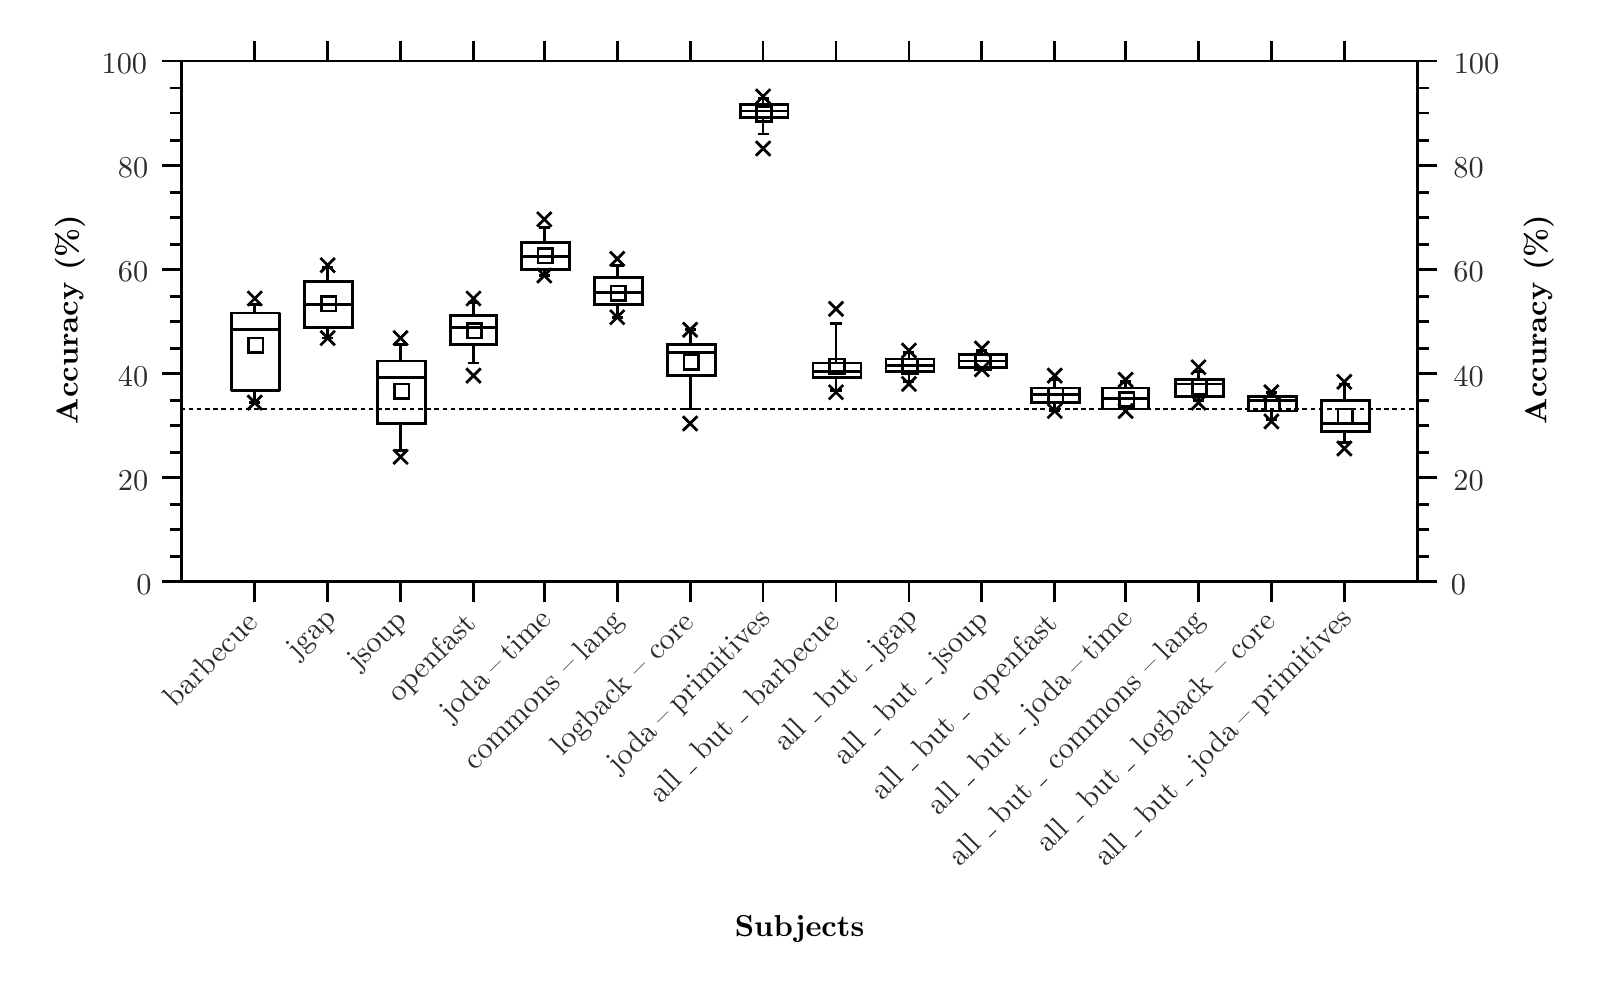
\begin{tikzpicture}{0pt}{0pt}{742pt}{452pt}
	\clip(0pt,452pt) -- (558.587pt,452pt) -- (558.587pt,111.729pt) -- (0pt,111.729pt) -- (0pt,452pt);
\begin{scope}
	\clip(55.7081pt,439.955pt) -- (502.126pt,439.955pt) -- (502.126pt,251.752pt) -- (55.7081pt,251.752pt) -- (55.7081pt,439.955pt);
	\color[rgb]{0,0,0}
	\draw[line width=1pt, line join=bevel, line cap=rect](73.7756pt,348.865pt) -- (91.0903pt,348.865pt) -- (91.0903pt,321.011pt) -- (73.7756pt,321.011pt) -- (73.7756pt,348.865pt);
	\color[rgb]{0,0,0}
	\draw[line width=1pt, line join=bevel, line cap=rect](80.5509pt,316.494pt) -- (83.5622pt,316.494pt);
	\draw[line width=1pt, line join=bevel, line cap=rect](80.5509pt,351.876pt) -- (83.5622pt,351.876pt);
	\draw[line width=1pt, line join=bevel, line cap=rect](82.0566pt,351.876pt) -- (82.0566pt,348.865pt);
	\draw[line width=1pt, line join=bevel, line cap=rect](82.0566pt,316.494pt) -- (82.0566pt,321.011pt);
	\draw[line width=1pt, line join=bevel, line cap=rect](73.7756pt,342.842pt) -- (90.3375pt,342.842pt);
	\draw[line width=1pt, line join=miter, line cap=rect](79.7981pt,318.752pt) -- (84.315pt,314.235pt);
	\draw[line width=1pt, line join=miter, line cap=rect](79.7981pt,314.235pt) -- (84.315pt,318.752pt);
	\draw[line width=1pt, line join=miter, line cap=rect](79.7981pt,356.393pt) -- (84.315pt,351.876pt);
	\draw[line width=1pt, line join=miter, line cap=rect](79.7981pt,351.876pt) -- (84.315pt,356.393pt);
	\draw[line width=1pt, line join=miter, line cap=rect](79.7981pt,339.831pt) -- (85.0678pt,339.831pt) -- (85.0678pt,334.561pt) -- (79.7981pt,334.561pt) -- (79.7981pt,339.831pt);
	\draw[line width=1pt, line join=miter, line cap=rect](100.124pt,360.157pt) -- (117.439pt,360.157pt) -- (117.439pt,343.595pt) -- (100.124pt,343.595pt) -- (100.124pt,360.157pt);
	\draw[line width=1pt, line join=miter, line cap=rect](106.899pt,339.831pt) -- (109.911pt,339.831pt);
	\draw[line width=1pt, line join=miter, line cap=rect](106.899pt,365.427pt) -- (109.911pt,365.427pt);
	\draw[line width=1pt, line join=miter, line cap=rect](108.405pt,365.427pt) -- (108.405pt,360.157pt);
	\draw[line width=1pt, line join=miter, line cap=rect](108.405pt,339.831pt) -- (108.405pt,343.595pt);
	\draw[line width=1pt, line join=miter, line cap=rect](100.124pt,351.876pt) -- (116.686pt,351.876pt);
	\draw[line width=1pt, line join=miter, line cap=rect](106.147pt,342.089pt) -- (110.663pt,337.572pt);
	\draw[line width=1pt, line join=miter, line cap=rect](106.147pt,337.572pt) -- (110.663pt,342.089pt);
	\draw[line width=1pt, line join=miter, line cap=rect](106.147pt,368.438pt) -- (110.663pt,363.921pt);
	\draw[line width=1pt, line join=miter, line cap=rect](106.147pt,363.921pt) -- (110.663pt,368.438pt);
	\draw[line width=1pt, line join=miter, line cap=rect](106.147pt,354.887pt) -- (111.416pt,354.887pt) -- (111.416pt,349.618pt) -- (106.147pt,349.618pt) -- (106.147pt,354.887pt);
	\draw[line width=1pt, line join=miter, line cap=rect](126.472pt,331.55pt) -- (143.787pt,331.55pt) -- (143.787pt,308.966pt) -- (126.472pt,308.966pt) -- (126.472pt,331.55pt);
	\draw[line width=1pt, line join=miter, line cap=rect](133.248pt,299.179pt) -- (136.259pt,299.179pt);
	\draw[line width=1pt, line join=miter, line cap=rect](133.248pt,337.572pt) -- (136.259pt,337.572pt);
	\draw[line width=1pt, line join=miter, line cap=rect](134.753pt,337.572pt) -- (134.753pt,331.55pt);
	\draw[line width=1pt, line join=miter, line cap=rect](134.753pt,299.179pt) -- (134.753pt,308.966pt);
	\draw[line width=1pt, line join=miter, line cap=rect](126.472pt,325.528pt) -- (143.034pt,325.528pt);
	\draw[line width=1pt, line join=miter, line cap=rect](132.495pt,299.179pt) -- (137.012pt,294.662pt);
	\draw[line width=1pt, line join=miter, line cap=rect](132.495pt,294.662pt) -- (137.012pt,299.179pt);
	\draw[line width=1pt, line join=miter, line cap=rect](132.495pt,342.089pt) -- (137.012pt,337.572pt);
	\draw[line width=1pt, line join=miter, line cap=rect](132.495pt,337.572pt) -- (137.012pt,342.089pt);
	\draw[line width=1pt, line join=miter, line cap=rect](132.495pt,323.269pt) -- (137.765pt,323.269pt) -- (137.765pt,317.999pt) -- (132.495pt,317.999pt) -- (132.495pt,323.269pt);
	\draw[line width=1pt, line join=miter, line cap=rect](152.821pt,348.112pt) -- (169.383pt,348.112pt) -- (169.383pt,337.572pt) -- (152.821pt,337.572pt) -- (152.821pt,348.112pt);
	\draw[line width=1pt, line join=miter, line cap=rect](159.596pt,330.797pt) -- (162.607pt,330.797pt);
	\draw[line width=1pt, line join=miter, line cap=rect](159.596pt,352.629pt) -- (162.607pt,352.629pt);
	\draw[line width=1pt, line join=miter, line cap=rect](161.102pt,352.629pt) -- (161.102pt,348.112pt);
	\draw[line width=1pt, line join=miter, line cap=rect](161.102pt,330.797pt) -- (161.102pt,337.572pt);
	\draw[line width=1pt, line join=miter, line cap=rect](152.821pt,343.595pt) -- (169.383pt,343.595pt);
	\draw[line width=1pt, line join=miter, line cap=rect](158.843pt,328.539pt) -- (163.36pt,324.022pt);
	\draw[line width=1pt, line join=miter, line cap=rect](158.843pt,324.022pt) -- (163.36pt,328.539pt);
	\draw[line width=1pt, line join=miter, line cap=rect](158.843pt,356.393pt) -- (163.36pt,351.876pt);
	\draw[line width=1pt, line join=miter, line cap=rect](158.843pt,351.876pt) -- (163.36pt,356.393pt);
	\draw[line width=1pt, line join=miter, line cap=rect](158.843pt,345.101pt) -- (164.113pt,345.101pt) -- (164.113pt,339.831pt) -- (158.843pt,339.831pt) -- (158.843pt,345.101pt);
	\draw[line width=1pt, line join=miter, line cap=rect](178.417pt,374.46pt) -- (195.731pt,374.46pt) -- (195.731pt,364.674pt) -- (178.417pt,364.674pt) -- (178.417pt,374.46pt);
	\draw[line width=1pt, line join=miter, line cap=rect](185.192pt,362.415pt) -- (188.203pt,362.415pt);
	\draw[line width=1pt, line join=miter, line cap=rect](185.192pt,379.73pt) -- (188.203pt,379.73pt);
	\draw[line width=1pt, line join=miter, line cap=rect](186.697pt,379.73pt) -- (186.697pt,374.46pt);
	\draw[line width=1pt, line join=miter, line cap=rect](186.697pt,362.415pt) -- (186.697pt,364.674pt);
	\draw[line width=1pt, line join=miter, line cap=rect](178.417pt,369.191pt) -- (194.978pt,369.191pt);
	\draw[line width=1pt, line join=miter, line cap=rect](184.439pt,364.674pt) -- (188.956pt,360.157pt);
	\draw[line width=1pt, line join=miter, line cap=rect](184.439pt,360.157pt) -- (188.956pt,364.674pt);
	\draw[line width=1pt, line join=miter, line cap=rect](184.439pt,385pt) -- (188.956pt,380.483pt);
	\draw[line width=1pt, line join=miter, line cap=rect](184.439pt,380.483pt) -- (188.956pt,385pt);
	\draw[line width=1pt, line join=miter, line cap=rect](184.439pt,372.202pt) -- (189.709pt,372.202pt) -- (189.709pt,366.932pt) -- (184.439pt,366.932pt) -- (184.439pt,372.202pt);
	\draw[line width=1pt, line join=miter, line cap=rect](204.765pt,361.663pt) -- (222.08pt,361.663pt) -- (222.08pt,351.876pt) -- (204.765pt,351.876pt) -- (204.765pt,361.663pt);
	\draw[line width=1pt, line join=miter, line cap=rect](211.54pt,347.359pt) -- (214.552pt,347.359pt);
	\draw[line width=1pt, line join=miter, line cap=rect](211.54pt,366.179pt) -- (214.552pt,366.179pt);
	\draw[line width=1pt, line join=miter, line cap=rect](213.046pt,366.179pt) -- (213.046pt,361.663pt);
	\draw[line width=1pt, line join=miter, line cap=rect](213.046pt,347.359pt) -- (213.046pt,351.876pt);
	\draw[line width=1pt, line join=miter, line cap=rect](204.765pt,356.393pt) -- (221.327pt,356.393pt);
	\draw[line width=1pt, line join=miter, line cap=rect](210.787pt,349.618pt) -- (215.304pt,345.101pt);
	\draw[line width=1pt, line join=miter, line cap=rect](210.787pt,345.101pt) -- (215.304pt,349.618pt);
	\draw[line width=1pt, line join=miter, line cap=rect](210.787pt,370.696pt) -- (215.304pt,366.179pt);
	\draw[line width=1pt, line join=miter, line cap=rect](210.787pt,366.179pt) -- (215.304pt,370.696pt);
	\draw[line width=1pt, line join=miter, line cap=rect](210.787pt,358.651pt) -- (216.057pt,358.651pt) -- (216.057pt,353.382pt) -- (210.787pt,353.382pt) -- (210.787pt,358.651pt);
	\draw[line width=1pt, line join=miter, line cap=rect](231.113pt,337.572pt) -- (248.428pt,337.572pt) -- (248.428pt,326.28pt) -- (231.113pt,326.28pt) -- (231.113pt,337.572pt);
	\draw[line width=1pt, line join=miter, line cap=rect](237.889pt,314.235pt) -- (240.9pt,314.235pt);
	\draw[line width=1pt, line join=miter, line cap=rect](237.889pt,342.842pt) -- (240.9pt,342.842pt);
	\draw[line width=1pt, line join=miter, line cap=rect](239.394pt,342.842pt) -- (239.394pt,337.572pt);
	\draw[line width=1pt, line join=miter, line cap=rect](239.394pt,314.235pt) -- (239.394pt,326.28pt);
	\draw[line width=1pt, line join=miter, line cap=rect](231.113pt,334.561pt) -- (247.675pt,334.561pt);
	\draw[line width=1pt, line join=miter, line cap=rect](237.136pt,311.224pt) -- (241.653pt,306.707pt);
	\draw[line width=1pt, line join=miter, line cap=rect](237.136pt,306.707pt) -- (241.653pt,311.224pt);
	\draw[line width=1pt, line join=miter, line cap=rect](237.136pt,345.101pt) -- (241.653pt,340.584pt);
	\draw[line width=1pt, line join=miter, line cap=rect](237.136pt,340.584pt) -- (241.653pt,345.101pt);
	\draw[line width=1pt, line join=miter, line cap=rect](237.136pt,333.808pt) -- (242.406pt,333.808pt) -- (242.406pt,328.539pt) -- (237.136pt,328.539pt) -- (237.136pt,333.808pt);
	\draw[line width=1pt, line join=miter, line cap=rect](257.462pt,424.146pt) -- (274.777pt,424.146pt) -- (274.777pt,419.629pt) -- (257.462pt,419.629pt) -- (257.462pt,424.146pt);
	\draw[line width=1pt, line join=miter, line cap=rect](264.237pt,413.607pt) -- (267.248pt,413.607pt);
	\draw[line width=1pt, line join=miter, line cap=rect](264.237pt,426.404pt) -- (267.248pt,426.404pt);
	\draw[line width=1pt, line join=miter, line cap=rect](265.743pt,426.404pt) -- (265.743pt,424.146pt);
	\draw[line width=1pt, line join=miter, line cap=rect](265.743pt,413.607pt) -- (265.743pt,419.629pt);
	\draw[line width=1pt, line join=miter, line cap=rect](257.462pt,421.887pt) -- (274.024pt,421.887pt);
	\draw[line width=1pt, line join=miter, line cap=rect](263.484pt,410.595pt) -- (268.001pt,406.078pt);
	\draw[line width=1pt, line join=miter, line cap=rect](263.484pt,406.078pt) -- (268.001pt,410.595pt);
	\draw[line width=1pt, line join=miter, line cap=rect](263.484pt,429.416pt) -- (268.001pt,424.899pt);
	\draw[line width=1pt, line join=miter, line cap=rect](263.484pt,424.899pt) -- (268.001pt,429.416pt);
	\draw[line width=1pt, line join=miter, line cap=rect](263.484pt,423.393pt) -- (268.754pt,423.393pt) -- (268.754pt,418.123pt) -- (263.484pt,418.123pt) -- (263.484pt,423.393pt);
	\draw[line width=1pt, line join=miter, line cap=rect](283.81pt,330.797pt) -- (301.125pt,330.797pt) -- (301.125pt,325.528pt) -- (283.81pt,325.528pt) -- (283.81pt,330.797pt);
	\draw[line width=1pt, line join=miter, line cap=rect](290.586pt,321.011pt) -- (293.597pt,321.011pt);
	\draw[line width=1pt, line join=miter, line cap=rect](290.586pt,345.101pt) -- (293.597pt,345.101pt);
	\draw[line width=1pt, line join=miter, line cap=rect](292.091pt,345.101pt) -- (292.091pt,330.797pt);
	\draw[line width=1pt, line join=miter, line cap=rect](292.091pt,321.011pt) -- (292.091pt,325.528pt);
	\draw[line width=1pt, line join=miter, line cap=rect](283.81pt,327.786pt) -- (300.372pt,327.786pt);
	\draw[line width=1pt, line join=miter, line cap=rect](289.833pt,322.516pt) -- (294.35pt,317.999pt);
	\draw[line width=1pt, line join=miter, line cap=rect](289.833pt,317.999pt) -- (294.35pt,322.516pt);
	\draw[line width=1pt, line join=miter, line cap=rect](289.833pt,352.629pt) -- (294.35pt,348.112pt);
	\draw[line width=1pt, line join=miter, line cap=rect](289.833pt,348.112pt) -- (294.35pt,352.629pt);
	\draw[line width=1pt, line join=miter, line cap=rect](289.833pt,332.303pt) -- (295.103pt,332.303pt) -- (295.103pt,327.033pt) -- (289.833pt,327.033pt) -- (289.833pt,332.303pt);
	\draw[line width=1pt, line join=miter, line cap=rect](310.159pt,332.303pt) -- (327.473pt,332.303pt) -- (327.473pt,327.786pt) -- (310.159pt,327.786pt) -- (310.159pt,332.303pt);
	\draw[line width=1pt, line join=miter, line cap=rect](316.934pt,324.022pt) -- (319.945pt,324.022pt);
	\draw[line width=1pt, line join=miter, line cap=rect](316.934pt,334.561pt) -- (319.945pt,334.561pt);
	\draw[line width=1pt, line join=miter, line cap=rect](318.44pt,334.561pt) -- (318.44pt,332.303pt);
	\draw[line width=1pt, line join=miter, line cap=rect](318.44pt,324.022pt) -- (318.44pt,327.786pt);
	\draw[line width=1pt, line join=miter, line cap=rect](310.159pt,330.044pt) -- (326.721pt,330.044pt);
	\draw[line width=1pt, line join=miter, line cap=rect](316.181pt,325.528pt) -- (320.698pt,321.011pt);
	\draw[line width=1pt, line join=miter, line cap=rect](316.181pt,321.011pt) -- (320.698pt,325.528pt);
	\draw[line width=1pt, line join=miter, line cap=rect](316.181pt,337.572pt) -- (320.698pt,333.056pt);
	\draw[line width=1pt, line join=miter, line cap=rect](316.181pt,333.056pt) -- (320.698pt,337.572pt);
	\draw[line width=1pt, line join=miter, line cap=rect](316.181pt,332.303pt) -- (321.451pt,332.303pt) -- (321.451pt,327.033pt) -- (316.181pt,327.033pt) -- (316.181pt,332.303pt);
	\draw[line width=1pt, line join=miter, line cap=rect](336.507pt,333.808pt) -- (353.822pt,333.808pt) -- (353.822pt,329.292pt) -- (336.507pt,329.292pt) -- (336.507pt,333.808pt);
	\draw[line width=1pt, line join=miter, line cap=rect](343.282pt,328.539pt) -- (346.294pt,328.539pt);
	\draw[line width=1pt, line join=miter, line cap=rect](343.282pt,335.314pt) -- (346.294pt,335.314pt);
	\draw[line width=1pt, line join=miter, line cap=rect](344.788pt,335.314pt) -- (344.788pt,333.808pt);
	\draw[line width=1pt, line join=miter, line cap=rect](344.788pt,328.539pt) -- (344.788pt,329.292pt);
	\draw[line width=1pt, line join=miter, line cap=rect](336.507pt,331.55pt) -- (353.069pt,331.55pt);
	\draw[line width=1pt, line join=miter, line cap=rect](342.53pt,330.797pt) -- (347.047pt,326.28pt);
	\draw[line width=1pt, line join=miter, line cap=rect](342.53pt,326.28pt) -- (347.047pt,330.797pt);
	\draw[line width=1pt, line join=miter, line cap=rect](342.53pt,338.325pt) -- (347.047pt,333.808pt);
	\draw[line width=1pt, line join=miter, line cap=rect](342.53pt,333.808pt) -- (347.047pt,338.325pt);
	\draw[line width=1pt, line join=miter, line cap=rect](342.53pt,333.808pt) -- (347.799pt,333.808pt) -- (347.799pt,328.539pt) -- (342.53pt,328.539pt) -- (342.53pt,333.808pt);
	\draw[line width=1pt, line join=miter, line cap=rect](362.856pt,321.763pt) -- (380.17pt,321.763pt) -- (380.17pt,316.494pt) -- (362.856pt,316.494pt) -- (362.856pt,321.763pt);
	\draw[line width=1pt, line join=miter, line cap=rect](369.631pt,313.482pt) -- (372.642pt,313.482pt);
	\draw[line width=1pt, line join=miter, line cap=rect](369.631pt,324.775pt) -- (372.642pt,324.775pt);
	\draw[line width=1pt, line join=miter, line cap=rect](371.137pt,324.775pt) -- (371.137pt,321.763pt);
	\draw[line width=1pt, line join=miter, line cap=rect](371.137pt,313.482pt) -- (371.137pt,316.494pt);
	\draw[line width=1pt, line join=miter, line cap=rect](362.856pt,319.505pt) -- (379.418pt,319.505pt);
	\draw[line width=1pt, line join=miter, line cap=rect](368.878pt,315.741pt) -- (373.395pt,311.224pt);
	\draw[line width=1pt, line join=miter, line cap=rect](368.878pt,311.224pt) -- (373.395pt,315.741pt);
	\draw[line width=1pt, line join=miter, line cap=rect](368.878pt,328.539pt) -- (373.395pt,324.022pt);
	\draw[line width=1pt, line join=miter, line cap=rect](368.878pt,324.022pt) -- (373.395pt,328.539pt);
	\draw[line width=1pt, line join=miter, line cap=rect](368.878pt,321.763pt) -- (374.148pt,321.763pt) -- (374.148pt,316.494pt) -- (368.878pt,316.494pt) -- (368.878pt,321.763pt);
	\draw[line width=1pt, line join=miter, line cap=rect](388.451pt,321.763pt) -- (405.013pt,321.763pt) -- (405.013pt,314.235pt) -- (388.451pt,314.235pt) -- (388.451pt,321.763pt);
	\draw[line width=1pt, line join=miter, line cap=rect](395.227pt,314.235pt) -- (398.238pt,314.235pt);
	\draw[line width=1pt, line join=miter, line cap=rect](395.227pt,324.022pt) -- (398.238pt,324.022pt);
	\draw[line width=1pt, line join=miter, line cap=rect](396.732pt,324.022pt) -- (396.732pt,321.763pt);

	\draw[line width=1pt, line join=miter, line cap=rect](388.451pt,317.999pt) -- (405.013pt,317.999pt);
	\draw[line width=1pt, line join=miter, line cap=rect](394.474pt,315.741pt) -- (398.991pt,311.224pt);
	\draw[line width=1pt, line join=miter, line cap=rect](394.474pt,311.224pt) -- (398.991pt,315.741pt);
	\draw[line width=1pt, line join=miter, line cap=rect](394.474pt,327.033pt) -- (398.991pt,322.516pt);
	\draw[line width=1pt, line join=miter, line cap=rect](394.474pt,322.516pt) -- (398.991pt,327.033pt);
	\draw[line width=1pt, line join=miter, line cap=rect](394.474pt,320.258pt) -- (399.743pt,320.258pt) -- (399.743pt,314.988pt) -- (394.474pt,314.988pt) -- (394.474pt,320.258pt);
	\draw[line width=1pt, line join=miter, line cap=rect](414.8pt,324.775pt) -- (432.114pt,324.775pt) -- (432.114pt,318.752pt) -- (414.8pt,318.752pt) -- (414.8pt,324.775pt);
	\draw[line width=1pt, line join=miter, line cap=rect](421.575pt,317.247pt) -- (424.586pt,317.247pt);
	\draw[line width=1pt, line join=miter, line cap=rect](421.575pt,327.786pt) -- (424.586pt,327.786pt);
	\draw[line width=1pt, line join=miter, line cap=rect](423.081pt,327.786pt) -- (423.081pt,324.775pt);
	\draw[line width=1pt, line join=miter, line cap=rect](423.081pt,317.247pt) -- (423.081pt,318.752pt);
	\draw[line width=1pt, line join=miter, line cap=rect](414.8pt,323.269pt) -- (431.362pt,323.269pt);
	\draw[line width=1pt, line join=miter, line cap=rect](420.822pt,318.752pt) -- (425.339pt,314.235pt);
	\draw[line width=1pt, line join=miter, line cap=rect](420.822pt,314.235pt) -- (425.339pt,318.752pt);
	\draw[line width=1pt, line join=miter, line cap=rect](420.822pt,331.55pt) -- (425.339pt,327.033pt);
	\draw[line width=1pt, line join=miter, line cap=rect](420.822pt,327.033pt) -- (425.339pt,331.55pt);
	\draw[line width=1pt, line join=miter, line cap=rect](420.822pt,324.775pt) -- (426.092pt,324.775pt) -- (426.092pt,319.505pt) -- (420.822pt,319.505pt) -- (420.822pt,324.775pt);
	\draw[line width=1pt, line join=miter, line cap=rect](441.148pt,318.752pt) -- (458.463pt,318.752pt) -- (458.463pt,313.482pt) -- (441.148pt,313.482pt) -- (441.148pt,318.752pt);
	\draw[line width=1pt, line join=miter, line cap=rect](447.923pt,310.471pt) -- (450.935pt,310.471pt);
	\draw[line width=1pt, line join=miter, line cap=rect](447.923pt,320.258pt) -- (450.935pt,320.258pt);
	\draw[line width=1pt, line join=miter, line cap=rect](449.429pt,320.258pt) -- (449.429pt,318.752pt);
	\draw[line width=1pt, line join=miter, line cap=rect](449.429pt,310.471pt) -- (449.429pt,313.482pt);
	\draw[line width=1pt, line join=miter, line cap=rect](441.148pt,317.247pt) -- (457.71pt,317.247pt);
	\draw[line width=1pt, line join=miter, line cap=rect](447.171pt,311.977pt) -- (451.688pt,307.46pt);
	\draw[line width=1pt, line join=miter, line cap=rect](447.171pt,307.46pt) -- (451.688pt,311.977pt);
	\draw[line width=1pt, line join=miter, line cap=rect](447.171pt,322.516pt) -- (451.688pt,317.999pt);
	\draw[line width=1pt, line join=miter, line cap=rect](447.171pt,317.999pt) -- (451.688pt,322.516pt);
	\draw[line width=1pt, line join=miter, line cap=rect](447.171pt,318.752pt) -- (452.44pt,318.752pt) -- (452.44pt,313.482pt) -- (447.171pt,313.482pt) -- (447.171pt,318.752pt);
	\draw[line width=1pt, line join=miter, line cap=rect](467.497pt,317.247pt) -- (484.811pt,317.247pt) -- (484.811pt,305.954pt) -- (467.497pt,305.954pt) -- (467.497pt,317.247pt);
	\draw[line width=1pt, line join=miter, line cap=rect](474.272pt,302.19pt) -- (477.283pt,302.19pt);
	\draw[line width=1pt, line join=miter, line cap=rect](474.272pt,323.269pt) -- (477.283pt,323.269pt);
	\draw[line width=1pt, line join=miter, line cap=rect](475.777pt,323.269pt) -- (475.777pt,317.247pt);
	\draw[line width=1pt, line join=miter, line cap=rect](475.777pt,302.19pt) -- (475.777pt,305.954pt);
	\draw[line width=1pt, line join=miter, line cap=rect](467.497pt,308.966pt) -- (484.058pt,308.966pt);
	\draw[line width=1pt, line join=miter, line cap=rect](473.519pt,302.19pt) -- (478.036pt,297.673pt);
	\draw[line width=1pt, line join=miter, line cap=rect](473.519pt,297.673pt) -- (478.036pt,302.19pt);
	\draw[line width=1pt, line join=miter, line cap=rect](473.519pt,326.28pt) -- (478.036pt,321.763pt);
	\draw[line width=1pt, line join=miter, line cap=rect](473.519pt,321.763pt) -- (478.036pt,326.28pt);
	\draw[line width=1pt, line join=miter, line cap=rect](473.519pt,314.235pt) -- (478.789pt,314.235pt) -- (478.789pt,308.966pt) -- (473.519pt,308.966pt) -- (473.519pt,314.235pt);


	\draw[line width=1pt, dash pattern=on 0.024cm off 0.08cm, dash phase=0pt, line join=miter, line cap=rect](55.7081pt,314.235pt) -- (528.474pt,314.235pt);
\end{scope}
\begin{scope}
	\color[rgb]{0,0,0}
	\pgftext[center, base, at={\pgfpoint{18.0675pt}{346.606pt}},rotate=90]{\fontsize{11}{0}\selectfont{\textbf{Accuracy (\%)}}}
	\color[rgb]{0.172549,0.172549,0.172549}
	\pgftext[center, base, at={\pgfpoint{42.0163pt}{247.235pt}}]{\fontsize{11}{0}\selectfont{0}}
	\pgftext[center, base, at={\pgfpoint{38.1111pt}{284.876pt}}]{\fontsize{11}{0}\selectfont{20}}
	\pgftext[center, base, at={\pgfpoint{38.1111pt}{322.516pt}}]{\fontsize{11}{0}\selectfont{40}}
	\pgftext[center, base, at={\pgfpoint{38.1111pt}{360.157pt}}]{\fontsize{11}{0}\selectfont{60}}
	\pgftext[center, base, at={\pgfpoint{38.1111pt}{397.798pt}}]{\fontsize{11}{0}\selectfont{80}}
	\pgftext[center, base, at={\pgfpoint{34.9587pt}{435.438pt}}]{\fontsize{11}{0}\selectfont{100}}
	\color[rgb]{0,0,0}
	\draw[line width=1pt, line join=bevel, line cap=rect](55.7081pt,260.786pt) -- (51.9441pt,260.786pt);
	\draw[line width=1pt, line join=bevel, line cap=rect](55.7081pt,279.606pt) -- (51.9441pt,279.606pt);
	\draw[line width=1pt, line join=bevel, line cap=rect](55.7081pt,298.426pt) -- (51.9441pt,298.426pt);
	\draw[line width=1pt, line join=bevel, line cap=rect](55.7081pt,317.247pt) -- (51.9441pt,317.247pt);
	\draw[line width=1pt, line join=bevel, line cap=rect](55.7081pt,336.067pt) -- (51.9441pt,336.067pt);
	\draw[line width=1pt, line join=bevel, line cap=rect](55.7081pt,354.887pt) -- (51.9441pt,354.887pt);
	\draw[line width=1pt, line join=bevel, line cap=rect](55.7081pt,373.707pt) -- (51.9441pt,373.707pt);
	\draw[line width=1pt, line join=bevel, line cap=rect](55.7081pt,392.528pt) -- (51.9441pt,392.528pt);
	\draw[line width=1pt, line join=bevel, line cap=rect](55.7081pt,411.348pt) -- (51.9441pt,411.348pt);
	\draw[line width=1pt, line join=bevel, line cap=rect](55.7081pt,430.168pt) -- (51.9441pt,430.168pt);
	\draw[line width=1pt, line join=bevel, line cap=rect](55.7081pt,270.572pt) -- (51.9441pt,270.572pt);
	\draw[line width=1pt, line join=bevel, line cap=rect](55.7081pt,308.213pt) -- (51.9441pt,308.213pt);
	\draw[line width=1pt, line join=bevel, line cap=rect](55.7081pt,345.853pt) -- (51.9441pt,345.853pt);
	\draw[line width=1pt, line join=bevel, line cap=rect](55.7081pt,383.494pt) -- (51.9441pt,383.494pt);
	\draw[line width=1pt, line join=bevel, line cap=rect](55.7081pt,421.135pt) -- (51.9441pt,421.135pt);
	\draw[line width=1pt, line join=bevel, line cap=rect](55.7081pt,251.752pt) -- (48.9328pt,251.752pt);
	\draw[line width=1pt, line join=bevel, line cap=rect](55.7081pt,289.393pt) -- (48.9328pt,289.393pt);
	\draw[line width=1pt, line join=bevel, line cap=rect](55.7081pt,327.033pt) -- (48.9328pt,327.033pt);
	\draw[line width=1pt, line join=bevel, line cap=rect](55.7081pt,364.674pt) -- (48.9328pt,364.674pt);
	\draw[line width=1pt, line join=bevel, line cap=rect](55.7081pt,402.314pt) -- (48.9328pt,402.314pt);
	\draw[line width=1pt, line join=bevel, line cap=rect](55.7081pt,439.955pt) -- (48.9328pt,439.955pt);
	\draw[line width=1pt, line join=bevel, line cap=rect](55.7081pt,439.955pt) -- (55.7081pt,251.752pt);
	\pgftext[center, base, at={\pgfpoint{548.8pt}{346.606pt}},rotate=90]{\fontsize{11}{0}\selectfont{\textbf{Accuracy (\%)}}}
	\color[rgb]{0.172549,0.172549,0.172549}
	\pgftext[center, base, at={\pgfpoint{517.041pt}{247.235pt}}]{\fontsize{11}{0}\selectfont{0}}
	\pgftext[center, base, at={\pgfpoint{520.664pt}{284.876pt}}]{\fontsize{11}{0}\selectfont{20}}
	\pgftext[center, base, at={\pgfpoint{520.664pt}{322.516pt}}]{\fontsize{11}{0}\selectfont{40}}
	\pgftext[center, base, at={\pgfpoint{520.664pt}{360.157pt}}]{\fontsize{11}{0}\selectfont{60}}
	\pgftext[center, base, at={\pgfpoint{520.664pt}{397.798pt}}]{\fontsize{11}{0}\selectfont{80}}
	\pgftext[center, base, at={\pgfpoint{523.534pt}{435.438pt}}]{\fontsize{11}{0}\selectfont{100}}
	\color[rgb]{0,0,0}
	\draw[line width=1pt, line join=bevel, line cap=rect](502.126pt,260.786pt) -- (505.89pt,260.786pt);
	\draw[line width=1pt, line join=bevel, line cap=rect](502.126pt,279.606pt) -- (505.89pt,279.606pt);
	\draw[line width=1pt, line join=bevel, line cap=rect](502.126pt,298.426pt) -- (505.89pt,298.426pt);
	\draw[line width=1pt, line join=bevel, line cap=rect](502.126pt,317.247pt) -- (505.89pt,317.247pt);
	\draw[line width=1pt, line join=bevel, line cap=rect](502.126pt,336.067pt) -- (505.89pt,336.067pt);
	\draw[line width=1pt, line join=bevel, line cap=rect](502.126pt,354.887pt) -- (505.89pt,354.887pt);
	\draw[line width=1pt, line join=bevel, line cap=rect](502.126pt,373.707pt) -- (505.89pt,373.707pt);
	\draw[line width=1pt, line join=bevel, line cap=rect](502.126pt,392.528pt) -- (505.89pt,392.528pt);
	\draw[line width=1pt, line join=bevel, line cap=rect](502.126pt,411.348pt) -- (505.89pt,411.348pt);
	\draw[line width=1pt, line join=bevel, line cap=rect](502.126pt,430.168pt) -- (505.89pt,430.168pt);
	\draw[line width=1pt, line join=bevel, line cap=rect](502.126pt,270.572pt) -- (505.89pt,270.572pt);
	\draw[line width=1pt, line join=bevel, line cap=rect](502.126pt,308.213pt) -- (505.89pt,308.213pt);
	\draw[line width=1pt, line join=bevel, line cap=rect](502.126pt,345.853pt) -- (505.89pt,345.853pt);
	\draw[line width=1pt, line join=bevel, line cap=rect](502.126pt,383.494pt) -- (505.89pt,383.494pt);
	\draw[line width=1pt, line join=bevel, line cap=rect](502.126pt,421.135pt) -- (505.89pt,421.135pt);
	\draw[line width=1pt, line join=bevel, line cap=rect](502.126pt,251.752pt) -- (508.901pt,251.752pt);
	\draw[line width=1pt, line join=bevel, line cap=rect](502.126pt,289.393pt) -- (508.901pt,289.393pt);
	\draw[line width=1pt, line join=bevel, line cap=rect](502.126pt,327.033pt) -- (508.901pt,327.033pt);
	\draw[line width=1pt, line join=bevel, line cap=rect](502.126pt,364.674pt) -- (508.901pt,364.674pt);
	\draw[line width=1pt, line join=bevel, line cap=rect](502.126pt,402.314pt) -- (508.901pt,402.314pt);
	\draw[line width=1pt, line join=bevel, line cap=rect](502.126pt,439.955pt) -- (508.901pt,439.955pt);
	\draw[line width=1pt, line join=bevel, line cap=rect](502.126pt,439.955pt) -- (502.126pt,251.752pt);
	\pgftext[center, base, at={\pgfpoint{278.917pt}{123.774pt}}]{\fontsize{11}{0}\selectfont{\textbf{Subjects}}}
	\color[rgb]{0.172549,0.172549,0.172549}
	\pgftext[center, base, at={\pgfpoint{68.4991pt}{221.267pt}},rotate=45]{\fontsize{11}{0}\selectfont{barbecue}}
	\pgftext[center, base, at={\pgfpoint{104.654pt}{231.073pt}},rotate=45]{\fontsize{11}{0}\selectfont{jgap}}
	\pgftext[center, base, at={\pgfpoint{128.445pt}{228.516pt}},rotate=45]{\fontsize{11}{0}\selectfont{jsoup}}
	\pgftext[center, base, at={\pgfpoint{148.222pt}{221.945pt}},rotate=45]{\fontsize{11}{0}\selectfont{openfast}}
	\pgftext[center, base, at={\pgfpoint{160.198pt}{208.325pt}},rotate=45]{\fontsize{11}{0}\selectfont{joda}}
	\pgftext[center, base, at={\pgfpoint{171.111pt}{219.238pt}},rotate=45]{\fontsize{11}{0}\selectfont{--}}
	\pgftext[center, base, at={\pgfpoint{182.11pt}{230.238pt}},rotate=45]{\fontsize{11}{0}\selectfont{time}}
	\pgftext[center, base, at={\pgfpoint{177.272pt}{199.051pt}},rotate=45]{\fontsize{11}{0}\selectfont{commons}}
	\pgftext[center, base, at={\pgfpoint{197.542pt}{219.321pt}},rotate=45]{\fontsize{11}{0}\selectfont{--}}
	\pgftext[center, base, at={\pgfpoint{208.405pt}{230.184pt}},rotate=45]{\fontsize{11}{0}\selectfont{lang}}
	\pgftext[center, base, at={\pgfpoint{205.896pt}{201.326pt}},rotate=45]{\fontsize{11}{0}\selectfont{logback}}
	\pgftext[center, base, at={\pgfpoint{223.117pt}{218.547pt}},rotate=45]{\fontsize{11}{0}\selectfont{--}}
	\pgftext[center, base, at={\pgfpoint{234.342pt}{229.772pt}},rotate=45]{\fontsize{11}{0}\selectfont{core}}
	\pgftext[center, base, at={\pgfpoint{220.612pt}{189.694pt}},rotate=45]{\fontsize{11}{0}\selectfont{joda}}
	\pgftext[center, base, at={\pgfpoint{231.525pt}{200.607pt}},rotate=45]{\fontsize{11}{0}\selectfont{--}}
	\pgftext[center, base, at={\pgfpoint{252.027pt}{221.109pt}},rotate=45]{\fontsize{11}{0}\selectfont{primitives}}
	\pgftext[center, base, at={\pgfpoint{232.684pt}{175.417pt}},rotate=45]{\fontsize{11}{0}\selectfont{all}}
	\pgftext[center, base, at={\pgfpoint{240.498pt}{183.231pt}},rotate=45]{\fontsize{11}{0}\selectfont{\_}}
	\pgftext[center, base, at={\pgfpoint{249.743pt}{192.476pt}},rotate=45]{\fontsize{11}{0}\selectfont{but}}
	\pgftext[center, base, at={\pgfpoint{258.988pt}{201.721pt}},rotate=45]{\fontsize{11}{0}\selectfont{\_}}
	\pgftext[center, base, at={\pgfpoint{278.584pt}{221.317pt}},rotate=45]{\fontsize{11}{0}\selectfont{barbecue}}
	\pgftext[center, base, at={\pgfpoint{277.663pt}{194.048pt}},rotate=45]{\fontsize{11}{0}\selectfont{all}}
	\pgftext[center, base, at={\pgfpoint{285.478pt}{201.862pt}},rotate=45]{\fontsize{11}{0}\selectfont{\_}}
	\pgftext[center, base, at={\pgfpoint{294.722pt}{211.107pt}},rotate=45]{\fontsize{11}{0}\selectfont{but}}
	\pgftext[center, base, at={\pgfpoint{303.967pt}{220.352pt}},rotate=45]{\fontsize{11}{0}\selectfont{\_}}
	\pgftext[center, base, at={\pgfpoint{314.738pt}{231.123pt}},rotate=45]{\fontsize{11}{0}\selectfont{jgap}}
	\pgftext[center, base, at={\pgfpoint{299.221pt}{189.257pt}},rotate=45]{\fontsize{11}{0}\selectfont{all}}
	\pgftext[center, base, at={\pgfpoint{307.035pt}{197.072pt}},rotate=45]{\fontsize{11}{0}\selectfont{\_}}
	\pgftext[center, base, at={\pgfpoint{316.28pt}{206.317pt}},rotate=45]{\fontsize{11}{0}\selectfont{but}}
	\pgftext[center, base, at={\pgfpoint{325.525pt}{215.561pt}},rotate=45]{\fontsize{11}{0}\selectfont{\_}}
	\pgftext[center, base, at={\pgfpoint{338.529pt}{228.566pt}},rotate=45]{\fontsize{11}{0}\selectfont{jsoup}}
	\pgftext[center, base, at={\pgfpoint{312.794pt}{176.482pt}},rotate=45]{\fontsize{11}{0}\selectfont{all}}
	\pgftext[center, base, at={\pgfpoint{320.608pt}{184.296pt}},rotate=45]{\fontsize{11}{0}\selectfont{\_}}
	\pgftext[center, base, at={\pgfpoint{329.853pt}{193.541pt}},rotate=45]{\fontsize{11}{0}\selectfont{but}}
	\pgftext[center, base, at={\pgfpoint{339.098pt}{202.786pt}},rotate=45]{\fontsize{11}{0}\selectfont{\_}}
	\pgftext[center, base, at={\pgfpoint{358.307pt}{221.995pt}},rotate=45]{\fontsize{11}{0}\selectfont{openfast}}
	\pgftext[center, base, at={\pgfpoint{333.066pt}{171.159pt}},rotate=45]{\fontsize{11}{0}\selectfont{all}}
	\pgftext[center, base, at={\pgfpoint{340.88pt}{178.973pt}},rotate=45]{\fontsize{11}{0}\selectfont{\_}}
	\pgftext[center, base, at={\pgfpoint{350.125pt}{188.218pt}},rotate=45]{\fontsize{11}{0}\selectfont{but}}
	\pgftext[center, base, at={\pgfpoint{359.37pt}{197.463pt}},rotate=45]{\fontsize{11}{0}\selectfont{\_}}
	\pgftext[center, base, at={\pgfpoint{370.283pt}{208.375pt}},rotate=45]{\fontsize{11}{0}\selectfont{joda}}
	\pgftext[center, base, at={\pgfpoint{381.195pt}{219.288pt}},rotate=45]{\fontsize{11}{0}\selectfont{--}}
	\pgftext[center, base, at={\pgfpoint{392.195pt}{230.287pt}},rotate=45]{\fontsize{11}{0}\selectfont{time}}
	\pgftext[center, base, at={\pgfpoint{340.783pt}{152.527pt}},rotate=45]{\fontsize{11}{0}\selectfont{all}}
	\pgftext[center, base, at={\pgfpoint{348.598pt}{160.342pt}},rotate=45]{\fontsize{11}{0}\selectfont{\_}}
	\pgftext[center, base, at={\pgfpoint{357.842pt}{169.587pt}},rotate=45]{\fontsize{11}{0}\selectfont{but}}
	\pgftext[center, base, at={\pgfpoint{367.087pt}{178.831pt}},rotate=45]{\fontsize{11}{0}\selectfont{\_}}
	\pgftext[center, base, at={\pgfpoint{387.357pt}{199.101pt}},rotate=45]{\fontsize{11}{0}\selectfont{commons}}
	\pgftext[center, base, at={\pgfpoint{407.627pt}{219.371pt}},rotate=45]{\fontsize{11}{0}\selectfont{--}}
	\pgftext[center, base, at={\pgfpoint{418.489pt}{230.233pt}},rotate=45]{\fontsize{11}{0}\selectfont{lang}}
	\pgftext[center, base, at={\pgfpoint{372.455pt}{157.851pt}},rotate=45]{\fontsize{11}{0}\selectfont{all}}
	\pgftext[center, base, at={\pgfpoint{380.269pt}{165.665pt}},rotate=45]{\fontsize{11}{0}\selectfont{\_}}
	\pgftext[center, base, at={\pgfpoint{389.514pt}{174.91pt}},rotate=45]{\fontsize{11}{0}\selectfont{but}}
	\pgftext[center, base, at={\pgfpoint{398.759pt}{184.155pt}},rotate=45]{\fontsize{11}{0}\selectfont{\_}}
	\pgftext[center, base, at={\pgfpoint{415.98pt}{201.376pt}},rotate=45]{\fontsize{11}{0}\selectfont{logback}}
	\pgftext[center, base, at={\pgfpoint{433.202pt}{218.597pt}},rotate=45]{\fontsize{11}{0}\selectfont{--}}
	\pgftext[center, base, at={\pgfpoint{444.426pt}{229.822pt}},rotate=45]{\fontsize{11}{0}\selectfont{core}}
	\pgftext[center, base, at={\pgfpoint{393.48pt}{152.527pt}},rotate=45]{\fontsize{11}{0}\selectfont{all}}
	\pgftext[center, base, at={\pgfpoint{401.294pt}{160.342pt}},rotate=45]{\fontsize{11}{0}\selectfont{\_}}
	\pgftext[center, base, at={\pgfpoint{410.539pt}{169.587pt}},rotate=45]{\fontsize{11}{0}\selectfont{but}}
	\pgftext[center, base, at={\pgfpoint{419.784pt}{178.831pt}},rotate=45]{\fontsize{11}{0}\selectfont{\_}}
	\pgftext[center, base, at={\pgfpoint{430.697pt}{189.744pt}},rotate=45]{\fontsize{11}{0}\selectfont{joda}}
	\pgftext[center, base, at={\pgfpoint{441.609pt}{200.656pt}},rotate=45]{\fontsize{11}{0}\selectfont{--}}
	\pgftext[center, base, at={\pgfpoint{462.112pt}{221.159pt}},rotate=45]{\fontsize{11}{0}\selectfont{primitives}}
	\color[rgb]{0,0,0}
	\draw[line width=1pt, line join=bevel, line cap=rect](82.0566pt,251.752pt) -- (82.0566pt,244.977pt);
	\draw[line width=1pt, line join=bevel, line cap=rect](108.405pt,251.752pt) -- (108.405pt,244.977pt);
	\draw[line width=1pt, line join=bevel, line cap=rect](134.753pt,251.752pt) -- (134.753pt,244.977pt);
	\draw[line width=1pt, line join=bevel, line cap=rect](161.102pt,251.752pt) -- (161.102pt,244.977pt);
	\draw[line width=1pt, line join=bevel, line cap=rect](186.697pt,251.752pt) -- (186.697pt,244.977pt);
	\draw[line width=1pt, line join=bevel, line cap=rect](213.046pt,251.752pt) -- (213.046pt,244.977pt);
	\draw[line width=1pt, line join=bevel, line cap=rect](239.394pt,251.752pt) -- (239.394pt,244.977pt);
	\draw[line width=1pt, line join=bevel, line cap=rect](265.743pt,251.752pt) -- (265.743pt,244.977pt);
	\draw[line width=1pt, line join=bevel, line cap=rect](292.091pt,251.752pt) -- (292.091pt,244.977pt);
	\draw[line width=1pt, line join=bevel, line cap=rect](318.44pt,251.752pt) -- (318.44pt,244.977pt);
	\draw[line width=1pt, line join=bevel, line cap=rect](344.788pt,251.752pt) -- (344.788pt,244.977pt);
	\draw[line width=1pt, line join=bevel, line cap=rect](371.137pt,251.752pt) -- (371.137pt,244.977pt);
	\draw[line width=1pt, line join=bevel, line cap=rect](396.732pt,251.752pt) -- (396.732pt,244.977pt);
	\draw[line width=1pt, line join=bevel, line cap=rect](423.081pt,251.752pt) -- (423.081pt,244.977pt);
	\draw[line width=1pt, line join=bevel, line cap=rect](449.429pt,251.752pt) -- (449.429pt,244.977pt);
	\draw[line width=1pt, line join=bevel, line cap=rect](475.777pt,251.752pt) -- (475.777pt,244.977pt);
	\draw[line width=1pt, line join=bevel, line cap=rect](55.7081pt,251.752pt) -- (502.126pt,251.752pt);
	\draw[line width=1pt, line join=bevel, line cap=rect](82.0566pt,439.955pt) -- (82.0566pt,446.73pt);
	\draw[line width=1pt, line join=bevel, line cap=rect](108.405pt,439.955pt) -- (108.405pt,446.73pt);
	\draw[line width=1pt, line join=bevel, line cap=rect](134.753pt,439.955pt) -- (134.753pt,446.73pt);
	\draw[line width=1pt, line join=bevel, line cap=rect](161.102pt,439.955pt) -- (161.102pt,446.73pt);
	\draw[line width=1pt, line join=bevel, line cap=rect](186.697pt,439.955pt) -- (186.697pt,446.73pt);
	\draw[line width=1pt, line join=bevel, line cap=rect](213.046pt,439.955pt) -- (213.046pt,446.73pt);
	\draw[line width=1pt, line join=bevel, line cap=rect](239.394pt,439.955pt) -- (239.394pt,446.73pt);
	\draw[line width=1pt, line join=bevel, line cap=rect](265.743pt,439.955pt) -- (265.743pt,446.73pt);
	\draw[line width=1pt, line join=bevel, line cap=rect](292.091pt,439.955pt) -- (292.091pt,446.73pt);
	\draw[line width=1pt, line join=bevel, line cap=rect](318.44pt,439.955pt) -- (318.44pt,446.73pt);
	\draw[line width=1pt, line join=bevel, line cap=rect](344.788pt,439.955pt) -- (344.788pt,446.73pt);
	\draw[line width=1pt, line join=bevel, line cap=rect](371.137pt,439.955pt) -- (371.137pt,446.73pt);
	\draw[line width=1pt, line join=bevel, line cap=rect](396.732pt,439.955pt) -- (396.732pt,446.73pt);
	\draw[line width=1pt, line join=bevel, line cap=rect](423.081pt,439.955pt) -- (423.081pt,446.73pt);
	\draw[line width=1pt, line join=bevel, line cap=rect](449.429pt,439.955pt) -- (449.429pt,446.73pt);
	\draw[line width=1pt, line join=bevel, line cap=rect](475.777pt,439.955pt) -- (475.777pt,446.73pt);
	\draw[line width=1pt, line join=bevel, line cap=rect](55.7081pt,439.955pt) -- (502.126pt,439.955pt);
\end{scope}
\end{tikzpicture}

    \end{adjustbox}
    \caption{Method-level training and prediction accuracy over the eight test subjects and sets of \textit{all\_but\_subject} subjects.}
    \label{fig:prediction_method_graph}
  \end{figure}
}

\subsection{Optimization and Generalization}
\frame{\frametitle{Optimization and Generalization}
\begin{figure}[!tb]
  \centering
  \begin{adjustbox}{max size={.95\textwidth}{.95\textheight}}
    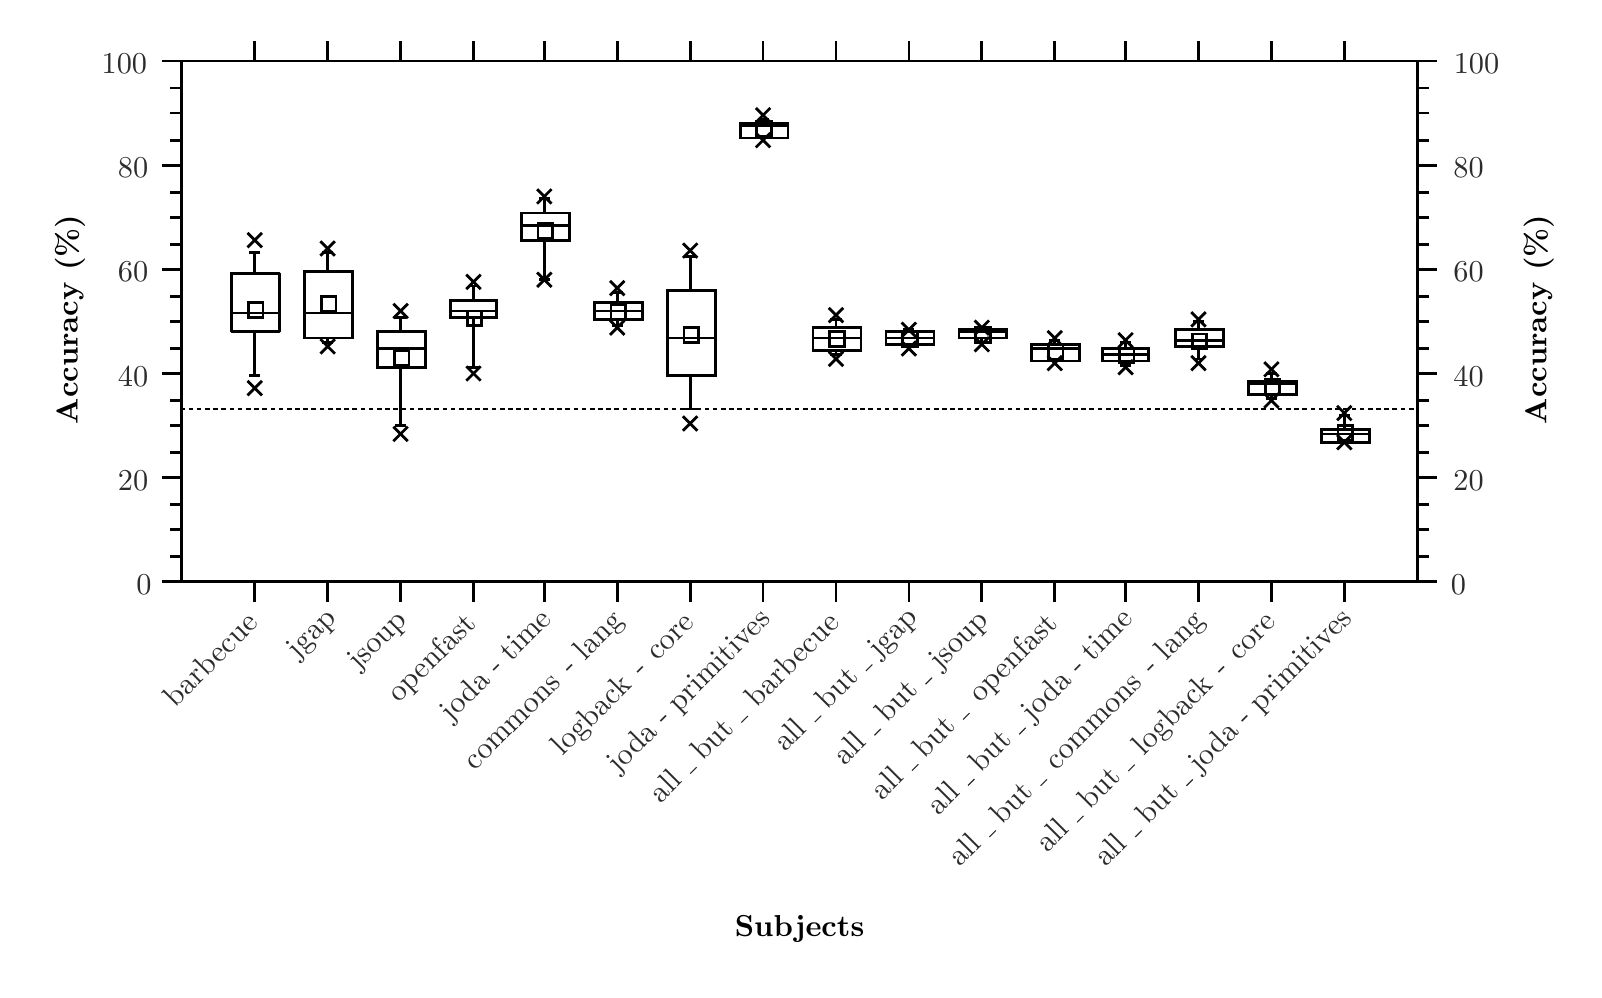
\begin{tikzpicture}{0pt}{0pt}{742pt}{452pt}
	\clip(0pt,452pt) -- (558.587pt,452pt) -- (558.587pt,111.729pt) -- (0pt,111.729pt) -- (0pt,452pt);
\begin{scope}
	\clip(55.7081pt,439.955pt) -- (502.126pt,439.955pt) -- (502.126pt,251.752pt) -- (55.7081pt,251.752pt) -- (55.7081pt,439.955pt);
	\color[rgb]{0,0,0}
	\draw[line width=1pt, line join=bevel, line cap=rect](73.7756pt,363.168pt) -- (91.0903pt,363.168pt) -- (91.0903pt,342.089pt) -- (73.7756pt,342.089pt) -- (73.7756pt,363.168pt);
	\color[rgb]{0,0,0}
	\draw[line width=1pt, line join=bevel, line cap=rect](80.5509pt,326.28pt) -- (83.5622pt,326.28pt);
	\draw[line width=1pt, line join=bevel, line cap=rect](80.5509pt,370.696pt) -- (83.5622pt,370.696pt);
	\draw[line width=1pt, line join=bevel, line cap=rect](82.0566pt,370.696pt) -- (82.0566pt,363.168pt);
	\draw[line width=1pt, line join=bevel, line cap=rect](82.0566pt,326.28pt) -- (82.0566pt,342.089pt);
	\draw[line width=1pt, line join=bevel, line cap=rect](73.7756pt,348.865pt) -- (90.3375pt,348.865pt);
	\draw[line width=1pt, line join=miter, line cap=rect](79.7981pt,324.022pt) -- (84.315pt,319.505pt);
	\draw[line width=1pt, line join=miter, line cap=rect](79.7981pt,319.505pt) -- (84.315pt,324.022pt);
	\draw[line width=1pt, line join=miter, line cap=rect](79.7981pt,377.472pt) -- (84.315pt,372.955pt);
	\draw[line width=1pt, line join=miter, line cap=rect](79.7981pt,372.955pt) -- (84.315pt,377.472pt);
	\draw[line width=1pt, line join=miter, line cap=rect](79.7981pt,352.629pt) -- (85.0678pt,352.629pt) -- (85.0678pt,347.359pt) -- (79.7981pt,347.359pt) -- (79.7981pt,352.629pt);
	\draw[line width=1pt, line join=miter, line cap=rect](100.124pt,363.921pt) -- (117.439pt,363.921pt) -- (117.439pt,339.831pt) -- (100.124pt,339.831pt) -- (100.124pt,363.921pt);
	\draw[line width=1pt, line join=miter, line cap=rect](106.899pt,338.325pt) -- (109.911pt,338.325pt);
	\draw[line width=1pt, line join=miter, line cap=rect](106.899pt,370.696pt) -- (109.911pt,370.696pt);
	\draw[line width=1pt, line join=miter, line cap=rect](108.405pt,370.696pt) -- (108.405pt,363.921pt);
	\draw[line width=1pt, line join=miter, line cap=rect](108.405pt,338.325pt) -- (108.405pt,339.831pt);
	\draw[line width=1pt, line join=miter, line cap=rect](100.124pt,348.865pt) -- (116.686pt,348.865pt);
	\draw[line width=1pt, line join=miter, line cap=rect](106.147pt,339.078pt) -- (110.663pt,334.561pt);
	\draw[line width=1pt, line join=miter, line cap=rect](106.147pt,334.561pt) -- (110.663pt,339.078pt);
	\draw[line width=1pt, line join=miter, line cap=rect](106.147pt,374.46pt) -- (110.663pt,369.943pt);
	\draw[line width=1pt, line join=miter, line cap=rect](106.147pt,369.943pt) -- (110.663pt,374.46pt);
	\draw[line width=1pt, line join=miter, line cap=rect](106.147pt,354.887pt) -- (111.416pt,354.887pt) -- (111.416pt,349.618pt) -- (106.147pt,349.618pt) -- (106.147pt,354.887pt);
	\draw[line width=1pt, line join=miter, line cap=rect](126.472pt,342.089pt) -- (143.787pt,342.089pt) -- (143.787pt,329.292pt) -- (126.472pt,329.292pt) -- (126.472pt,342.089pt);
	\draw[line width=1pt, line join=miter, line cap=rect](133.248pt,308.213pt) -- (136.259pt,308.213pt);
	\draw[line width=1pt, line join=miter, line cap=rect](133.248pt,347.359pt) -- (136.259pt,347.359pt);
	\draw[line width=1pt, line join=miter, line cap=rect](134.753pt,347.359pt) -- (134.753pt,342.089pt);
	\draw[line width=1pt, line join=miter, line cap=rect](134.753pt,308.213pt) -- (134.753pt,329.292pt);
	\draw[line width=1pt, line join=miter, line cap=rect](126.472pt,336.067pt) -- (143.034pt,336.067pt);
	\draw[line width=1pt, line join=miter, line cap=rect](132.495pt,307.46pt) -- (137.012pt,302.943pt);
	\draw[line width=1pt, line join=miter, line cap=rect](132.495pt,302.943pt) -- (137.012pt,307.46pt);
	\draw[line width=1pt, line join=miter, line cap=rect](132.495pt,351.876pt) -- (137.012pt,347.359pt);
	\draw[line width=1pt, line join=miter, line cap=rect](132.495pt,347.359pt) -- (137.012pt,351.876pt);
	\draw[line width=1pt, line join=miter, line cap=rect](132.495pt,335.314pt) -- (137.765pt,335.314pt) -- (137.765pt,330.044pt) -- (132.495pt,330.044pt) -- (132.495pt,335.314pt);
	\draw[line width=1pt, line join=miter, line cap=rect](152.821pt,353.382pt) -- (169.383pt,353.382pt) -- (169.383pt,347.359pt) -- (152.821pt,347.359pt) -- (152.821pt,353.382pt);
	\draw[line width=1pt, line join=miter, line cap=rect](159.596pt,329.292pt) -- (162.607pt,329.292pt);
	\draw[line width=1pt, line join=miter, line cap=rect](159.596pt,358.651pt) -- (162.607pt,358.651pt);
	\draw[line width=1pt, line join=miter, line cap=rect](161.102pt,358.651pt) -- (161.102pt,353.382pt);
	\draw[line width=1pt, line join=miter, line cap=rect](161.102pt,329.292pt) -- (161.102pt,347.359pt);
	\draw[line width=1pt, line join=miter, line cap=rect](152.821pt,349.618pt) -- (169.383pt,349.618pt);
	\draw[line width=1pt, line join=miter, line cap=rect](158.843pt,329.292pt) -- (163.36pt,324.775pt);
	\draw[line width=1pt, line join=miter, line cap=rect](158.843pt,324.775pt) -- (163.36pt,329.292pt);
	\draw[line width=1pt, line join=miter, line cap=rect](158.843pt,362.415pt) -- (163.36pt,357.898pt);
	\draw[line width=1pt, line join=miter, line cap=rect](158.843pt,357.898pt) -- (163.36pt,362.415pt);
	\draw[line width=1pt, line join=miter, line cap=rect](158.843pt,349.618pt) -- (164.113pt,349.618pt) -- (164.113pt,344.348pt) -- (158.843pt,344.348pt) -- (158.843pt,349.618pt);
	\draw[line width=1pt, line join=miter, line cap=rect](178.417pt,385pt) -- (195.731pt,385pt) -- (195.731pt,375.213pt) -- (178.417pt,375.213pt) -- (178.417pt,385pt);
	\draw[line width=1pt, line join=miter, line cap=rect](185.192pt,360.91pt) -- (188.203pt,360.91pt);
	\draw[line width=1pt, line join=miter, line cap=rect](185.192pt,390.269pt) -- (188.203pt,390.269pt);
	\draw[line width=1pt, line join=miter, line cap=rect](186.697pt,390.269pt) -- (186.697pt,385pt);
	\draw[line width=1pt, line join=miter, line cap=rect](186.697pt,360.91pt) -- (186.697pt,375.213pt);
	\draw[line width=1pt, line join=miter, line cap=rect](178.417pt,380.483pt) -- (194.978pt,380.483pt);
	\draw[line width=1pt, line join=miter, line cap=rect](184.439pt,363.168pt) -- (188.956pt,358.651pt);
	\draw[line width=1pt, line join=miter, line cap=rect](184.439pt,358.651pt) -- (188.956pt,363.168pt);
	\draw[line width=1pt, line join=miter, line cap=rect](184.439pt,393.281pt) -- (188.956pt,388.764pt);
	\draw[line width=1pt, line join=miter, line cap=rect](184.439pt,388.764pt) -- (188.956pt,393.281pt);
	\draw[line width=1pt, line join=miter, line cap=rect](184.439pt,381.236pt) -- (189.709pt,381.236pt) -- (189.709pt,375.966pt) -- (184.439pt,375.966pt) -- (184.439pt,381.236pt);
	\draw[line width=1pt, line join=miter, line cap=rect](204.765pt,352.629pt) -- (222.08pt,352.629pt) -- (222.08pt,346.606pt) -- (204.765pt,346.606pt) -- (204.765pt,352.629pt);
	\draw[line width=1pt, line join=miter, line cap=rect](211.54pt,344.348pt) -- (214.552pt,344.348pt);
	\draw[line width=1pt, line join=miter, line cap=rect](211.54pt,356.393pt) -- (214.552pt,356.393pt);
	\draw[line width=1pt, line join=miter, line cap=rect](213.046pt,356.393pt) -- (213.046pt,352.629pt);
	\draw[line width=1pt, line join=miter, line cap=rect](213.046pt,344.348pt) -- (213.046pt,346.606pt);
	\draw[line width=1pt, line join=miter, line cap=rect](204.765pt,349.618pt) -- (221.327pt,349.618pt);
	\draw[line width=1pt, line join=miter, line cap=rect](210.787pt,345.853pt) -- (215.304pt,341.337pt);
	\draw[line width=1pt, line join=miter, line cap=rect](210.787pt,341.337pt) -- (215.304pt,345.853pt);
	\draw[line width=1pt, line join=miter, line cap=rect](210.787pt,360.157pt) -- (215.304pt,355.64pt);
	\draw[line width=1pt, line join=miter, line cap=rect](210.787pt,355.64pt) -- (215.304pt,360.157pt);
	\draw[line width=1pt, line join=miter, line cap=rect](210.787pt,351.876pt) -- (216.057pt,351.876pt) -- (216.057pt,346.606pt) -- (210.787pt,346.606pt) -- (210.787pt,351.876pt);
	\draw[line width=1pt, line join=miter, line cap=rect](231.113pt,357.146pt) -- (248.428pt,357.146pt) -- (248.428pt,326.28pt) -- (231.113pt,326.28pt) -- (231.113pt,357.146pt);
	\draw[line width=1pt, line join=miter, line cap=rect](237.889pt,314.235pt) -- (240.9pt,314.235pt);
	\draw[line width=1pt, line join=miter, line cap=rect](237.889pt,369.191pt) -- (240.9pt,369.191pt);
	\draw[line width=1pt, line join=miter, line cap=rect](239.394pt,369.191pt) -- (239.394pt,357.146pt);
	\draw[line width=1pt, line join=miter, line cap=rect](239.394pt,314.235pt) -- (239.394pt,326.28pt);
	\draw[line width=1pt, line join=miter, line cap=rect](231.113pt,339.831pt) -- (247.675pt,339.831pt);
	\draw[line width=1pt, line join=miter, line cap=rect](237.136pt,311.224pt) -- (241.653pt,306.707pt);
	\draw[line width=1pt, line join=miter, line cap=rect](237.136pt,306.707pt) -- (241.653pt,311.224pt);
	\draw[line width=1pt, line join=miter, line cap=rect](237.136pt,373.707pt) -- (241.653pt,369.191pt);
	\draw[line width=1pt, line join=miter, line cap=rect](237.136pt,369.191pt) -- (241.653pt,373.707pt);
	\draw[line width=1pt, line join=miter, line cap=rect](237.136pt,343.595pt) -- (242.406pt,343.595pt) -- (242.406pt,338.325pt) -- (237.136pt,338.325pt) -- (237.136pt,343.595pt);
	\draw[line width=1pt, line join=miter, line cap=rect](257.462pt,417.371pt) -- (274.777pt,417.371pt) -- (274.777pt,412.101pt) -- (257.462pt,412.101pt) -- (257.462pt,417.371pt);
	\draw[line width=1pt, line join=miter, line cap=rect](264.237pt,412.101pt) -- (267.248pt,412.101pt);
	\draw[line width=1pt, line join=miter, line cap=rect](264.237pt,418.876pt) -- (267.248pt,418.876pt);
	\draw[line width=1pt, line join=miter, line cap=rect](265.743pt,418.876pt) -- (265.743pt,417.371pt);

	\draw[line width=1pt, line join=miter, line cap=rect](257.462pt,416.618pt) -- (274.024pt,416.618pt);
	\draw[line width=1pt, line join=miter, line cap=rect](263.484pt,413.607pt) -- (268.001pt,409.09pt);
	\draw[line width=1pt, line join=miter, line cap=rect](263.484pt,409.09pt) -- (268.001pt,413.607pt);
	\draw[line width=1pt, line join=miter, line cap=rect](263.484pt,422.64pt) -- (268.001pt,418.123pt);
	\draw[line width=1pt, line join=miter, line cap=rect](263.484pt,418.123pt) -- (268.001pt,422.64pt);
	\draw[line width=1pt, line join=miter, line cap=rect](263.484pt,418.123pt) -- (268.754pt,418.123pt) -- (268.754pt,412.854pt) -- (263.484pt,412.854pt) -- (263.484pt,418.123pt);
	\draw[line width=1pt, line join=miter, line cap=rect](283.81pt,343.595pt) -- (301.125pt,343.595pt) -- (301.125pt,335.314pt) -- (283.81pt,335.314pt) -- (283.81pt,343.595pt);
	\draw[line width=1pt, line join=miter, line cap=rect](290.586pt,333.808pt) -- (293.597pt,333.808pt);
	\draw[line width=1pt, line join=miter, line cap=rect](290.586pt,346.606pt) -- (293.597pt,346.606pt);
	\draw[line width=1pt, line join=miter, line cap=rect](292.091pt,346.606pt) -- (292.091pt,343.595pt);
	\draw[line width=1pt, line join=miter, line cap=rect](292.091pt,333.808pt) -- (292.091pt,335.314pt);
	\draw[line width=1pt, line join=miter, line cap=rect](283.81pt,339.831pt) -- (300.372pt,339.831pt);
	\draw[line width=1pt, line join=miter, line cap=rect](289.833pt,334.561pt) -- (294.35pt,330.044pt);
	\draw[line width=1pt, line join=miter, line cap=rect](289.833pt,330.044pt) -- (294.35pt,334.561pt);
	\draw[line width=1pt, line join=miter, line cap=rect](289.833pt,350.37pt) -- (294.35pt,345.853pt);
	\draw[line width=1pt, line join=miter, line cap=rect](289.833pt,345.853pt) -- (294.35pt,350.37pt);
	\draw[line width=1pt, line join=miter, line cap=rect](289.833pt,342.089pt) -- (295.103pt,342.089pt) -- (295.103pt,336.82pt) -- (289.833pt,336.82pt) -- (289.833pt,342.089pt);
	\draw[line width=1pt, line join=miter, line cap=rect](310.159pt,342.089pt) -- (327.473pt,342.089pt) -- (327.473pt,337.572pt) -- (310.159pt,337.572pt) -- (310.159pt,342.089pt);
	\draw[line width=1pt, line join=miter, line cap=rect](316.934pt,336.82pt) -- (319.945pt,336.82pt);
	\draw[line width=1pt, line join=miter, line cap=rect](316.934pt,342.842pt) -- (319.945pt,342.842pt);
	\draw[line width=1pt, line join=miter, line cap=rect](318.44pt,342.842pt) -- (318.44pt,342.089pt);
	\draw[line width=1pt, line join=miter, line cap=rect](318.44pt,336.82pt) -- (318.44pt,337.572pt);
	\draw[line width=1pt, line join=miter, line cap=rect](310.159pt,339.831pt) -- (326.721pt,339.831pt);
	\draw[line width=1pt, line join=miter, line cap=rect](316.181pt,338.325pt) -- (320.698pt,333.808pt);
	\draw[line width=1pt, line join=miter, line cap=rect](316.181pt,333.808pt) -- (320.698pt,338.325pt);
	\draw[line width=1pt, line join=miter, line cap=rect](316.181pt,345.101pt) -- (320.698pt,340.584pt);
	\draw[line width=1pt, line join=miter, line cap=rect](316.181pt,340.584pt) -- (320.698pt,345.101pt);
	\draw[line width=1pt, line join=miter, line cap=rect](316.181pt,342.089pt) -- (321.451pt,342.089pt) -- (321.451pt,336.82pt) -- (316.181pt,336.82pt) -- (316.181pt,342.089pt);
	\draw[line width=1pt, line join=miter, line cap=rect](336.507pt,342.842pt) -- (353.822pt,342.842pt) -- (353.822pt,339.831pt) -- (336.507pt,339.831pt) -- (336.507pt,342.842pt);
	\draw[line width=1pt, line join=miter, line cap=rect](343.282pt,338.325pt) -- (346.294pt,338.325pt);
	\draw[line width=1pt, line join=miter, line cap=rect](343.282pt,343.595pt) -- (346.294pt,343.595pt);
	\draw[line width=1pt, line join=miter, line cap=rect](344.788pt,343.595pt) -- (344.788pt,342.842pt);
	\draw[line width=1pt, line join=miter, line cap=rect](344.788pt,338.325pt) -- (344.788pt,339.831pt);
	\draw[line width=1pt, line join=miter, line cap=rect](336.507pt,342.089pt) -- (353.069pt,342.089pt);
	\draw[line width=1pt, line join=miter, line cap=rect](342.53pt,339.831pt) -- (347.047pt,335.314pt);
	\draw[line width=1pt, line join=miter, line cap=rect](342.53pt,335.314pt) -- (347.047pt,339.831pt);
	\draw[line width=1pt, line join=miter, line cap=rect](342.53pt,345.853pt) -- (347.047pt,341.337pt);
	\draw[line width=1pt, line join=miter, line cap=rect](342.53pt,341.337pt) -- (347.047pt,345.853pt);
	\draw[line width=1pt, line join=miter, line cap=rect](342.53pt,343.595pt) -- (347.799pt,343.595pt) -- (347.799pt,338.325pt) -- (342.53pt,338.325pt) -- (342.53pt,343.595pt);
	\draw[line width=1pt, line join=miter, line cap=rect](362.856pt,337.572pt) -- (380.17pt,337.572pt) -- (380.17pt,331.55pt) -- (362.856pt,331.55pt) -- (362.856pt,337.572pt);
	\draw[line width=1pt, line join=miter, line cap=rect](369.631pt,331.55pt) -- (372.642pt,331.55pt);
	\draw[line width=1pt, line join=miter, line cap=rect](369.631pt,339.078pt) -- (372.642pt,339.078pt);
	\draw[line width=1pt, line join=miter, line cap=rect](371.137pt,339.078pt) -- (371.137pt,337.572pt);

	\draw[line width=1pt, line join=miter, line cap=rect](362.856pt,336.067pt) -- (379.418pt,336.067pt);
	\draw[line width=1pt, line join=miter, line cap=rect](368.878pt,333.056pt) -- (373.395pt,328.539pt);
	\draw[line width=1pt, line join=miter, line cap=rect](368.878pt,328.539pt) -- (373.395pt,333.056pt);
	\draw[line width=1pt, line join=miter, line cap=rect](368.878pt,342.089pt) -- (373.395pt,337.572pt);
	\draw[line width=1pt, line join=miter, line cap=rect](368.878pt,337.572pt) -- (373.395pt,342.089pt);
	\draw[line width=1pt, line join=miter, line cap=rect](368.878pt,337.572pt) -- (374.148pt,337.572pt) -- (374.148pt,332.303pt) -- (368.878pt,332.303pt) -- (368.878pt,337.572pt);
	\draw[line width=1pt, line join=miter, line cap=rect](388.451pt,336.067pt) -- (405.013pt,336.067pt) -- (405.013pt,331.55pt) -- (388.451pt,331.55pt) -- (388.451pt,336.067pt);
	\draw[line width=1pt, line join=miter, line cap=rect](395.227pt,330.044pt) -- (398.238pt,330.044pt);
	\draw[line width=1pt, line join=miter, line cap=rect](395.227pt,338.325pt) -- (398.238pt,338.325pt);
	\draw[line width=1pt, line join=miter, line cap=rect](396.732pt,338.325pt) -- (396.732pt,336.067pt);
	\draw[line width=1pt, line join=miter, line cap=rect](396.732pt,330.044pt) -- (396.732pt,331.55pt);
	\draw[line width=1pt, line join=miter, line cap=rect](388.451pt,333.808pt) -- (405.013pt,333.808pt);
	\draw[line width=1pt, line join=miter, line cap=rect](394.474pt,331.55pt) -- (398.991pt,327.033pt);
	\draw[line width=1pt, line join=miter, line cap=rect](394.474pt,327.033pt) -- (398.991pt,331.55pt);
	\draw[line width=1pt, line join=miter, line cap=rect](394.474pt,341.337pt) -- (398.991pt,336.82pt);
	\draw[line width=1pt, line join=miter, line cap=rect](394.474pt,336.82pt) -- (398.991pt,341.337pt);
	\draw[line width=1pt, line join=miter, line cap=rect](394.474pt,336.067pt) -- (399.743pt,336.067pt) -- (399.743pt,330.797pt) -- (394.474pt,330.797pt) -- (394.474pt,336.067pt);
	\draw[line width=1pt, line join=miter, line cap=rect](414.8pt,342.842pt) -- (432.114pt,342.842pt) -- (432.114pt,336.82pt) -- (414.8pt,336.82pt) -- (414.8pt,342.842pt);
	\draw[line width=1pt, line join=miter, line cap=rect](421.575pt,332.303pt) -- (424.586pt,332.303pt);
	\draw[line width=1pt, line join=miter, line cap=rect](421.575pt,345.853pt) -- (424.586pt,345.853pt);
	\draw[line width=1pt, line join=miter, line cap=rect](423.081pt,345.853pt) -- (423.081pt,342.842pt);
	\draw[line width=1pt, line join=miter, line cap=rect](423.081pt,332.303pt) -- (423.081pt,336.82pt);
	\draw[line width=1pt, line join=miter, line cap=rect](414.8pt,339.078pt) -- (431.362pt,339.078pt);
	\draw[line width=1pt, line join=miter, line cap=rect](420.822pt,333.056pt) -- (425.339pt,328.539pt);
	\draw[line width=1pt, line join=miter, line cap=rect](420.822pt,328.539pt) -- (425.339pt,333.056pt);
	\draw[line width=1pt, line join=miter, line cap=rect](420.822pt,348.865pt) -- (425.339pt,344.348pt);
	\draw[line width=1pt, line join=miter, line cap=rect](420.822pt,344.348pt) -- (425.339pt,348.865pt);
	\draw[line width=1pt, line join=miter, line cap=rect](420.822pt,341.337pt) -- (426.092pt,341.337pt) -- (426.092pt,336.067pt) -- (420.822pt,336.067pt) -- (420.822pt,341.337pt);
	\draw[line width=1pt, line join=miter, line cap=rect](441.148pt,324.022pt) -- (458.463pt,324.022pt) -- (458.463pt,319.505pt) -- (441.148pt,319.505pt) -- (441.148pt,324.022pt);
	\draw[line width=1pt, line join=miter, line cap=rect](447.923pt,317.999pt) -- (450.935pt,317.999pt);
	\draw[line width=1pt, line join=miter, line cap=rect](447.923pt,327.033pt) -- (450.935pt,327.033pt);
	\draw[line width=1pt, line join=miter, line cap=rect](449.429pt,327.033pt) -- (449.429pt,324.022pt);
	\draw[line width=1pt, line join=miter, line cap=rect](449.429pt,317.999pt) -- (449.429pt,319.505pt);
	\draw[line width=1pt, line join=miter, line cap=rect](441.148pt,323.269pt) -- (457.71pt,323.269pt);
	\draw[line width=1pt, line join=miter, line cap=rect](447.171pt,319.505pt) -- (451.688pt,314.988pt);
	\draw[line width=1pt, line join=miter, line cap=rect](447.171pt,314.988pt) -- (451.688pt,319.505pt);
	\draw[line width=1pt, line join=miter, line cap=rect](447.171pt,330.797pt) -- (451.688pt,326.28pt);
	\draw[line width=1pt, line join=miter, line cap=rect](447.171pt,326.28pt) -- (451.688pt,330.797pt);
	\draw[line width=1pt, line join=miter, line cap=rect](447.171pt,324.775pt) -- (452.44pt,324.775pt) -- (452.44pt,319.505pt) -- (447.171pt,319.505pt) -- (447.171pt,324.775pt);
	\draw[line width=1pt, line join=miter, line cap=rect](467.497pt,306.707pt) -- (484.811pt,306.707pt) -- (484.811pt,302.19pt) -- (467.497pt,302.19pt) -- (467.497pt,306.707pt);
	\draw[line width=1pt, line join=miter, line cap=rect](474.272pt,302.19pt) -- (477.283pt,302.19pt);
	\draw[line width=1pt, line join=miter, line cap=rect](474.272pt,311.977pt) -- (477.283pt,311.977pt);
	\draw[line width=1pt, line join=miter, line cap=rect](475.777pt,311.977pt) -- (475.777pt,306.707pt);

	\draw[line width=1pt, line join=miter, line cap=rect](467.497pt,305.202pt) -- (484.058pt,305.202pt);
	\draw[line width=1pt, line join=miter, line cap=rect](473.519pt,304.449pt) -- (478.036pt,299.932pt);
	\draw[line width=1pt, line join=miter, line cap=rect](473.519pt,299.932pt) -- (478.036pt,304.449pt);
	\draw[line width=1pt, line join=miter, line cap=rect](473.519pt,314.988pt) -- (478.036pt,310.471pt);
	\draw[line width=1pt, line join=miter, line cap=rect](473.519pt,310.471pt) -- (478.036pt,314.988pt);
	\draw[line width=1pt, line join=miter, line cap=rect](473.519pt,308.213pt) -- (478.789pt,308.213pt) -- (478.789pt,302.943pt) -- (473.519pt,302.943pt) -- (473.519pt,308.213pt);


	\draw[line width=1pt, dash pattern=on 0.024cm off 0.08cm, dash phase=0pt, line join=miter, line cap=rect](55.7081pt,314.235pt) -- (528.474pt,314.235pt);
\end{scope}
\begin{scope}
	\color[rgb]{0,0,0}
	\pgftext[center, base, at={\pgfpoint{18.0675pt}{346.606pt}},rotate=90]{\fontsize{11}{0}\selectfont{\textbf{Accuracy (\%)}}}
	\color[rgb]{0.172549,0.172549,0.172549}
	\pgftext[center, base, at={\pgfpoint{42.0163pt}{247.235pt}}]{\fontsize{11}{0}\selectfont{0}}
	\pgftext[center, base, at={\pgfpoint{38.1111pt}{284.876pt}}]{\fontsize{11}{0}\selectfont{20}}
	\pgftext[center, base, at={\pgfpoint{38.1111pt}{322.516pt}}]{\fontsize{11}{0}\selectfont{40}}
	\pgftext[center, base, at={\pgfpoint{38.1111pt}{360.157pt}}]{\fontsize{11}{0}\selectfont{60}}
	\pgftext[center, base, at={\pgfpoint{38.1111pt}{397.798pt}}]{\fontsize{11}{0}\selectfont{80}}
	\pgftext[center, base, at={\pgfpoint{34.9587pt}{435.438pt}}]{\fontsize{11}{0}\selectfont{100}}
	\color[rgb]{0,0,0}
	\draw[line width=1pt, line join=bevel, line cap=rect](55.7081pt,260.786pt) -- (51.9441pt,260.786pt);
	\draw[line width=1pt, line join=bevel, line cap=rect](55.7081pt,279.606pt) -- (51.9441pt,279.606pt);
	\draw[line width=1pt, line join=bevel, line cap=rect](55.7081pt,298.426pt) -- (51.9441pt,298.426pt);
	\draw[line width=1pt, line join=bevel, line cap=rect](55.7081pt,317.247pt) -- (51.9441pt,317.247pt);
	\draw[line width=1pt, line join=bevel, line cap=rect](55.7081pt,336.067pt) -- (51.9441pt,336.067pt);
	\draw[line width=1pt, line join=bevel, line cap=rect](55.7081pt,354.887pt) -- (51.9441pt,354.887pt);
	\draw[line width=1pt, line join=bevel, line cap=rect](55.7081pt,373.707pt) -- (51.9441pt,373.707pt);
	\draw[line width=1pt, line join=bevel, line cap=rect](55.7081pt,392.528pt) -- (51.9441pt,392.528pt);
	\draw[line width=1pt, line join=bevel, line cap=rect](55.7081pt,411.348pt) -- (51.9441pt,411.348pt);
	\draw[line width=1pt, line join=bevel, line cap=rect](55.7081pt,430.168pt) -- (51.9441pt,430.168pt);
	\draw[line width=1pt, line join=bevel, line cap=rect](55.7081pt,270.572pt) -- (51.9441pt,270.572pt);
	\draw[line width=1pt, line join=bevel, line cap=rect](55.7081pt,308.213pt) -- (51.9441pt,308.213pt);
	\draw[line width=1pt, line join=bevel, line cap=rect](55.7081pt,345.853pt) -- (51.9441pt,345.853pt);
	\draw[line width=1pt, line join=bevel, line cap=rect](55.7081pt,383.494pt) -- (51.9441pt,383.494pt);
	\draw[line width=1pt, line join=bevel, line cap=rect](55.7081pt,421.135pt) -- (51.9441pt,421.135pt);
	\draw[line width=1pt, line join=bevel, line cap=rect](55.7081pt,251.752pt) -- (48.9328pt,251.752pt);
	\draw[line width=1pt, line join=bevel, line cap=rect](55.7081pt,289.393pt) -- (48.9328pt,289.393pt);
	\draw[line width=1pt, line join=bevel, line cap=rect](55.7081pt,327.033pt) -- (48.9328pt,327.033pt);
	\draw[line width=1pt, line join=bevel, line cap=rect](55.7081pt,364.674pt) -- (48.9328pt,364.674pt);
	\draw[line width=1pt, line join=bevel, line cap=rect](55.7081pt,402.314pt) -- (48.9328pt,402.314pt);
	\draw[line width=1pt, line join=bevel, line cap=rect](55.7081pt,439.955pt) -- (48.9328pt,439.955pt);
	\draw[line width=1pt, line join=bevel, line cap=rect](55.7081pt,439.955pt) -- (55.7081pt,251.752pt);
	\pgftext[center, base, at={\pgfpoint{548.8pt}{346.606pt}},rotate=90]{\fontsize{11}{0}\selectfont{\textbf{Accuracy (\%)}}}
	\color[rgb]{0.172549,0.172549,0.172549}
	\pgftext[center, base, at={\pgfpoint{517.041pt}{247.235pt}}]{\fontsize{11}{0}\selectfont{0}}
	\pgftext[center, base, at={\pgfpoint{520.664pt}{284.876pt}}]{\fontsize{11}{0}\selectfont{20}}
	\pgftext[center, base, at={\pgfpoint{520.664pt}{322.516pt}}]{\fontsize{11}{0}\selectfont{40}}
	\pgftext[center, base, at={\pgfpoint{520.664pt}{360.157pt}}]{\fontsize{11}{0}\selectfont{60}}
	\pgftext[center, base, at={\pgfpoint{520.664pt}{397.798pt}}]{\fontsize{11}{0}\selectfont{80}}
	\pgftext[center, base, at={\pgfpoint{523.534pt}{435.438pt}}]{\fontsize{11}{0}\selectfont{100}}
	\color[rgb]{0,0,0}
	\draw[line width=1pt, line join=bevel, line cap=rect](502.126pt,260.786pt) -- (505.89pt,260.786pt);
	\draw[line width=1pt, line join=bevel, line cap=rect](502.126pt,279.606pt) -- (505.89pt,279.606pt);
	\draw[line width=1pt, line join=bevel, line cap=rect](502.126pt,298.426pt) -- (505.89pt,298.426pt);
	\draw[line width=1pt, line join=bevel, line cap=rect](502.126pt,317.247pt) -- (505.89pt,317.247pt);
	\draw[line width=1pt, line join=bevel, line cap=rect](502.126pt,336.067pt) -- (505.89pt,336.067pt);
	\draw[line width=1pt, line join=bevel, line cap=rect](502.126pt,354.887pt) -- (505.89pt,354.887pt);
	\draw[line width=1pt, line join=bevel, line cap=rect](502.126pt,373.707pt) -- (505.89pt,373.707pt);
	\draw[line width=1pt, line join=bevel, line cap=rect](502.126pt,392.528pt) -- (505.89pt,392.528pt);
	\draw[line width=1pt, line join=bevel, line cap=rect](502.126pt,411.348pt) -- (505.89pt,411.348pt);
	\draw[line width=1pt, line join=bevel, line cap=rect](502.126pt,430.168pt) -- (505.89pt,430.168pt);
	\draw[line width=1pt, line join=bevel, line cap=rect](502.126pt,270.572pt) -- (505.89pt,270.572pt);
	\draw[line width=1pt, line join=bevel, line cap=rect](502.126pt,308.213pt) -- (505.89pt,308.213pt);
	\draw[line width=1pt, line join=bevel, line cap=rect](502.126pt,345.853pt) -- (505.89pt,345.853pt);
	\draw[line width=1pt, line join=bevel, line cap=rect](502.126pt,383.494pt) -- (505.89pt,383.494pt);
	\draw[line width=1pt, line join=bevel, line cap=rect](502.126pt,421.135pt) -- (505.89pt,421.135pt);
	\draw[line width=1pt, line join=bevel, line cap=rect](502.126pt,251.752pt) -- (508.901pt,251.752pt);
	\draw[line width=1pt, line join=bevel, line cap=rect](502.126pt,289.393pt) -- (508.901pt,289.393pt);
	\draw[line width=1pt, line join=bevel, line cap=rect](502.126pt,327.033pt) -- (508.901pt,327.033pt);
	\draw[line width=1pt, line join=bevel, line cap=rect](502.126pt,364.674pt) -- (508.901pt,364.674pt);
	\draw[line width=1pt, line join=bevel, line cap=rect](502.126pt,402.314pt) -- (508.901pt,402.314pt);
	\draw[line width=1pt, line join=bevel, line cap=rect](502.126pt,439.955pt) -- (508.901pt,439.955pt);
	\draw[line width=1pt, line join=bevel, line cap=rect](502.126pt,439.955pt) -- (502.126pt,251.752pt);
	\pgftext[center, base, at={\pgfpoint{278.917pt}{123.774pt}}]{\fontsize{11}{0}\selectfont{\textbf{Subjects}}}
	\color[rgb]{0.172549,0.172549,0.172549}
	\pgftext[center, base, at={\pgfpoint{68.4991pt}{221.267pt}},rotate=45]{\fontsize{11}{0}\selectfont{barbecue}}
	\pgftext[center, base, at={\pgfpoint{104.654pt}{231.073pt}},rotate=45]{\fontsize{11}{0}\selectfont{jgap}}
	\pgftext[center, base, at={\pgfpoint{128.445pt}{228.516pt}},rotate=45]{\fontsize{11}{0}\selectfont{jsoup}}
	\pgftext[center, base, at={\pgfpoint{148.222pt}{221.945pt}},rotate=45]{\fontsize{11}{0}\selectfont{openfast}}
	\pgftext[center, base, at={\pgfpoint{160.198pt}{208.325pt}},rotate=45]{\fontsize{11}{0}\selectfont{joda}}
	\pgftext[center, base, at={\pgfpoint{171.111pt}{219.238pt}},rotate=45]{\fontsize{11}{0}\selectfont{-}}
	\pgftext[center, base, at={\pgfpoint{182.11pt}{230.238pt}},rotate=45]{\fontsize{11}{0}\selectfont{time}}
	\pgftext[center, base, at={\pgfpoint{177.272pt}{199.051pt}},rotate=45]{\fontsize{11}{0}\selectfont{commons}}
	\pgftext[center, base, at={\pgfpoint{197.542pt}{219.321pt}},rotate=45]{\fontsize{11}{0}\selectfont{-}}
	\pgftext[center, base, at={\pgfpoint{208.405pt}{230.184pt}},rotate=45]{\fontsize{11}{0}\selectfont{lang}}
	\pgftext[center, base, at={\pgfpoint{205.896pt}{201.326pt}},rotate=45]{\fontsize{11}{0}\selectfont{logback}}
	\pgftext[center, base, at={\pgfpoint{223.117pt}{218.547pt}},rotate=45]{\fontsize{11}{0}\selectfont{-}}
	\pgftext[center, base, at={\pgfpoint{234.342pt}{229.772pt}},rotate=45]{\fontsize{11}{0}\selectfont{core}}
	\pgftext[center, base, at={\pgfpoint{220.612pt}{189.694pt}},rotate=45]{\fontsize{11}{0}\selectfont{joda}}
	\pgftext[center, base, at={\pgfpoint{231.525pt}{200.607pt}},rotate=45]{\fontsize{11}{0}\selectfont{-}}
	\pgftext[center, base, at={\pgfpoint{252.027pt}{221.109pt}},rotate=45]{\fontsize{11}{0}\selectfont{primitives}}
	\pgftext[center, base, at={\pgfpoint{232.684pt}{175.417pt}},rotate=45]{\fontsize{11}{0}\selectfont{all}}
	\pgftext[center, base, at={\pgfpoint{240.498pt}{183.231pt}},rotate=45]{\fontsize{11}{0}\selectfont{\_}}
	\pgftext[center, base, at={\pgfpoint{249.743pt}{192.476pt}},rotate=45]{\fontsize{11}{0}\selectfont{but}}
	\pgftext[center, base, at={\pgfpoint{258.988pt}{201.721pt}},rotate=45]{\fontsize{11}{0}\selectfont{\_}}
	\pgftext[center, base, at={\pgfpoint{278.584pt}{221.317pt}},rotate=45]{\fontsize{11}{0}\selectfont{barbecue}}
	\pgftext[center, base, at={\pgfpoint{277.663pt}{194.048pt}},rotate=45]{\fontsize{11}{0}\selectfont{all}}
	\pgftext[center, base, at={\pgfpoint{285.478pt}{201.862pt}},rotate=45]{\fontsize{11}{0}\selectfont{\_}}
	\pgftext[center, base, at={\pgfpoint{294.722pt}{211.107pt}},rotate=45]{\fontsize{11}{0}\selectfont{but}}
	\pgftext[center, base, at={\pgfpoint{303.967pt}{220.352pt}},rotate=45]{\fontsize{11}{0}\selectfont{\_}}
	\pgftext[center, base, at={\pgfpoint{314.738pt}{231.123pt}},rotate=45]{\fontsize{11}{0}\selectfont{jgap}}
	\pgftext[center, base, at={\pgfpoint{299.221pt}{189.257pt}},rotate=45]{\fontsize{11}{0}\selectfont{all}}
	\pgftext[center, base, at={\pgfpoint{307.035pt}{197.072pt}},rotate=45]{\fontsize{11}{0}\selectfont{\_}}
	\pgftext[center, base, at={\pgfpoint{316.28pt}{206.317pt}},rotate=45]{\fontsize{11}{0}\selectfont{but}}
	\pgftext[center, base, at={\pgfpoint{325.525pt}{215.561pt}},rotate=45]{\fontsize{11}{0}\selectfont{\_}}
	\pgftext[center, base, at={\pgfpoint{338.529pt}{228.566pt}},rotate=45]{\fontsize{11}{0}\selectfont{jsoup}}
	\pgftext[center, base, at={\pgfpoint{312.794pt}{176.482pt}},rotate=45]{\fontsize{11}{0}\selectfont{all}}
	\pgftext[center, base, at={\pgfpoint{320.608pt}{184.296pt}},rotate=45]{\fontsize{11}{0}\selectfont{\_}}
	\pgftext[center, base, at={\pgfpoint{329.853pt}{193.541pt}},rotate=45]{\fontsize{11}{0}\selectfont{but}}
	\pgftext[center, base, at={\pgfpoint{339.098pt}{202.786pt}},rotate=45]{\fontsize{11}{0}\selectfont{\_}}
	\pgftext[center, base, at={\pgfpoint{358.307pt}{221.995pt}},rotate=45]{\fontsize{11}{0}\selectfont{openfast}}
	\pgftext[center, base, at={\pgfpoint{333.066pt}{171.159pt}},rotate=45]{\fontsize{11}{0}\selectfont{all}}
	\pgftext[center, base, at={\pgfpoint{340.88pt}{178.973pt}},rotate=45]{\fontsize{11}{0}\selectfont{\_}}
	\pgftext[center, base, at={\pgfpoint{350.125pt}{188.218pt}},rotate=45]{\fontsize{11}{0}\selectfont{but}}
	\pgftext[center, base, at={\pgfpoint{359.37pt}{197.463pt}},rotate=45]{\fontsize{11}{0}\selectfont{\_}}
	\pgftext[center, base, at={\pgfpoint{370.283pt}{208.375pt}},rotate=45]{\fontsize{11}{0}\selectfont{joda}}
	\pgftext[center, base, at={\pgfpoint{381.195pt}{219.288pt}},rotate=45]{\fontsize{11}{0}\selectfont{-}}
	\pgftext[center, base, at={\pgfpoint{392.195pt}{230.287pt}},rotate=45]{\fontsize{11}{0}\selectfont{time}}
	\pgftext[center, base, at={\pgfpoint{340.783pt}{152.527pt}},rotate=45]{\fontsize{11}{0}\selectfont{all}}
	\pgftext[center, base, at={\pgfpoint{348.598pt}{160.342pt}},rotate=45]{\fontsize{11}{0}\selectfont{\_}}
	\pgftext[center, base, at={\pgfpoint{357.842pt}{169.587pt}},rotate=45]{\fontsize{11}{0}\selectfont{but}}
	\pgftext[center, base, at={\pgfpoint{367.087pt}{178.831pt}},rotate=45]{\fontsize{11}{0}\selectfont{\_}}
	\pgftext[center, base, at={\pgfpoint{387.357pt}{199.101pt}},rotate=45]{\fontsize{11}{0}\selectfont{commons}}
	\pgftext[center, base, at={\pgfpoint{407.627pt}{219.371pt}},rotate=45]{\fontsize{11}{0}\selectfont{-}}
	\pgftext[center, base, at={\pgfpoint{418.489pt}{230.233pt}},rotate=45]{\fontsize{11}{0}\selectfont{lang}}
	\pgftext[center, base, at={\pgfpoint{372.455pt}{157.851pt}},rotate=45]{\fontsize{11}{0}\selectfont{all}}
	\pgftext[center, base, at={\pgfpoint{380.269pt}{165.665pt}},rotate=45]{\fontsize{11}{0}\selectfont{\_}}
	\pgftext[center, base, at={\pgfpoint{389.514pt}{174.91pt}},rotate=45]{\fontsize{11}{0}\selectfont{but}}
	\pgftext[center, base, at={\pgfpoint{398.759pt}{184.155pt}},rotate=45]{\fontsize{11}{0}\selectfont{\_}}
	\pgftext[center, base, at={\pgfpoint{415.98pt}{201.376pt}},rotate=45]{\fontsize{11}{0}\selectfont{logback}}
	\pgftext[center, base, at={\pgfpoint{433.202pt}{218.597pt}},rotate=45]{\fontsize{11}{0}\selectfont{-}}
	\pgftext[center, base, at={\pgfpoint{444.426pt}{229.822pt}},rotate=45]{\fontsize{11}{0}\selectfont{core}}
	\pgftext[center, base, at={\pgfpoint{393.48pt}{152.527pt}},rotate=45]{\fontsize{11}{0}\selectfont{all}}
	\pgftext[center, base, at={\pgfpoint{401.294pt}{160.342pt}},rotate=45]{\fontsize{11}{0}\selectfont{\_}}
	\pgftext[center, base, at={\pgfpoint{410.539pt}{169.587pt}},rotate=45]{\fontsize{11}{0}\selectfont{but}}
	\pgftext[center, base, at={\pgfpoint{419.784pt}{178.831pt}},rotate=45]{\fontsize{11}{0}\selectfont{\_}}
	\pgftext[center, base, at={\pgfpoint{430.697pt}{189.744pt}},rotate=45]{\fontsize{11}{0}\selectfont{joda}}
	\pgftext[center, base, at={\pgfpoint{441.609pt}{200.656pt}},rotate=45]{\fontsize{11}{0}\selectfont{-}}
	\pgftext[center, base, at={\pgfpoint{462.112pt}{221.159pt}},rotate=45]{\fontsize{11}{0}\selectfont{primitives}}
	\color[rgb]{0,0,0}
	\draw[line width=1pt, line join=bevel, line cap=rect](82.0566pt,251.752pt) -- (82.0566pt,244.977pt);
	\draw[line width=1pt, line join=bevel, line cap=rect](108.405pt,251.752pt) -- (108.405pt,244.977pt);
	\draw[line width=1pt, line join=bevel, line cap=rect](134.753pt,251.752pt) -- (134.753pt,244.977pt);
	\draw[line width=1pt, line join=bevel, line cap=rect](161.102pt,251.752pt) -- (161.102pt,244.977pt);
	\draw[line width=1pt, line join=bevel, line cap=rect](186.697pt,251.752pt) -- (186.697pt,244.977pt);
	\draw[line width=1pt, line join=bevel, line cap=rect](213.046pt,251.752pt) -- (213.046pt,244.977pt);
	\draw[line width=1pt, line join=bevel, line cap=rect](239.394pt,251.752pt) -- (239.394pt,244.977pt);
	\draw[line width=1pt, line join=bevel, line cap=rect](265.743pt,251.752pt) -- (265.743pt,244.977pt);
	\draw[line width=1pt, line join=bevel, line cap=rect](292.091pt,251.752pt) -- (292.091pt,244.977pt);
	\draw[line width=1pt, line join=bevel, line cap=rect](318.44pt,251.752pt) -- (318.44pt,244.977pt);
	\draw[line width=1pt, line join=bevel, line cap=rect](344.788pt,251.752pt) -- (344.788pt,244.977pt);
	\draw[line width=1pt, line join=bevel, line cap=rect](371.137pt,251.752pt) -- (371.137pt,244.977pt);
	\draw[line width=1pt, line join=bevel, line cap=rect](396.732pt,251.752pt) -- (396.732pt,244.977pt);
	\draw[line width=1pt, line join=bevel, line cap=rect](423.081pt,251.752pt) -- (423.081pt,244.977pt);
	\draw[line width=1pt, line join=bevel, line cap=rect](449.429pt,251.752pt) -- (449.429pt,244.977pt);
	\draw[line width=1pt, line join=bevel, line cap=rect](475.777pt,251.752pt) -- (475.777pt,244.977pt);
	\draw[line width=1pt, line join=bevel, line cap=rect](55.7081pt,251.752pt) -- (502.126pt,251.752pt);
	\draw[line width=1pt, line join=bevel, line cap=rect](82.0566pt,439.955pt) -- (82.0566pt,446.73pt);
	\draw[line width=1pt, line join=bevel, line cap=rect](108.405pt,439.955pt) -- (108.405pt,446.73pt);
	\draw[line width=1pt, line join=bevel, line cap=rect](134.753pt,439.955pt) -- (134.753pt,446.73pt);
	\draw[line width=1pt, line join=bevel, line cap=rect](161.102pt,439.955pt) -- (161.102pt,446.73pt);
	\draw[line width=1pt, line join=bevel, line cap=rect](186.697pt,439.955pt) -- (186.697pt,446.73pt);
	\draw[line width=1pt, line join=bevel, line cap=rect](213.046pt,439.955pt) -- (213.046pt,446.73pt);
	\draw[line width=1pt, line join=bevel, line cap=rect](239.394pt,439.955pt) -- (239.394pt,446.73pt);
	\draw[line width=1pt, line join=bevel, line cap=rect](265.743pt,439.955pt) -- (265.743pt,446.73pt);
	\draw[line width=1pt, line join=bevel, line cap=rect](292.091pt,439.955pt) -- (292.091pt,446.73pt);
	\draw[line width=1pt, line join=bevel, line cap=rect](318.44pt,439.955pt) -- (318.44pt,446.73pt);
	\draw[line width=1pt, line join=bevel, line cap=rect](344.788pt,439.955pt) -- (344.788pt,446.73pt);
	\draw[line width=1pt, line join=bevel, line cap=rect](371.137pt,439.955pt) -- (371.137pt,446.73pt);
	\draw[line width=1pt, line join=bevel, line cap=rect](396.732pt,439.955pt) -- (396.732pt,446.73pt);
	\draw[line width=1pt, line join=bevel, line cap=rect](423.081pt,439.955pt) -- (423.081pt,446.73pt);
	\draw[line width=1pt, line join=bevel, line cap=rect](449.429pt,439.955pt) -- (449.429pt,446.73pt);
	\draw[line width=1pt, line join=bevel, line cap=rect](475.777pt,439.955pt) -- (475.777pt,446.73pt);
	\draw[line width=1pt, line join=bevel, line cap=rect](55.7081pt,439.955pt) -- (502.126pt,439.955pt);
\end{scope}
\end{tikzpicture}

  \end{adjustbox}
  \caption{Method-level training and prediction accuracy over the eight test subjects and set of \textit{all\_but\_subject} using generalized parameters [\textit{cost}=100, \textit{gamma}=0.01].}
  \label{fig:prediction_with_parameters_class_graph}
\end{figure}
}

\subsubsection{Optimization and Generalization [cont.]}
\frame{\frametitle{Optimization and Generalization [cont.]}
  \begin{itemize}
    \item Average prediction accuracy of 49.7920\% on unknown data.
    \item An improvement of 3.7847\% over non-generalized parameters.
    \item Reduces need for per-project tuning.
  \end{itemize}
}

\subsection{Impact of Training Data Availability on Prediction Accuracy}
\frame{\frametitle{Impact of Training Data Availability on Prediction Accuracy}
  \begin{figure}[!tb]
    \centering
    \begin{adjustbox}{max size={0.7\textwidth}{.7\textheight}}
      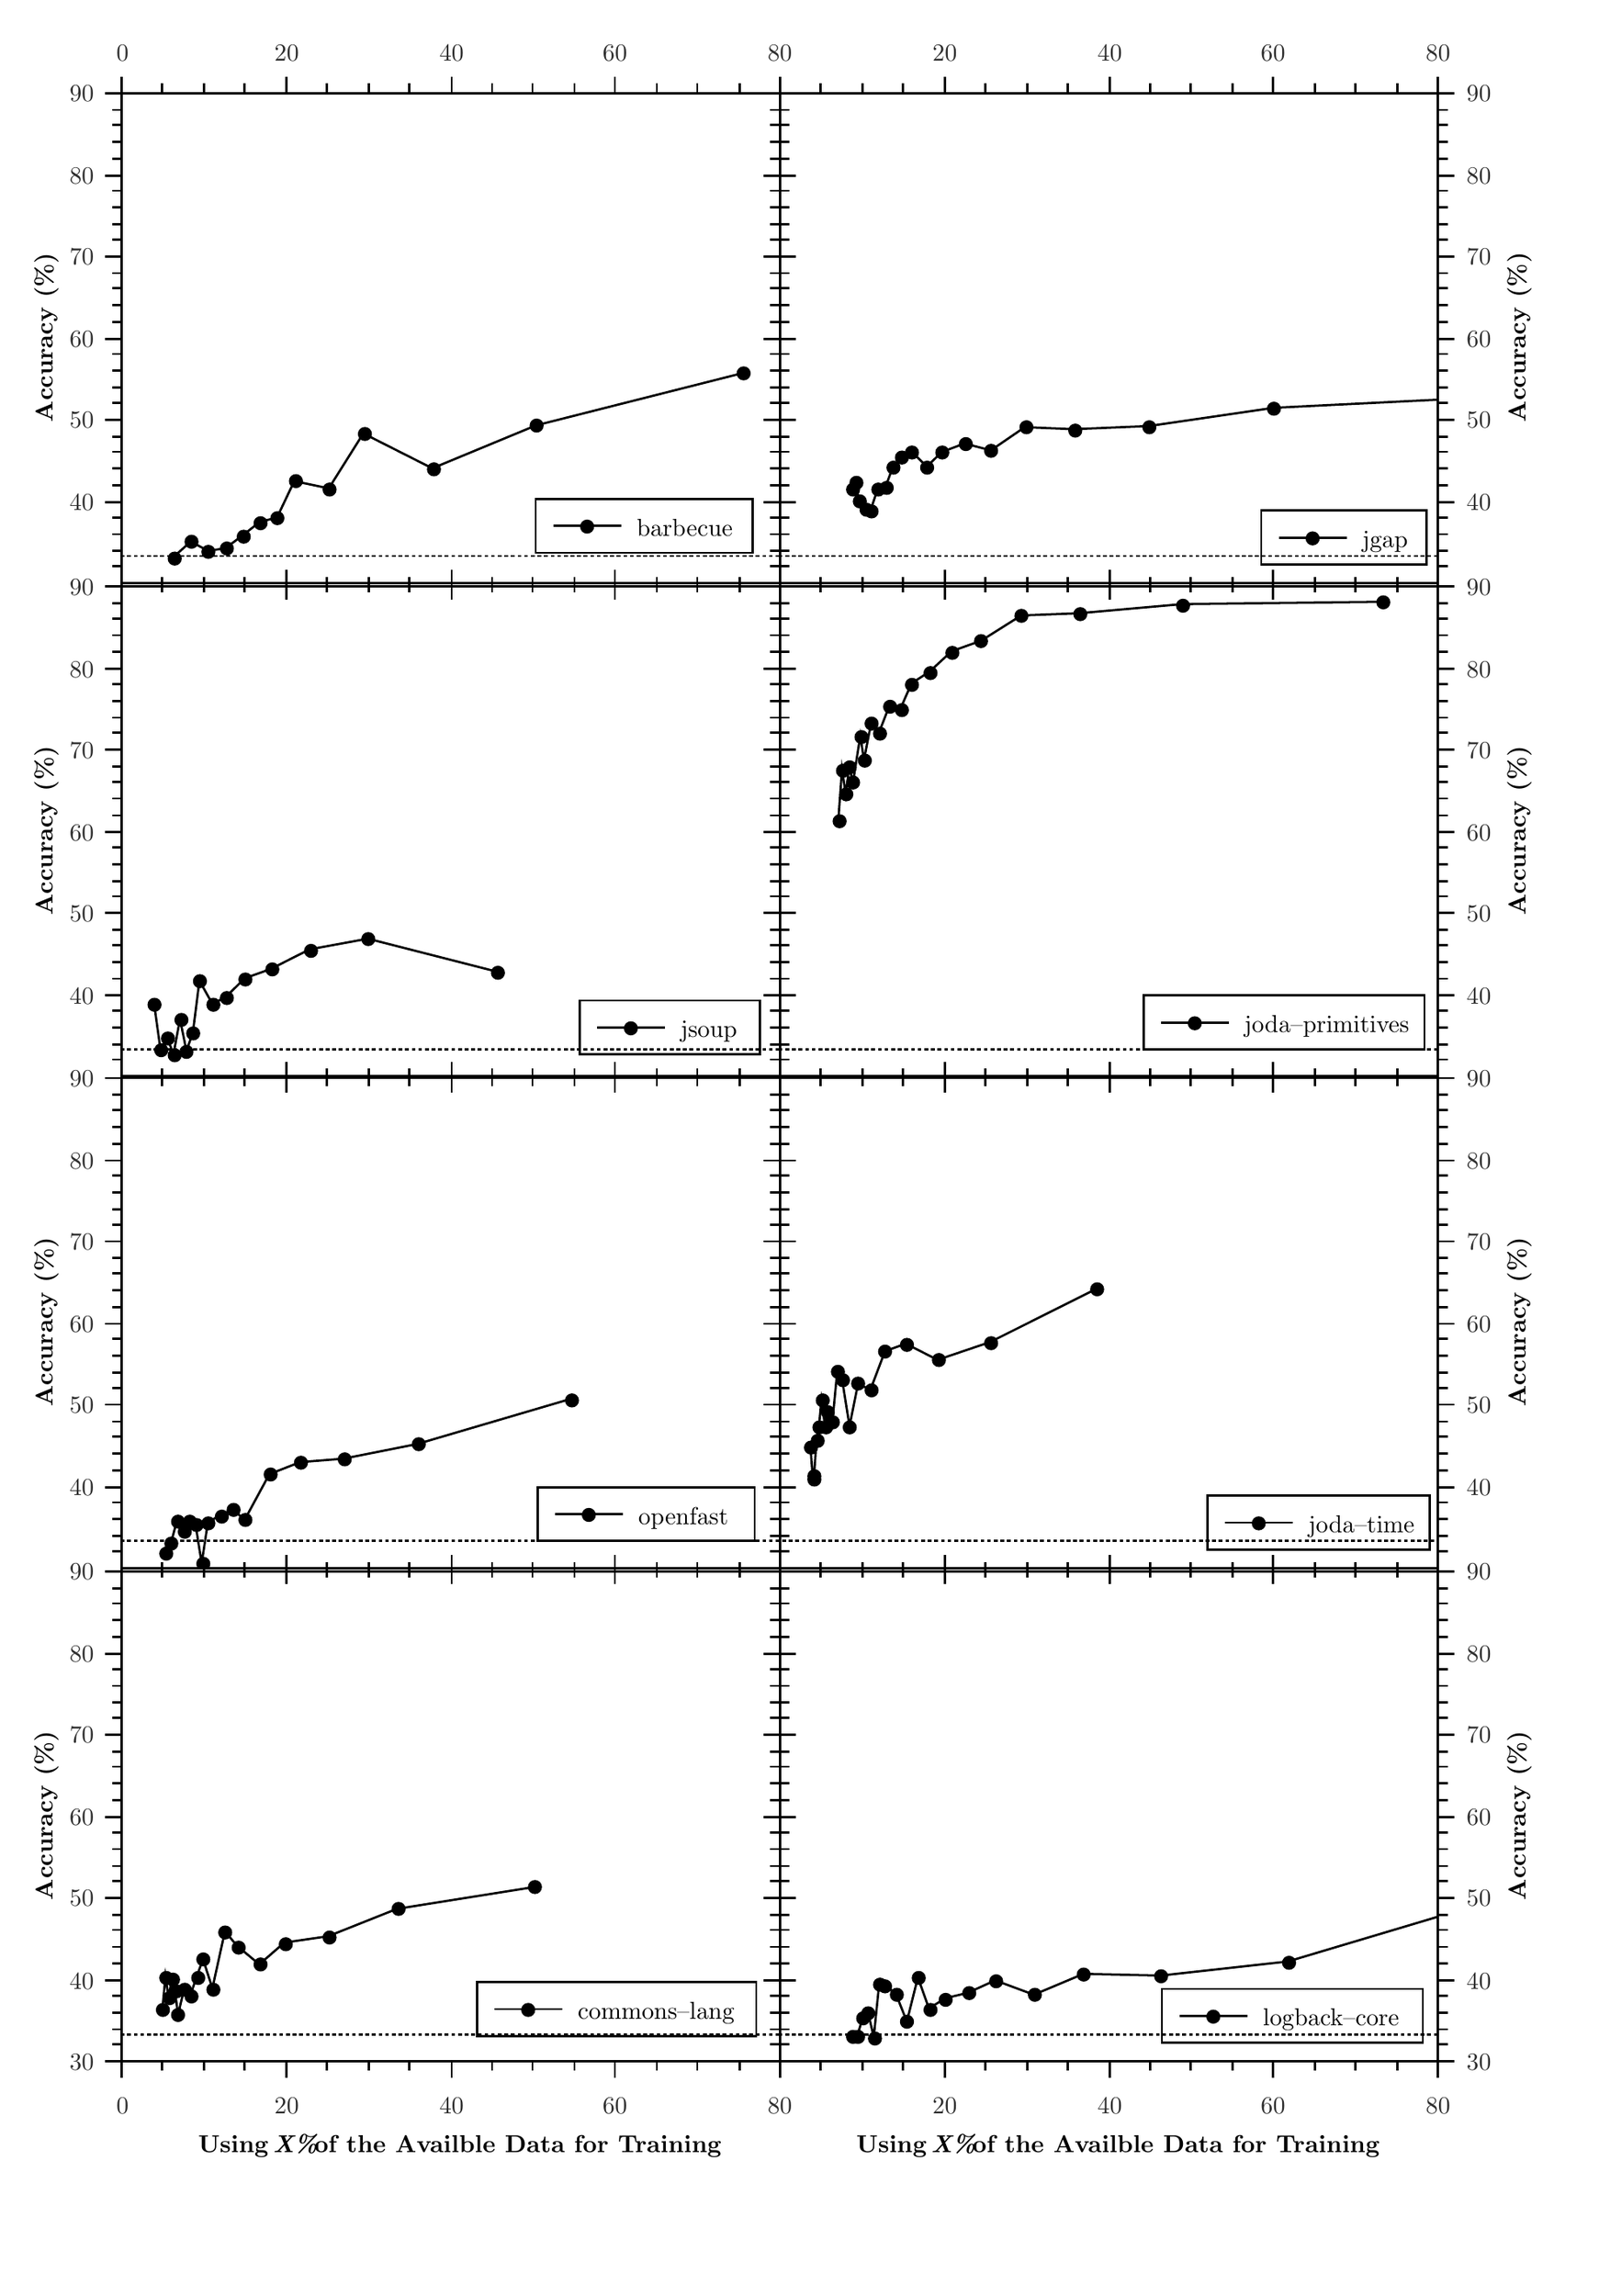
\begin{tikzpicture}{0pt}{0pt}{923pt}{1337pt}
	\clip(0pt,1337pt) -- (694.846pt,1337pt) -- (694.846pt,330.49pt) -- (0pt,330.49pt) -- (0pt,1337pt);
\begin{scope}
	\clip(44.4159pt,1305.38pt) -- (338.766pt,1305.38pt) -- (338.766pt,1086.31pt) -- (44.4159pt,1086.31pt) -- (44.4159pt,1305.38pt);
	\color[rgb]{0,0,0}
	\draw[line width=1pt, line join=miter, line cap=rect](322.299pt,1180.2pt) -- (229.671pt,1156.77pt) -- (183.357pt,1137.59pt) -- (152.481pt,1153.19pt) -- (137.043pt,1128.63pt) -- (121.606pt,1131.87pt) -- (113.887pt,1115.59pt) -- (106.168pt,1113.62pt) -- (98.4487pt,1107.56pt) -- (90.7297pt,1101.79pt) -- (83.0107pt,1100.72pt) -- (75.2918pt,1104.85pt) -- (67.5728pt,1097.89pt);
	\color[rgb]{0,0,0}
	\fill(322.58pt,1180.04pt) ellipse (2.63484pt and 2.63484pt);
	\draw[line width=1pt, line join=miter, line cap=rect](322.58pt,1180.04pt) ellipse (2.63484pt and 2.63484pt);
	\fill(229.984pt,1156.7pt) ellipse (2.63484pt and 2.63484pt);
	\draw[line width=1pt, line join=miter, line cap=rect](229.984pt,1156.7pt) ellipse (2.63484pt and 2.63484pt);
	\fill(184.063pt,1137.13pt) ellipse (2.63484pt and 2.63484pt);
	\draw[line width=1pt, line join=miter, line cap=rect](184.063pt,1137.13pt) ellipse (2.63484pt and 2.63484pt);
	\fill(153.197pt,1152.94pt) ellipse (2.63484pt and 2.63484pt);
	\draw[line width=1pt, line join=miter, line cap=rect](153.197pt,1152.94pt) ellipse (2.63484pt and 2.63484pt);
	\fill(137.388pt,1128.09pt) ellipse (2.63484pt and 2.63484pt);
	\draw[line width=1pt, line join=miter, line cap=rect](137.388pt,1128.09pt) ellipse (2.63484pt and 2.63484pt);
	\fill(122.332pt,1131.86pt) ellipse (2.63484pt and 2.63484pt);
	\draw[line width=1pt, line join=miter, line cap=rect](122.332pt,1131.86pt) ellipse (2.63484pt and 2.63484pt);
	\fill(114.051pt,1115.3pt) ellipse (2.63484pt and 2.63484pt);
	\draw[line width=1pt, line join=miter, line cap=rect](114.051pt,1115.3pt) ellipse (2.63484pt and 2.63484pt);
	\fill(106.523pt,1113.04pt) ellipse (2.63484pt and 2.63484pt);
	\draw[line width=1pt, line join=miter, line cap=rect](106.523pt,1113.04pt) ellipse (2.63484pt and 2.63484pt);
	\fill(98.9948pt,1107.02pt) ellipse (2.63484pt and 2.63484pt);
	\draw[line width=1pt, line join=miter, line cap=rect](98.9948pt,1107.02pt) ellipse (2.63484pt and 2.63484pt);
	\fill(91.4667pt,1101.75pt) ellipse (2.63484pt and 2.63484pt);
	\draw[line width=1pt, line join=miter, line cap=rect](91.4667pt,1101.75pt) ellipse (2.63484pt and 2.63484pt);
	\fill(83.1858pt,1100.24pt) ellipse (2.63484pt and 2.63484pt);
	\draw[line width=1pt, line join=miter, line cap=rect](83.1858pt,1100.24pt) ellipse (2.63484pt and 2.63484pt);
	\fill(75.6577pt,1104.76pt) ellipse (2.63484pt and 2.63484pt);
	\draw[line width=1pt, line join=miter, line cap=rect](75.6577pt,1104.76pt) ellipse (2.63484pt and 2.63484pt);
	\fill(68.1295pt,1097.23pt) ellipse (2.63484pt and 2.63484pt);
	\draw[line width=1pt, line join=miter, line cap=rect](68.1295pt,1097.23pt) ellipse (2.63484pt and 2.63484pt);
	\draw[line width=1pt, dash pattern=on 0.024cm off 0.08cm, dash phase=0pt, line join=miter, line cap=rect](44.4159pt,1098.36pt) -- (412.541pt,1098.36pt);
\end{scope}
\begin{scope}
	\color[rgb]{0,0,0}
	\pgftext[center, base, at={\pgfpoint{13.5506pt}{1196.22pt}},rotate=90]{\fontsize{11}{0}\selectfont{\textbf{Accuracy (\%)}}}
	\color[rgb]{0.172549,0.172549,0.172549}
	\pgftext[center, base, at={\pgfpoint{26.5719pt}{1118.68pt}}]{\fontsize{11}{0}\selectfont{40}}
	\pgftext[center, base, at={\pgfpoint{26.5719pt}{1155.57pt}}]{\fontsize{11}{0}\selectfont{50}}
	\pgftext[center, base, at={\pgfpoint{26.5719pt}{1191.71pt}}]{\fontsize{11}{0}\selectfont{60}}
	\pgftext[center, base, at={\pgfpoint{26.5719pt}{1228.6pt}}]{\fontsize{11}{0}\selectfont{70}}
	\pgftext[center, base, at={\pgfpoint{26.5719pt}{1264.73pt}}]{\fontsize{11}{0}\selectfont{80}}
	\pgftext[center, base, at={\pgfpoint{26.5719pt}{1301.62pt}}]{\fontsize{11}{0}\selectfont{90}}
	\color[rgb]{0,0,0}
	\draw[line width=1pt, line join=bevel, line cap=rect](44.4159pt,1093.84pt) -- (40.6519pt,1093.84pt);
	\draw[line width=1pt, line join=bevel, line cap=rect](44.4159pt,1100.62pt) -- (40.6519pt,1100.62pt);
	\draw[line width=1pt, line join=bevel, line cap=rect](44.4159pt,1108.14pt) -- (40.6519pt,1108.14pt);
	\draw[line width=1pt, line join=bevel, line cap=rect](44.4159pt,1115.67pt) -- (40.6519pt,1115.67pt);
	\draw[line width=1pt, line join=bevel, line cap=rect](44.4159pt,1129.98pt) -- (40.6519pt,1129.98pt);
	\draw[line width=1pt, line join=bevel, line cap=rect](44.4159pt,1137.5pt) -- (40.6519pt,1137.5pt);
	\draw[line width=1pt, line join=bevel, line cap=rect](44.4159pt,1145.03pt) -- (40.6519pt,1145.03pt);
	\draw[line width=1pt, line join=bevel, line cap=rect](44.4159pt,1151.81pt) -- (40.6519pt,1151.81pt);
	\draw[line width=1pt, line join=bevel, line cap=rect](44.4159pt,1166.86pt) -- (40.6519pt,1166.86pt);
	\draw[line width=1pt, line join=bevel, line cap=rect](44.4159pt,1173.64pt) -- (40.6519pt,1173.64pt);
	\draw[line width=1pt, line join=bevel, line cap=rect](44.4159pt,1181.17pt) -- (40.6519pt,1181.17pt);
	\draw[line width=1pt, line join=bevel, line cap=rect](44.4159pt,1188.7pt) -- (40.6519pt,1188.7pt);
	\draw[line width=1pt, line join=bevel, line cap=rect](44.4159pt,1203pt) -- (40.6519pt,1203pt);
	\draw[line width=1pt, line join=bevel, line cap=rect](44.4159pt,1210.53pt) -- (40.6519pt,1210.53pt);
	\draw[line width=1pt, line join=bevel, line cap=rect](44.4159pt,1218.06pt) -- (40.6519pt,1218.06pt);
	\draw[line width=1pt, line join=bevel, line cap=rect](44.4159pt,1224.83pt) -- (40.6519pt,1224.83pt);
	\draw[line width=1pt, line join=bevel, line cap=rect](44.4159pt,1239.89pt) -- (40.6519pt,1239.89pt);
	\draw[line width=1pt, line join=bevel, line cap=rect](44.4159pt,1246.66pt) -- (40.6519pt,1246.66pt);
	\draw[line width=1pt, line join=bevel, line cap=rect](44.4159pt,1254.19pt) -- (40.6519pt,1254.19pt);
	\draw[line width=1pt, line join=bevel, line cap=rect](44.4159pt,1261.72pt) -- (40.6519pt,1261.72pt);
	\draw[line width=1pt, line join=bevel, line cap=rect](44.4159pt,1276.02pt) -- (40.6519pt,1276.02pt);
	\draw[line width=1pt, line join=bevel, line cap=rect](44.4159pt,1283.55pt) -- (40.6519pt,1283.55pt);
	\draw[line width=1pt, line join=bevel, line cap=rect](44.4159pt,1291.08pt) -- (40.6519pt,1291.08pt);
	\draw[line width=1pt, line join=bevel, line cap=rect](44.4159pt,1297.85pt) -- (40.6519pt,1297.85pt);
	\draw[line width=1pt, line join=bevel, line cap=rect](44.4159pt,1122.45pt) -- (37.6406pt,1122.45pt);
	\draw[line width=1pt, line join=bevel, line cap=rect](44.4159pt,1159.34pt) -- (37.6406pt,1159.34pt);
	\draw[line width=1pt, line join=bevel, line cap=rect](44.4159pt,1195.47pt) -- (37.6406pt,1195.47pt);
	\draw[line width=1pt, line join=bevel, line cap=rect](44.4159pt,1232.36pt) -- (37.6406pt,1232.36pt);
	\draw[line width=1pt, line join=bevel, line cap=rect](44.4159pt,1268.49pt) -- (37.6406pt,1268.49pt);
	\draw[line width=1pt, line join=bevel, line cap=rect](44.4159pt,1305.38pt) -- (37.6406pt,1305.38pt);
	\draw[line width=1pt, line join=bevel, line cap=rect](44.4159pt,1305.38pt) -- (44.4159pt,1086.31pt);
	\draw[line width=1pt, line join=bevel, line cap=rect](338.766pt,1093.84pt) -- (342.53pt,1093.84pt);
	\draw[line width=1pt, line join=bevel, line cap=rect](338.766pt,1100.62pt) -- (342.53pt,1100.62pt);
	\draw[line width=1pt, line join=bevel, line cap=rect](338.766pt,1108.14pt) -- (342.53pt,1108.14pt);
	\draw[line width=1pt, line join=bevel, line cap=rect](338.766pt,1115.67pt) -- (342.53pt,1115.67pt);
	\draw[line width=1pt, line join=bevel, line cap=rect](338.766pt,1129.98pt) -- (342.53pt,1129.98pt);
	\draw[line width=1pt, line join=bevel, line cap=rect](338.766pt,1137.5pt) -- (342.53pt,1137.5pt);
	\draw[line width=1pt, line join=bevel, line cap=rect](338.766pt,1145.03pt) -- (342.53pt,1145.03pt);
	\draw[line width=1pt, line join=bevel, line cap=rect](338.766pt,1151.81pt) -- (342.53pt,1151.81pt);
	\draw[line width=1pt, line join=bevel, line cap=rect](338.766pt,1166.86pt) -- (342.53pt,1166.86pt);
	\draw[line width=1pt, line join=bevel, line cap=rect](338.766pt,1173.64pt) -- (342.53pt,1173.64pt);
	\draw[line width=1pt, line join=bevel, line cap=rect](338.766pt,1181.17pt) -- (342.53pt,1181.17pt);
	\draw[line width=1pt, line join=bevel, line cap=rect](338.766pt,1188.7pt) -- (342.53pt,1188.7pt);
	\draw[line width=1pt, line join=bevel, line cap=rect](338.766pt,1203pt) -- (342.53pt,1203pt);
	\draw[line width=1pt, line join=bevel, line cap=rect](338.766pt,1210.53pt) -- (342.53pt,1210.53pt);
	\draw[line width=1pt, line join=bevel, line cap=rect](338.766pt,1218.06pt) -- (342.53pt,1218.06pt);
	\draw[line width=1pt, line join=bevel, line cap=rect](338.766pt,1224.83pt) -- (342.53pt,1224.83pt);
	\draw[line width=1pt, line join=bevel, line cap=rect](338.766pt,1239.89pt) -- (342.53pt,1239.89pt);
	\draw[line width=1pt, line join=bevel, line cap=rect](338.766pt,1246.66pt) -- (342.53pt,1246.66pt);
	\draw[line width=1pt, line join=bevel, line cap=rect](338.766pt,1254.19pt) -- (342.53pt,1254.19pt);
	\draw[line width=1pt, line join=bevel, line cap=rect](338.766pt,1261.72pt) -- (342.53pt,1261.72pt);
	\draw[line width=1pt, line join=bevel, line cap=rect](338.766pt,1276.02pt) -- (342.53pt,1276.02pt);
	\draw[line width=1pt, line join=bevel, line cap=rect](338.766pt,1283.55pt) -- (342.53pt,1283.55pt);
	\draw[line width=1pt, line join=bevel, line cap=rect](338.766pt,1291.08pt) -- (342.53pt,1291.08pt);
	\draw[line width=1pt, line join=bevel, line cap=rect](338.766pt,1297.85pt) -- (342.53pt,1297.85pt);
	\draw[line width=1pt, line join=bevel, line cap=rect](338.766pt,1086.31pt) -- (345.541pt,1086.31pt);
	\draw[line width=1pt, line join=bevel, line cap=rect](338.766pt,1122.45pt) -- (345.541pt,1122.45pt);
	\draw[line width=1pt, line join=bevel, line cap=rect](338.766pt,1159.34pt) -- (345.541pt,1159.34pt);
	\draw[line width=1pt, line join=bevel, line cap=rect](338.766pt,1195.47pt) -- (345.541pt,1195.47pt);
	\draw[line width=1pt, line join=bevel, line cap=rect](338.766pt,1232.36pt) -- (345.541pt,1232.36pt);
	\draw[line width=1pt, line join=bevel, line cap=rect](338.766pt,1268.49pt) -- (345.541pt,1268.49pt);
	\draw[line width=1pt, line join=bevel, line cap=rect](338.766pt,1305.38pt) -- (345.541pt,1305.38pt);
	\draw[line width=1pt, line join=bevel, line cap=rect](338.766pt,1305.38pt) -- (338.766pt,1086.31pt);
	\draw[line width=1pt, line join=bevel, line cap=rect](62.4834pt,1086.31pt) -- (62.4834pt,1082.55pt);
	\draw[line width=1pt, line join=bevel, line cap=rect](99.3713pt,1086.31pt) -- (99.3713pt,1082.55pt);
	\draw[line width=1pt, line join=bevel, line cap=rect](136.259pt,1086.31pt) -- (136.259pt,1082.55pt);
	\draw[line width=1pt, line join=bevel, line cap=rect](173.147pt,1086.31pt) -- (173.147pt,1082.55pt);
	\draw[line width=1pt, line join=bevel, line cap=rect](210.035pt,1086.31pt) -- (210.035pt,1082.55pt);
	\draw[line width=1pt, line join=bevel, line cap=rect](246.922pt,1086.31pt) -- (246.922pt,1082.55pt);
	\draw[line width=1pt, line join=bevel, line cap=rect](283.81pt,1086.31pt) -- (283.81pt,1082.55pt);
	\draw[line width=1pt, line join=bevel, line cap=rect](320.698pt,1086.31pt) -- (320.698pt,1082.55pt);
	\draw[line width=1pt, line join=bevel, line cap=rect](81.3037pt,1086.31pt) -- (81.3037pt,1082.55pt);
	\draw[line width=1pt, line join=bevel, line cap=rect](155.079pt,1086.31pt) -- (155.079pt,1082.55pt);
	\draw[line width=1pt, line join=bevel, line cap=rect](228.102pt,1086.31pt) -- (228.102pt,1082.55pt);
	\draw[line width=1pt, line join=bevel, line cap=rect](301.878pt,1086.31pt) -- (301.878pt,1082.55pt);
	\draw[line width=1pt, line join=bevel, line cap=rect](44.4159pt,1086.31pt) -- (44.4159pt,1079.54pt);
	\draw[line width=1pt, line join=bevel, line cap=rect](118.192pt,1086.31pt) -- (118.192pt,1079.54pt);
	\draw[line width=1pt, line join=bevel, line cap=rect](191.967pt,1086.31pt) -- (191.967pt,1079.54pt);
	\draw[line width=1pt, line join=bevel, line cap=rect](264.99pt,1086.31pt) -- (264.99pt,1079.54pt);
	\draw[line width=1pt, line join=bevel, line cap=rect](338.766pt,1086.31pt) -- (338.766pt,1079.54pt);
	\draw[line width=1pt, line join=bevel, line cap=rect](44.4159pt,1086.31pt) -- (338.766pt,1086.31pt);
	\color[rgb]{0.172549,0.172549,0.172549}
	\pgftext[center, base, at={\pgfpoint{44.7865pt}{1319.69pt}}]{\fontsize{11}{0}\selectfont{0}}
	\pgftext[center, base, at={\pgfpoint{118.192pt}{1319.69pt}}]{\fontsize{11}{0}\selectfont{20}}
	\pgftext[center, base, at={\pgfpoint{191.967pt}{1319.69pt}}]{\fontsize{11}{0}\selectfont{40}}
	\pgftext[center, base, at={\pgfpoint{264.99pt}{1319.69pt}}]{\fontsize{11}{0}\selectfont{60}}
	\pgftext[center, base, at={\pgfpoint{338.766pt}{1319.69pt}}]{\fontsize{11}{0}\selectfont{80}}
	\color[rgb]{0,0,0}
	\draw[line width=1pt, line join=bevel, line cap=rect](62.4834pt,1305.38pt) -- (62.4834pt,1309.15pt);
	\draw[line width=1pt, line join=bevel, line cap=rect](99.3713pt,1305.38pt) -- (99.3713pt,1309.15pt);
	\draw[line width=1pt, line join=bevel, line cap=rect](136.259pt,1305.38pt) -- (136.259pt,1309.15pt);
	\draw[line width=1pt, line join=bevel, line cap=rect](173.147pt,1305.38pt) -- (173.147pt,1309.15pt);
	\draw[line width=1pt, line join=bevel, line cap=rect](210.035pt,1305.38pt) -- (210.035pt,1309.15pt);
	\draw[line width=1pt, line join=bevel, line cap=rect](246.922pt,1305.38pt) -- (246.922pt,1309.15pt);
	\draw[line width=1pt, line join=bevel, line cap=rect](283.81pt,1305.38pt) -- (283.81pt,1309.15pt);
	\draw[line width=1pt, line join=bevel, line cap=rect](320.698pt,1305.38pt) -- (320.698pt,1309.15pt);
	\draw[line width=1pt, line join=bevel, line cap=rect](81.3037pt,1305.38pt) -- (81.3037pt,1309.15pt);
	\draw[line width=1pt, line join=bevel, line cap=rect](155.079pt,1305.38pt) -- (155.079pt,1309.15pt);
	\draw[line width=1pt, line join=bevel, line cap=rect](228.102pt,1305.38pt) -- (228.102pt,1309.15pt);
	\draw[line width=1pt, line join=bevel, line cap=rect](301.878pt,1305.38pt) -- (301.878pt,1309.15pt);
	\draw[line width=1pt, line join=bevel, line cap=rect](44.4159pt,1305.38pt) -- (44.4159pt,1312.16pt);
	\draw[line width=1pt, line join=bevel, line cap=rect](118.192pt,1305.38pt) -- (118.192pt,1312.16pt);
	\draw[line width=1pt, line join=bevel, line cap=rect](191.967pt,1305.38pt) -- (191.967pt,1312.16pt);
	\draw[line width=1pt, line join=bevel, line cap=rect](264.99pt,1305.38pt) -- (264.99pt,1312.16pt);
	\draw[line width=1pt, line join=bevel, line cap=rect](338.766pt,1305.38pt) -- (338.766pt,1312.16pt);
	\draw[line width=1pt, line join=bevel, line cap=rect](44.4159pt,1305.38pt) -- (338.766pt,1305.38pt);
	\draw[line width=1pt, line join=miter, line cap=rect](229.608pt,1123.95pt) -- (326.721pt,1123.95pt) -- (326.721pt,1099.86pt) -- (229.608pt,1099.86pt) -- (229.608pt,1123.95pt);
	\draw[line width=1pt, line join=miter, line cap=rect](237.889pt,1111.91pt) -- (267.248pt,1111.91pt);
	\fill(252.569pt,1111.53pt) ellipse (2.63484pt and 2.63484pt);
	\draw[line width=1pt, line join=miter, line cap=rect](252.569pt,1111.53pt) ellipse (2.63484pt and 2.63484pt);
	\pgftext[left, base, at={\pgfpoint{274.777pt}{1107.39pt}}]{\fontsize{11}{0}\selectfont{barbecue}}
\end{scope}
\begin{scope}
	\clip(44.4159pt,1084.81pt) -- (338.766pt,1084.81pt) -- (338.766pt,865.739pt) -- (44.4159pt,865.739pt) -- (44.4159pt,1084.81pt);
	\color[rgb]{0,0,0}
	\draw[line width=1pt, line join=miter, line cap=rect](212.45pt,912.481pt) -- (154.507pt,927.275pt) -- (128.433pt,922.493pt) -- (111.05pt,913.719pt) -- (99.4616pt,909.576pt) -- (90.7702pt,901.045pt) -- (84.9759pt,898.158pt) -- (79.1816pt,908.495pt) -- (76.2845pt,885.464pt) -- (73.3874pt,877.078pt) -- (70.4902pt,891.318pt) -- (67.5931pt,875.711pt) -- (64.6959pt,883.082pt) -- (61.7988pt,877.44pt) -- (58.9017pt,898.26pt);
	\color[rgb]{0,0,0}
	\fill(212.67pt,912.037pt) ellipse (2.63484pt and 2.63484pt);
	\draw[line width=1pt, line join=miter, line cap=rect](212.67pt,912.037pt) ellipse (2.63484pt and 2.63484pt);
	\fill(154.703pt,927.094pt) ellipse (2.63484pt and 2.63484pt);
	\draw[line width=1pt, line join=miter, line cap=rect](154.703pt,927.094pt) ellipse (2.63484pt and 2.63484pt);
	\fill(129.107pt,921.824pt) ellipse (2.63484pt and 2.63484pt);
	\draw[line width=1pt, line join=miter, line cap=rect](129.107pt,921.824pt) ellipse (2.63484pt and 2.63484pt);
	\fill(111.793pt,913.543pt) ellipse (2.63484pt and 2.63484pt);
	\draw[line width=1pt, line join=miter, line cap=rect](111.793pt,913.543pt) ellipse (2.63484pt and 2.63484pt);
	\fill(99.7477pt,909.026pt) ellipse (2.63484pt and 2.63484pt);
	\draw[line width=1pt, line join=miter, line cap=rect](99.7477pt,909.026pt) ellipse (2.63484pt and 2.63484pt);
	\fill(91.4667pt,900.745pt) ellipse (2.63484pt and 2.63484pt);
	\draw[line width=1pt, line join=miter, line cap=rect](91.4667pt,900.745pt) ellipse (2.63484pt and 2.63484pt);
	\fill(85.4442pt,897.734pt) ellipse (2.63484pt and 2.63484pt);
	\draw[line width=1pt, line join=miter, line cap=rect](85.4442pt,897.734pt) ellipse (2.63484pt and 2.63484pt);
	\fill(79.4217pt,908.273pt) ellipse (2.63484pt and 2.63484pt);
	\draw[line width=1pt, line join=miter, line cap=rect](79.4217pt,908.273pt) ellipse (2.63484pt and 2.63484pt);
	\fill(76.4105pt,884.936pt) ellipse (2.63484pt and 2.63484pt);
	\draw[line width=1pt, line join=miter, line cap=rect](76.4105pt,884.936pt) ellipse (2.63484pt and 2.63484pt);
	\fill(73.3992pt,876.655pt) ellipse (2.63484pt and 2.63484pt);
	\draw[line width=1pt, line join=miter, line cap=rect](73.3992pt,876.655pt) ellipse (2.63484pt and 2.63484pt);
	\fill(71.1408pt,890.959pt) ellipse (2.63484pt and 2.63484pt);
	\draw[line width=1pt, line join=miter, line cap=rect](71.1408pt,890.959pt) ellipse (2.63484pt and 2.63484pt);
	\fill(68.1295pt,875.15pt) ellipse (2.63484pt and 2.63484pt);
	\draw[line width=1pt, line join=miter, line cap=rect](68.1295pt,875.15pt) ellipse (2.63484pt and 2.63484pt);
	\fill(65.1183pt,882.678pt) ellipse (2.63484pt and 2.63484pt);
	\draw[line width=1pt, line join=miter, line cap=rect](65.1183pt,882.678pt) ellipse (2.63484pt and 2.63484pt);
	\fill(62.107pt,877.408pt) ellipse (2.63484pt and 2.63484pt);
	\draw[line width=1pt, line join=miter, line cap=rect](62.107pt,877.408pt) ellipse (2.63484pt and 2.63484pt);
	\fill(59.0958pt,897.734pt) ellipse (2.63484pt and 2.63484pt);
	\draw[line width=1pt, line join=miter, line cap=rect](59.0958pt,897.734pt) ellipse (2.63484pt and 2.63484pt);
	\draw[line width=1pt, dash pattern=on 0.024cm off 0.08cm, dash phase=0pt, line join=miter, line cap=rect](44.4159pt,877.784pt) -- (412.541pt,877.784pt);
\end{scope}
\begin{scope}
	\color[rgb]{0,0,0}
	\pgftext[center, base, at={\pgfpoint{13.5506pt}{975.644pt}},rotate=90]{\fontsize{11}{0}\selectfont{\textbf{Accuracy (\%)}}}
	\color[rgb]{0.172549,0.172549,0.172549}
	\pgftext[center, base, at={\pgfpoint{26.5719pt}{898.11pt}}]{\fontsize{11}{0}\selectfont{40}}
	\pgftext[center, base, at={\pgfpoint{26.5719pt}{934.998pt}}]{\fontsize{11}{0}\selectfont{50}}
	\pgftext[center, base, at={\pgfpoint{26.5719pt}{971.133pt}}]{\fontsize{11}{0}\selectfont{60}}
	\pgftext[center, base, at={\pgfpoint{26.5719pt}{1008.02pt}}]{\fontsize{11}{0}\selectfont{70}}
	\pgftext[center, base, at={\pgfpoint{26.5719pt}{1044.16pt}}]{\fontsize{11}{0}\selectfont{80}}
	\pgftext[center, base, at={\pgfpoint{26.5719pt}{1081.04pt}}]{\fontsize{11}{0}\selectfont{90}}
	\color[rgb]{0,0,0}
	\draw[line width=1pt, line join=bevel, line cap=rect](44.4159pt,873.267pt) -- (40.6519pt,873.267pt);
	\draw[line width=1pt, line join=bevel, line cap=rect](44.4159pt,880.043pt) -- (40.6519pt,880.043pt);
	\draw[line width=1pt, line join=bevel, line cap=rect](44.4159pt,887.571pt) -- (40.6519pt,887.571pt);
	\draw[line width=1pt, line join=bevel, line cap=rect](44.4159pt,895.099pt) -- (40.6519pt,895.099pt);
	\draw[line width=1pt, line join=bevel, line cap=rect](44.4159pt,909.402pt) -- (40.6519pt,909.402pt);
	\draw[line width=1pt, line join=bevel, line cap=rect](44.4159pt,916.931pt) -- (40.6519pt,916.931pt);
	\draw[line width=1pt, line join=bevel, line cap=rect](44.4159pt,924.459pt) -- (40.6519pt,924.459pt);
	\draw[line width=1pt, line join=bevel, line cap=rect](44.4159pt,931.234pt) -- (40.6519pt,931.234pt);
	\draw[line width=1pt, line join=bevel, line cap=rect](44.4159pt,946.29pt) -- (40.6519pt,946.29pt);
	\draw[line width=1pt, line join=bevel, line cap=rect](44.4159pt,953.066pt) -- (40.6519pt,953.066pt);
	\draw[line width=1pt, line join=bevel, line cap=rect](44.4159pt,960.594pt) -- (40.6519pt,960.594pt);
	\draw[line width=1pt, line join=bevel, line cap=rect](44.4159pt,968.122pt) -- (40.6519pt,968.122pt);
	\draw[line width=1pt, line join=bevel, line cap=rect](44.4159pt,982.425pt) -- (40.6519pt,982.425pt);
	\draw[line width=1pt, line join=bevel, line cap=rect](44.4159pt,989.953pt) -- (40.6519pt,989.953pt);
	\draw[line width=1pt, line join=bevel, line cap=rect](44.4159pt,997.482pt) -- (40.6519pt,997.482pt);
	\draw[line width=1pt, line join=bevel, line cap=rect](44.4159pt,1004.26pt) -- (40.6519pt,1004.26pt);
	\draw[line width=1pt, line join=bevel, line cap=rect](44.4159pt,1019.31pt) -- (40.6519pt,1019.31pt);
	\draw[line width=1pt, line join=bevel, line cap=rect](44.4159pt,1026.09pt) -- (40.6519pt,1026.09pt);
	\draw[line width=1pt, line join=bevel, line cap=rect](44.4159pt,1033.62pt) -- (40.6519pt,1033.62pt);
	\draw[line width=1pt, line join=bevel, line cap=rect](44.4159pt,1041.14pt) -- (40.6519pt,1041.14pt);
	\draw[line width=1pt, line join=bevel, line cap=rect](44.4159pt,1055.45pt) -- (40.6519pt,1055.45pt);
	\draw[line width=1pt, line join=bevel, line cap=rect](44.4159pt,1062.98pt) -- (40.6519pt,1062.98pt);
	\draw[line width=1pt, line join=bevel, line cap=rect](44.4159pt,1070.5pt) -- (40.6519pt,1070.5pt);
	\draw[line width=1pt, line join=bevel, line cap=rect](44.4159pt,1077.28pt) -- (40.6519pt,1077.28pt);
	\draw[line width=1pt, line join=bevel, line cap=rect](44.4159pt,901.874pt) -- (37.6406pt,901.874pt);
	\draw[line width=1pt, line join=bevel, line cap=rect](44.4159pt,938.762pt) -- (37.6406pt,938.762pt);
	\draw[line width=1pt, line join=bevel, line cap=rect](44.4159pt,974.897pt) -- (37.6406pt,974.897pt);
	\draw[line width=1pt, line join=bevel, line cap=rect](44.4159pt,1011.79pt) -- (37.6406pt,1011.79pt);
	\draw[line width=1pt, line join=bevel, line cap=rect](44.4159pt,1047.92pt) -- (37.6406pt,1047.92pt);
	\draw[line width=1pt, line join=bevel, line cap=rect](44.4159pt,1084.81pt) -- (37.6406pt,1084.81pt);
	\draw[line width=1pt, line join=bevel, line cap=rect](44.4159pt,1084.81pt) -- (44.4159pt,865.739pt);
	\draw[line width=1pt, line join=bevel, line cap=rect](338.766pt,873.267pt) -- (342.53pt,873.267pt);
	\draw[line width=1pt, line join=bevel, line cap=rect](338.766pt,880.043pt) -- (342.53pt,880.043pt);
	\draw[line width=1pt, line join=bevel, line cap=rect](338.766pt,887.571pt) -- (342.53pt,887.571pt);
	\draw[line width=1pt, line join=bevel, line cap=rect](338.766pt,895.099pt) -- (342.53pt,895.099pt);
	\draw[line width=1pt, line join=bevel, line cap=rect](338.766pt,909.402pt) -- (342.53pt,909.402pt);
	\draw[line width=1pt, line join=bevel, line cap=rect](338.766pt,916.931pt) -- (342.53pt,916.931pt);
	\draw[line width=1pt, line join=bevel, line cap=rect](338.766pt,924.459pt) -- (342.53pt,924.459pt);
	\draw[line width=1pt, line join=bevel, line cap=rect](338.766pt,931.234pt) -- (342.53pt,931.234pt);
	\draw[line width=1pt, line join=bevel, line cap=rect](338.766pt,946.29pt) -- (342.53pt,946.29pt);
	\draw[line width=1pt, line join=bevel, line cap=rect](338.766pt,953.066pt) -- (342.53pt,953.066pt);
	\draw[line width=1pt, line join=bevel, line cap=rect](338.766pt,960.594pt) -- (342.53pt,960.594pt);
	\draw[line width=1pt, line join=bevel, line cap=rect](338.766pt,968.122pt) -- (342.53pt,968.122pt);
	\draw[line width=1pt, line join=bevel, line cap=rect](338.766pt,982.425pt) -- (342.53pt,982.425pt);
	\draw[line width=1pt, line join=bevel, line cap=rect](338.766pt,989.953pt) -- (342.53pt,989.953pt);
	\draw[line width=1pt, line join=bevel, line cap=rect](338.766pt,997.482pt) -- (342.53pt,997.482pt);
	\draw[line width=1pt, line join=bevel, line cap=rect](338.766pt,1004.26pt) -- (342.53pt,1004.26pt);
	\draw[line width=1pt, line join=bevel, line cap=rect](338.766pt,1019.31pt) -- (342.53pt,1019.31pt);
	\draw[line width=1pt, line join=bevel, line cap=rect](338.766pt,1026.09pt) -- (342.53pt,1026.09pt);
	\draw[line width=1pt, line join=bevel, line cap=rect](338.766pt,1033.62pt) -- (342.53pt,1033.62pt);
	\draw[line width=1pt, line join=bevel, line cap=rect](338.766pt,1041.14pt) -- (342.53pt,1041.14pt);
	\draw[line width=1pt, line join=bevel, line cap=rect](338.766pt,1055.45pt) -- (342.53pt,1055.45pt);
	\draw[line width=1pt, line join=bevel, line cap=rect](338.766pt,1062.98pt) -- (342.53pt,1062.98pt);
	\draw[line width=1pt, line join=bevel, line cap=rect](338.766pt,1070.5pt) -- (342.53pt,1070.5pt);
	\draw[line width=1pt, line join=bevel, line cap=rect](338.766pt,1077.28pt) -- (342.53pt,1077.28pt);
	\draw[line width=1pt, line join=bevel, line cap=rect](338.766pt,865.739pt) -- (345.541pt,865.739pt);
	\draw[line width=1pt, line join=bevel, line cap=rect](338.766pt,901.874pt) -- (345.541pt,901.874pt);
	\draw[line width=1pt, line join=bevel, line cap=rect](338.766pt,938.762pt) -- (345.541pt,938.762pt);
	\draw[line width=1pt, line join=bevel, line cap=rect](338.766pt,974.897pt) -- (345.541pt,974.897pt);
	\draw[line width=1pt, line join=bevel, line cap=rect](338.766pt,1011.79pt) -- (345.541pt,1011.79pt);
	\draw[line width=1pt, line join=bevel, line cap=rect](338.766pt,1047.92pt) -- (345.541pt,1047.92pt);
	\draw[line width=1pt, line join=bevel, line cap=rect](338.766pt,1084.81pt) -- (345.541pt,1084.81pt);
	\draw[line width=1pt, line join=bevel, line cap=rect](338.766pt,1084.81pt) -- (338.766pt,865.739pt);
	\draw[line width=1pt, line join=bevel, line cap=rect](62.4834pt,865.739pt) -- (62.4834pt,861.975pt);
	\draw[line width=1pt, line join=bevel, line cap=rect](99.3713pt,865.739pt) -- (99.3713pt,861.975pt);
	\draw[line width=1pt, line join=bevel, line cap=rect](136.259pt,865.739pt) -- (136.259pt,861.975pt);
	\draw[line width=1pt, line join=bevel, line cap=rect](173.147pt,865.739pt) -- (173.147pt,861.975pt);
	\draw[line width=1pt, line join=bevel, line cap=rect](210.035pt,865.739pt) -- (210.035pt,861.975pt);
	\draw[line width=1pt, line join=bevel, line cap=rect](246.922pt,865.739pt) -- (246.922pt,861.975pt);
	\draw[line width=1pt, line join=bevel, line cap=rect](283.81pt,865.739pt) -- (283.81pt,861.975pt);
	\draw[line width=1pt, line join=bevel, line cap=rect](320.698pt,865.739pt) -- (320.698pt,861.975pt);
	\draw[line width=1pt, line join=bevel, line cap=rect](81.3037pt,865.739pt) -- (81.3037pt,861.975pt);
	\draw[line width=1pt, line join=bevel, line cap=rect](155.079pt,865.739pt) -- (155.079pt,861.975pt);
	\draw[line width=1pt, line join=bevel, line cap=rect](228.102pt,865.739pt) -- (228.102pt,861.975pt);
	\draw[line width=1pt, line join=bevel, line cap=rect](301.878pt,865.739pt) -- (301.878pt,861.975pt);
	\draw[line width=1pt, line join=bevel, line cap=rect](44.4159pt,865.739pt) -- (44.4159pt,858.964pt);
	\draw[line width=1pt, line join=bevel, line cap=rect](118.192pt,865.739pt) -- (118.192pt,858.964pt);
	\draw[line width=1pt, line join=bevel, line cap=rect](191.967pt,865.739pt) -- (191.967pt,858.964pt);
	\draw[line width=1pt, line join=bevel, line cap=rect](264.99pt,865.739pt) -- (264.99pt,858.964pt);
	\draw[line width=1pt, line join=bevel, line cap=rect](338.766pt,865.739pt) -- (338.766pt,858.964pt);
	\draw[line width=1pt, line join=bevel, line cap=rect](44.4159pt,865.739pt) -- (338.766pt,865.739pt);
	\draw[line width=1pt, line join=bevel, line cap=rect](62.4834pt,1084.81pt) -- (62.4834pt,1088.57pt);
	\draw[line width=1pt, line join=bevel, line cap=rect](99.3713pt,1084.81pt) -- (99.3713pt,1088.57pt);
	\draw[line width=1pt, line join=bevel, line cap=rect](136.259pt,1084.81pt) -- (136.259pt,1088.57pt);
	\draw[line width=1pt, line join=bevel, line cap=rect](173.147pt,1084.81pt) -- (173.147pt,1088.57pt);
	\draw[line width=1pt, line join=bevel, line cap=rect](210.035pt,1084.81pt) -- (210.035pt,1088.57pt);
	\draw[line width=1pt, line join=bevel, line cap=rect](246.922pt,1084.81pt) -- (246.922pt,1088.57pt);
	\draw[line width=1pt, line join=bevel, line cap=rect](283.81pt,1084.81pt) -- (283.81pt,1088.57pt);
	\draw[line width=1pt, line join=bevel, line cap=rect](320.698pt,1084.81pt) -- (320.698pt,1088.57pt);
	\draw[line width=1pt, line join=bevel, line cap=rect](81.3037pt,1084.81pt) -- (81.3037pt,1088.57pt);
	\draw[line width=1pt, line join=bevel, line cap=rect](155.079pt,1084.81pt) -- (155.079pt,1088.57pt);
	\draw[line width=1pt, line join=bevel, line cap=rect](228.102pt,1084.81pt) -- (228.102pt,1088.57pt);
	\draw[line width=1pt, line join=bevel, line cap=rect](301.878pt,1084.81pt) -- (301.878pt,1088.57pt);
	\draw[line width=1pt, line join=bevel, line cap=rect](44.4159pt,1084.81pt) -- (44.4159pt,1091.58pt);
	\draw[line width=1pt, line join=bevel, line cap=rect](118.192pt,1084.81pt) -- (118.192pt,1091.58pt);
	\draw[line width=1pt, line join=bevel, line cap=rect](191.967pt,1084.81pt) -- (191.967pt,1091.58pt);
	\draw[line width=1pt, line join=bevel, line cap=rect](264.99pt,1084.81pt) -- (264.99pt,1091.58pt);
	\draw[line width=1pt, line join=bevel, line cap=rect](338.766pt,1084.81pt) -- (338.766pt,1091.58pt);
	\draw[line width=1pt, line join=bevel, line cap=rect](44.4159pt,1084.81pt) -- (338.766pt,1084.81pt);
	\draw[line width=1pt, line join=miter, line cap=rect](249.181pt,899.616pt) -- (329.732pt,899.616pt) -- (329.732pt,875.526pt) -- (249.181pt,875.526pt) -- (249.181pt,899.616pt);
	\draw[line width=1pt, line join=miter, line cap=rect](257.462pt,887.571pt) -- (286.822pt,887.571pt);
	\fill(272.142pt,887.195pt) ellipse (2.63484pt and 2.63484pt);
	\draw[line width=1pt, line join=miter, line cap=rect](272.142pt,887.195pt) ellipse (2.63484pt and 2.63484pt);
	\pgftext[left, base, at={\pgfpoint{294.35pt}{883.054pt}}]{\fontsize{11}{0}\selectfont{jsoup}}
\end{scope}
\begin{scope}
	\clip(44.4159pt,864.987pt) -- (338.766pt,864.987pt) -- (338.766pt,645.918pt) -- (44.4159pt,645.918pt) -- (44.4159pt,864.987pt);
	\color[rgb]{0,0,0}
	\draw[line width=1pt, line join=miter, line cap=rect](245.359pt,721.549pt) -- (176.543pt,701.325pt) -- (143.511pt,694.766pt) -- (124.243pt,693.243pt) -- (110.479pt,687.867pt) -- (99.4689pt,667.547pt) -- (93.9636pt,672.013pt) -- (88.4583pt,669.604pt) -- (82.953pt,666.157pt) -- (80.2003pt,648.036pt) -- (77.4477pt,665.224pt) -- (74.6951pt,667.25pt) -- (71.9424pt,662.255pt) -- (69.1898pt,667.298pt) -- (66.4371pt,656.959pt) -- (63.6845pt,652.93pt);
	\color[rgb]{0,0,0}
	\fill(245.793pt,720.823pt) ellipse (2.63484pt and 2.63484pt);
	\draw[line width=1pt, line join=miter, line cap=rect](245.793pt,720.823pt) ellipse (2.63484pt and 2.63484pt);
	\fill(177.287pt,701.25pt) ellipse (2.63484pt and 2.63484pt);
	\draw[line width=1pt, line join=miter, line cap=rect](177.287pt,701.25pt) ellipse (2.63484pt and 2.63484pt);
	\fill(144.164pt,694.475pt) ellipse (2.63484pt and 2.63484pt);
	\draw[line width=1pt, line join=miter, line cap=rect](144.164pt,694.475pt) ellipse (2.63484pt and 2.63484pt);
	\fill(124.59pt,692.969pt) ellipse (2.63484pt and 2.63484pt);
	\draw[line width=1pt, line join=miter, line cap=rect](124.59pt,692.969pt) ellipse (2.63484pt and 2.63484pt);
	\fill(111.04pt,687.699pt) ellipse (2.63484pt and 2.63484pt);
	\draw[line width=1pt, line join=miter, line cap=rect](111.04pt,687.699pt) ellipse (2.63484pt and 2.63484pt);
	\fill(99.7477pt,667.373pt) ellipse (2.63484pt and 2.63484pt);
	\draw[line width=1pt, line join=miter, line cap=rect](99.7477pt,667.373pt) ellipse (2.63484pt and 2.63484pt);
	\fill(94.478pt,671.89pt) ellipse (2.63484pt and 2.63484pt);
	\draw[line width=1pt, line join=miter, line cap=rect](94.478pt,671.89pt) ellipse (2.63484pt and 2.63484pt);
	\fill(89.2083pt,668.879pt) ellipse (2.63484pt and 2.63484pt);
	\draw[line width=1pt, line join=miter, line cap=rect](89.2083pt,668.879pt) ellipse (2.63484pt and 2.63484pt);
	\fill(83.1858pt,665.868pt) ellipse (2.63484pt and 2.63484pt);
	\draw[line width=1pt, line join=miter, line cap=rect](83.1858pt,665.868pt) ellipse (2.63484pt and 2.63484pt);
	\fill(80.9273pt,647.8pt) ellipse (2.63484pt and 2.63484pt);
	\draw[line width=1pt, line join=miter, line cap=rect](80.9273pt,647.8pt) ellipse (2.63484pt and 2.63484pt);
	\fill(77.9161pt,665.115pt) ellipse (2.63484pt and 2.63484pt);
	\draw[line width=1pt, line join=miter, line cap=rect](77.9161pt,665.115pt) ellipse (2.63484pt and 2.63484pt);
	\fill(74.9048pt,666.62pt) ellipse (2.63484pt and 2.63484pt);
	\draw[line width=1pt, line join=miter, line cap=rect](74.9048pt,666.62pt) ellipse (2.63484pt and 2.63484pt);
	\fill(72.6464pt,662.104pt) ellipse (2.63484pt and 2.63484pt);
	\draw[line width=1pt, line join=miter, line cap=rect](72.6464pt,662.104pt) ellipse (2.63484pt and 2.63484pt);
	\fill(69.6352pt,666.62pt) ellipse (2.63484pt and 2.63484pt);
	\draw[line width=1pt, line join=miter, line cap=rect](69.6352pt,666.62pt) ellipse (2.63484pt and 2.63484pt);
	\fill(66.6239pt,656.834pt) ellipse (2.63484pt and 2.63484pt);
	\draw[line width=1pt, line join=miter, line cap=rect](66.6239pt,656.834pt) ellipse (2.63484pt and 2.63484pt);
	\fill(64.3655pt,652.317pt) ellipse (2.63484pt and 2.63484pt);
	\draw[line width=1pt, line join=miter, line cap=rect](64.3655pt,652.317pt) ellipse (2.63484pt and 2.63484pt);
	\draw[line width=1pt, dash pattern=on 0.024cm off 0.08cm, dash phase=0pt, line join=miter, line cap=rect](44.4159pt,657.963pt) -- (412.541pt,657.963pt);
\end{scope}
\begin{scope}
	\color[rgb]{0,0,0}
	\pgftext[center, base, at={\pgfpoint{13.5506pt}{755.823pt}},rotate=90]{\fontsize{11}{0}\selectfont{\textbf{Accuracy (\%)}}}
	\color[rgb]{0.172549,0.172549,0.172549}
	\pgftext[center, base, at={\pgfpoint{26.5719pt}{678.289pt}}]{\fontsize{11}{0}\selectfont{40}}
	\pgftext[center, base, at={\pgfpoint{26.5719pt}{715.177pt}}]{\fontsize{11}{0}\selectfont{50}}
	\pgftext[center, base, at={\pgfpoint{26.5719pt}{751.312pt}}]{\fontsize{11}{0}\selectfont{60}}
	\pgftext[center, base, at={\pgfpoint{26.5719pt}{788.2pt}}]{\fontsize{11}{0}\selectfont{70}}
	\pgftext[center, base, at={\pgfpoint{26.5719pt}{824.335pt}}]{\fontsize{11}{0}\selectfont{80}}
	\pgftext[center, base, at={\pgfpoint{26.5719pt}{861.223pt}}]{\fontsize{11}{0}\selectfont{90}}
	\color[rgb]{0,0,0}
	\draw[line width=1pt, line join=bevel, line cap=rect](44.4159pt,653.446pt) -- (40.6519pt,653.446pt);
	\draw[line width=1pt, line join=bevel, line cap=rect](44.4159pt,660.222pt) -- (40.6519pt,660.222pt);
	\draw[line width=1pt, line join=bevel, line cap=rect](44.4159pt,667.75pt) -- (40.6519pt,667.75pt);
	\draw[line width=1pt, line join=bevel, line cap=rect](44.4159pt,675.278pt) -- (40.6519pt,675.278pt);
	\draw[line width=1pt, line join=bevel, line cap=rect](44.4159pt,689.581pt) -- (40.6519pt,689.581pt);
	\draw[line width=1pt, line join=bevel, line cap=rect](44.4159pt,697.109pt) -- (40.6519pt,697.109pt);
	\draw[line width=1pt, line join=bevel, line cap=rect](44.4159pt,704.638pt) -- (40.6519pt,704.638pt);
	\draw[line width=1pt, line join=bevel, line cap=rect](44.4159pt,711.413pt) -- (40.6519pt,711.413pt);
	\draw[line width=1pt, line join=bevel, line cap=rect](44.4159pt,726.469pt) -- (40.6519pt,726.469pt);
	\draw[line width=1pt, line join=bevel, line cap=rect](44.4159pt,733.244pt) -- (40.6519pt,733.244pt);
	\draw[line width=1pt, line join=bevel, line cap=rect](44.4159pt,740.773pt) -- (40.6519pt,740.773pt);
	\draw[line width=1pt, line join=bevel, line cap=rect](44.4159pt,748.301pt) -- (40.6519pt,748.301pt);
	\draw[line width=1pt, line join=bevel, line cap=rect](44.4159pt,762.604pt) -- (40.6519pt,762.604pt);
	\draw[line width=1pt, line join=bevel, line cap=rect](44.4159pt,770.132pt) -- (40.6519pt,770.132pt);
	\draw[line width=1pt, line join=bevel, line cap=rect](44.4159pt,777.66pt) -- (40.6519pt,777.66pt);
	\draw[line width=1pt, line join=bevel, line cap=rect](44.4159pt,784.436pt) -- (40.6519pt,784.436pt);
	\draw[line width=1pt, line join=bevel, line cap=rect](44.4159pt,799.492pt) -- (40.6519pt,799.492pt);
	\draw[line width=1pt, line join=bevel, line cap=rect](44.4159pt,806.267pt) -- (40.6519pt,806.267pt);
	\draw[line width=1pt, line join=bevel, line cap=rect](44.4159pt,813.795pt) -- (40.6519pt,813.795pt);
	\draw[line width=1pt, line join=bevel, line cap=rect](44.4159pt,821.323pt) -- (40.6519pt,821.323pt);
	\draw[line width=1pt, line join=bevel, line cap=rect](44.4159pt,835.627pt) -- (40.6519pt,835.627pt);
	\draw[line width=1pt, line join=bevel, line cap=rect](44.4159pt,843.155pt) -- (40.6519pt,843.155pt);
	\draw[line width=1pt, line join=bevel, line cap=rect](44.4159pt,850.683pt) -- (40.6519pt,850.683pt);
	\draw[line width=1pt, line join=bevel, line cap=rect](44.4159pt,857.458pt) -- (40.6519pt,857.458pt);
	\draw[line width=1pt, line join=bevel, line cap=rect](44.4159pt,682.053pt) -- (37.6406pt,682.053pt);
	\draw[line width=1pt, line join=bevel, line cap=rect](44.4159pt,718.941pt) -- (37.6406pt,718.941pt);
	\draw[line width=1pt, line join=bevel, line cap=rect](44.4159pt,755.076pt) -- (37.6406pt,755.076pt);
	\draw[line width=1pt, line join=bevel, line cap=rect](44.4159pt,791.964pt) -- (37.6406pt,791.964pt);
	\draw[line width=1pt, line join=bevel, line cap=rect](44.4159pt,828.099pt) -- (37.6406pt,828.099pt);
	\draw[line width=1pt, line join=bevel, line cap=rect](44.4159pt,864.987pt) -- (37.6406pt,864.987pt);
	\draw[line width=1pt, line join=bevel, line cap=rect](44.4159pt,864.987pt) -- (44.4159pt,645.918pt);
	\draw[line width=1pt, line join=bevel, line cap=rect](338.766pt,653.446pt) -- (342.53pt,653.446pt);
	\draw[line width=1pt, line join=bevel, line cap=rect](338.766pt,660.222pt) -- (342.53pt,660.222pt);
	\draw[line width=1pt, line join=bevel, line cap=rect](338.766pt,667.75pt) -- (342.53pt,667.75pt);
	\draw[line width=1pt, line join=bevel, line cap=rect](338.766pt,675.278pt) -- (342.53pt,675.278pt);
	\draw[line width=1pt, line join=bevel, line cap=rect](338.766pt,689.581pt) -- (342.53pt,689.581pt);
	\draw[line width=1pt, line join=bevel, line cap=rect](338.766pt,697.109pt) -- (342.53pt,697.109pt);
	\draw[line width=1pt, line join=bevel, line cap=rect](338.766pt,704.638pt) -- (342.53pt,704.638pt);
	\draw[line width=1pt, line join=bevel, line cap=rect](338.766pt,711.413pt) -- (342.53pt,711.413pt);
	\draw[line width=1pt, line join=bevel, line cap=rect](338.766pt,726.469pt) -- (342.53pt,726.469pt);
	\draw[line width=1pt, line join=bevel, line cap=rect](338.766pt,733.244pt) -- (342.53pt,733.244pt);
	\draw[line width=1pt, line join=bevel, line cap=rect](338.766pt,740.773pt) -- (342.53pt,740.773pt);
	\draw[line width=1pt, line join=bevel, line cap=rect](338.766pt,748.301pt) -- (342.53pt,748.301pt);
	\draw[line width=1pt, line join=bevel, line cap=rect](338.766pt,762.604pt) -- (342.53pt,762.604pt);
	\draw[line width=1pt, line join=bevel, line cap=rect](338.766pt,770.132pt) -- (342.53pt,770.132pt);
	\draw[line width=1pt, line join=bevel, line cap=rect](338.766pt,777.66pt) -- (342.53pt,777.66pt);
	\draw[line width=1pt, line join=bevel, line cap=rect](338.766pt,784.436pt) -- (342.53pt,784.436pt);
	\draw[line width=1pt, line join=bevel, line cap=rect](338.766pt,799.492pt) -- (342.53pt,799.492pt);
	\draw[line width=1pt, line join=bevel, line cap=rect](338.766pt,806.267pt) -- (342.53pt,806.267pt);
	\draw[line width=1pt, line join=bevel, line cap=rect](338.766pt,813.795pt) -- (342.53pt,813.795pt);
	\draw[line width=1pt, line join=bevel, line cap=rect](338.766pt,821.323pt) -- (342.53pt,821.323pt);
	\draw[line width=1pt, line join=bevel, line cap=rect](338.766pt,835.627pt) -- (342.53pt,835.627pt);
	\draw[line width=1pt, line join=bevel, line cap=rect](338.766pt,843.155pt) -- (342.53pt,843.155pt);
	\draw[line width=1pt, line join=bevel, line cap=rect](338.766pt,850.683pt) -- (342.53pt,850.683pt);
	\draw[line width=1pt, line join=bevel, line cap=rect](338.766pt,857.458pt) -- (342.53pt,857.458pt);
	\draw[line width=1pt, line join=bevel, line cap=rect](338.766pt,645.918pt) -- (345.541pt,645.918pt);
	\draw[line width=1pt, line join=bevel, line cap=rect](338.766pt,682.053pt) -- (345.541pt,682.053pt);
	\draw[line width=1pt, line join=bevel, line cap=rect](338.766pt,718.941pt) -- (345.541pt,718.941pt);
	\draw[line width=1pt, line join=bevel, line cap=rect](338.766pt,755.076pt) -- (345.541pt,755.076pt);
	\draw[line width=1pt, line join=bevel, line cap=rect](338.766pt,791.964pt) -- (345.541pt,791.964pt);
	\draw[line width=1pt, line join=bevel, line cap=rect](338.766pt,828.099pt) -- (345.541pt,828.099pt);
	\draw[line width=1pt, line join=bevel, line cap=rect](338.766pt,864.987pt) -- (345.541pt,864.987pt);
	\draw[line width=1pt, line join=bevel, line cap=rect](338.766pt,864.987pt) -- (338.766pt,645.918pt);
	\draw[line width=1pt, line join=bevel, line cap=rect](62.4834pt,645.918pt) -- (62.4834pt,642.154pt);
	\draw[line width=1pt, line join=bevel, line cap=rect](99.3713pt,645.918pt) -- (99.3713pt,642.154pt);
	\draw[line width=1pt, line join=bevel, line cap=rect](136.259pt,645.918pt) -- (136.259pt,642.154pt);
	\draw[line width=1pt, line join=bevel, line cap=rect](173.147pt,645.918pt) -- (173.147pt,642.154pt);
	\draw[line width=1pt, line join=bevel, line cap=rect](210.035pt,645.918pt) -- (210.035pt,642.154pt);
	\draw[line width=1pt, line join=bevel, line cap=rect](246.922pt,645.918pt) -- (246.922pt,642.154pt);
	\draw[line width=1pt, line join=bevel, line cap=rect](283.81pt,645.918pt) -- (283.81pt,642.154pt);
	\draw[line width=1pt, line join=bevel, line cap=rect](320.698pt,645.918pt) -- (320.698pt,642.154pt);
	\draw[line width=1pt, line join=bevel, line cap=rect](81.3037pt,645.918pt) -- (81.3037pt,642.154pt);
	\draw[line width=1pt, line join=bevel, line cap=rect](155.079pt,645.918pt) -- (155.079pt,642.154pt);
	\draw[line width=1pt, line join=bevel, line cap=rect](228.102pt,645.918pt) -- (228.102pt,642.154pt);
	\draw[line width=1pt, line join=bevel, line cap=rect](301.878pt,645.918pt) -- (301.878pt,642.154pt);
	\draw[line width=1pt, line join=bevel, line cap=rect](44.4159pt,645.918pt) -- (44.4159pt,639.143pt);
	\draw[line width=1pt, line join=bevel, line cap=rect](118.192pt,645.918pt) -- (118.192pt,639.143pt);
	\draw[line width=1pt, line join=bevel, line cap=rect](191.967pt,645.918pt) -- (191.967pt,639.143pt);
	\draw[line width=1pt, line join=bevel, line cap=rect](264.99pt,645.918pt) -- (264.99pt,639.143pt);
	\draw[line width=1pt, line join=bevel, line cap=rect](338.766pt,645.918pt) -- (338.766pt,639.143pt);
	\draw[line width=1pt, line join=bevel, line cap=rect](44.4159pt,645.918pt) -- (338.766pt,645.918pt);
	\draw[line width=1pt, line join=bevel, line cap=rect](62.4834pt,864.987pt) -- (62.4834pt,868.751pt);
	\draw[line width=1pt, line join=bevel, line cap=rect](99.3713pt,864.987pt) -- (99.3713pt,868.751pt);
	\draw[line width=1pt, line join=bevel, line cap=rect](136.259pt,864.987pt) -- (136.259pt,868.751pt);
	\draw[line width=1pt, line join=bevel, line cap=rect](173.147pt,864.987pt) -- (173.147pt,868.751pt);
	\draw[line width=1pt, line join=bevel, line cap=rect](210.035pt,864.987pt) -- (210.035pt,868.751pt);
	\draw[line width=1pt, line join=bevel, line cap=rect](246.922pt,864.987pt) -- (246.922pt,868.751pt);
	\draw[line width=1pt, line join=bevel, line cap=rect](283.81pt,864.987pt) -- (283.81pt,868.751pt);
	\draw[line width=1pt, line join=bevel, line cap=rect](320.698pt,864.987pt) -- (320.698pt,868.751pt);
	\draw[line width=1pt, line join=bevel, line cap=rect](81.3037pt,864.987pt) -- (81.3037pt,868.751pt);
	\draw[line width=1pt, line join=bevel, line cap=rect](155.079pt,864.987pt) -- (155.079pt,868.751pt);
	\draw[line width=1pt, line join=bevel, line cap=rect](228.102pt,864.987pt) -- (228.102pt,868.751pt);
	\draw[line width=1pt, line join=bevel, line cap=rect](301.878pt,864.987pt) -- (301.878pt,868.751pt);
	\draw[line width=1pt, line join=bevel, line cap=rect](44.4159pt,864.987pt) -- (44.4159pt,871.762pt);
	\draw[line width=1pt, line join=bevel, line cap=rect](118.192pt,864.987pt) -- (118.192pt,871.762pt);
	\draw[line width=1pt, line join=bevel, line cap=rect](191.967pt,864.987pt) -- (191.967pt,871.762pt);
	\draw[line width=1pt, line join=bevel, line cap=rect](264.99pt,864.987pt) -- (264.99pt,871.762pt);
	\draw[line width=1pt, line join=bevel, line cap=rect](338.766pt,864.987pt) -- (338.766pt,871.762pt);
	\draw[line width=1pt, line join=bevel, line cap=rect](44.4159pt,864.987pt) -- (338.766pt,864.987pt);
	\draw[line width=1pt, line join=miter, line cap=rect](230.361pt,682.053pt) -- (327.473pt,682.053pt) -- (327.473pt,657.963pt) -- (230.361pt,657.963pt) -- (230.361pt,682.053pt);
	\draw[line width=1pt, line join=miter, line cap=rect](238.642pt,670.008pt) -- (268.001pt,670.008pt);
	\fill(253.321pt,669.632pt) ellipse (2.63484pt and 2.63484pt);
	\draw[line width=1pt, line join=miter, line cap=rect](253.321pt,669.632pt) ellipse (2.63484pt and 2.63484pt);
	\pgftext[left, base, at={\pgfpoint{275.529pt}{665.491pt}}]{\fontsize{11}{0}\selectfont{openfast}}
\end{scope}
\begin{scope}
	\clip(338.766pt,644.413pt) -- (633.115pt,644.413pt) -- (633.115pt,425.344pt) -- (338.766pt,425.344pt) -- (338.766pt,644.413pt);
	\color[rgb]{0,0,0}
	\draw[line width=1pt, line join=miter, line cap=rect](633.115pt,489.995pt) -- (565.948pt,469.969pt) -- (509.153pt,463.681pt) -- (474.581pt,464.445pt) -- (452.357pt,455.12pt) -- (435.071pt,461.524pt) -- (422.724pt,455.929pt) -- (412.847pt,453.571pt) -- (405.439pt,448.987pt) -- (400.5pt,462.837pt) -- (395.561pt,443.117pt) -- (390.623pt,455.58pt) -- (385.684pt,459.515pt) -- (383.214pt,460.183pt) -- (380.745pt,436.132pt) -- (378.276pt,447.031pt) -- (375.806pt,444.69pt) -- (373.337pt,436.613pt) -- (370.868pt,436.351pt);
	\color[rgb]{0,0,0}
	\fill(566.491pt,469.384pt) ellipse (2.63484pt and 2.63484pt);
	\draw[line width=1pt, line join=miter, line cap=rect](566.491pt,469.384pt) ellipse (2.63484pt and 2.63484pt);
	\fill(509.278pt,463.361pt) ellipse (2.63484pt and 2.63484pt);
	\draw[line width=1pt, line join=miter, line cap=rect](509.278pt,463.361pt) ellipse (2.63484pt and 2.63484pt);
	\fill(474.648pt,464.114pt) ellipse (2.63484pt and 2.63484pt);
	\draw[line width=1pt, line join=miter, line cap=rect](474.648pt,464.114pt) ellipse (2.63484pt and 2.63484pt);
	\fill(452.817pt,455.08pt) ellipse (2.63484pt and 2.63484pt);
	\draw[line width=1pt, line join=miter, line cap=rect](452.817pt,455.08pt) ellipse (2.63484pt and 2.63484pt);
	\fill(435.502pt,461.103pt) ellipse (2.63484pt and 2.63484pt);
	\draw[line width=1pt, line join=miter, line cap=rect](435.502pt,461.103pt) ellipse (2.63484pt and 2.63484pt);
	\fill(423.457pt,455.833pt) ellipse (2.63484pt and 2.63484pt);
	\draw[line width=1pt, line join=miter, line cap=rect](423.457pt,455.833pt) ellipse (2.63484pt and 2.63484pt);
	\fill(412.918pt,452.822pt) ellipse (2.63484pt and 2.63484pt);
	\draw[line width=1pt, line join=miter, line cap=rect](412.918pt,452.822pt) ellipse (2.63484pt and 2.63484pt);
	\fill(406.142pt,448.305pt) ellipse (2.63484pt and 2.63484pt);
	\draw[line width=1pt, line join=miter, line cap=rect](406.142pt,448.305pt) ellipse (2.63484pt and 2.63484pt);
	\fill(400.873pt,462.608pt) ellipse (2.63484pt and 2.63484pt);
	\draw[line width=1pt, line join=miter, line cap=rect](400.873pt,462.608pt) ellipse (2.63484pt and 2.63484pt);
	\fill(395.603pt,443.035pt) ellipse (2.63484pt and 2.63484pt);
	\draw[line width=1pt, line join=miter, line cap=rect](395.603pt,443.035pt) ellipse (2.63484pt and 2.63484pt);
	\fill(391.086pt,455.08pt) ellipse (2.63484pt and 2.63484pt);
	\draw[line width=1pt, line join=miter, line cap=rect](391.086pt,455.08pt) ellipse (2.63484pt and 2.63484pt);
	\fill(385.816pt,458.844pt) ellipse (2.63484pt and 2.63484pt);
	\draw[line width=1pt, line join=miter, line cap=rect](385.816pt,458.844pt) ellipse (2.63484pt and 2.63484pt);
	\fill(383.558pt,459.597pt) ellipse (2.63484pt and 2.63484pt);
	\draw[line width=1pt, line join=miter, line cap=rect](383.558pt,459.597pt) ellipse (2.63484pt and 2.63484pt);
	\fill(381.3pt,435.507pt) ellipse (2.63484pt and 2.63484pt);
	\draw[line width=1pt, line join=miter, line cap=rect](381.3pt,435.507pt) ellipse (2.63484pt and 2.63484pt);
	\fill(378.288pt,446.799pt) ellipse (2.63484pt and 2.63484pt);
	\draw[line width=1pt, line join=miter, line cap=rect](378.288pt,446.799pt) ellipse (2.63484pt and 2.63484pt);
	\fill(376.03pt,444.541pt) ellipse (2.63484pt and 2.63484pt);
	\draw[line width=1pt, line join=miter, line cap=rect](376.03pt,444.541pt) ellipse (2.63484pt and 2.63484pt);
	\fill(373.771pt,436.26pt) ellipse (2.63484pt and 2.63484pt);
	\draw[line width=1pt, line join=miter, line cap=rect](373.771pt,436.26pt) ellipse (2.63484pt and 2.63484pt);
	\fill(371.513pt,436.26pt) ellipse (2.63484pt and 2.63484pt);
	\draw[line width=1pt, line join=miter, line cap=rect](371.513pt,436.26pt) ellipse (2.63484pt and 2.63484pt);
	\draw[line width=1pt, dash pattern=on 0.024cm off 0.08cm, dash phase=0pt, line join=miter, line cap=rect](338.766pt,437.389pt) -- (706.891pt,437.389pt);
\end{scope}
\begin{scope}
	\color[rgb]{0,0,0}
	\draw[line width=1pt, line join=bevel, line cap=rect](338.766pt,432.872pt) -- (335.002pt,432.872pt);
	\color[rgb]{0,0,0}
	\draw[line width=1pt, line join=bevel, line cap=rect](338.766pt,439.648pt) -- (335.002pt,439.648pt);
	\draw[line width=1pt, line join=bevel, line cap=rect](338.766pt,447.176pt) -- (335.002pt,447.176pt);
	\draw[line width=1pt, line join=bevel, line cap=rect](338.766pt,454.704pt) -- (335.002pt,454.704pt);
	\draw[line width=1pt, line join=bevel, line cap=rect](338.766pt,469.007pt) -- (335.002pt,469.007pt);
	\draw[line width=1pt, line join=bevel, line cap=rect](338.766pt,476.535pt) -- (335.002pt,476.535pt);
	\draw[line width=1pt, line join=bevel, line cap=rect](338.766pt,484.063pt) -- (335.002pt,484.063pt);
	\draw[line width=1pt, line join=bevel, line cap=rect](338.766pt,490.839pt) -- (335.002pt,490.839pt);
	\draw[line width=1pt, line join=bevel, line cap=rect](338.766pt,505.895pt) -- (335.002pt,505.895pt);
	\draw[line width=1pt, line join=bevel, line cap=rect](338.766pt,512.67pt) -- (335.002pt,512.67pt);
	\draw[line width=1pt, line join=bevel, line cap=rect](338.766pt,520.198pt) -- (335.002pt,520.198pt);
	\draw[line width=1pt, line join=bevel, line cap=rect](338.766pt,527.727pt) -- (335.002pt,527.727pt);
	\draw[line width=1pt, line join=bevel, line cap=rect](338.766pt,542.03pt) -- (335.002pt,542.03pt);
	\draw[line width=1pt, line join=bevel, line cap=rect](338.766pt,549.558pt) -- (335.002pt,549.558pt);
	\draw[line width=1pt, line join=bevel, line cap=rect](338.766pt,557.086pt) -- (335.002pt,557.086pt);
	\draw[line width=1pt, line join=bevel, line cap=rect](338.766pt,563.862pt) -- (335.002pt,563.862pt);
	\draw[line width=1pt, line join=bevel, line cap=rect](338.766pt,578.918pt) -- (335.002pt,578.918pt);
	\draw[line width=1pt, line join=bevel, line cap=rect](338.766pt,585.693pt) -- (335.002pt,585.693pt);
	\draw[line width=1pt, line join=bevel, line cap=rect](338.766pt,593.221pt) -- (335.002pt,593.221pt);
	\draw[line width=1pt, line join=bevel, line cap=rect](338.766pt,600.749pt) -- (335.002pt,600.749pt);
	\draw[line width=1pt, line join=bevel, line cap=rect](338.766pt,615.053pt) -- (335.002pt,615.053pt);
	\draw[line width=1pt, line join=bevel, line cap=rect](338.766pt,622.581pt) -- (335.002pt,622.581pt);
	\draw[line width=1pt, line join=bevel, line cap=rect](338.766pt,630.109pt) -- (335.002pt,630.109pt);
	\draw[line width=1pt, line join=bevel, line cap=rect](338.766pt,636.884pt) -- (335.002pt,636.884pt);
	\draw[line width=1pt, line join=bevel, line cap=rect](338.766pt,425.344pt) -- (331.99pt,425.344pt);
	\draw[line width=1pt, line join=bevel, line cap=rect](338.766pt,461.479pt) -- (331.99pt,461.479pt);
	\draw[line width=1pt, line join=bevel, line cap=rect](338.766pt,498.367pt) -- (331.99pt,498.367pt);
	\draw[line width=1pt, line join=bevel, line cap=rect](338.766pt,534.502pt) -- (331.99pt,534.502pt);
	\draw[line width=1pt, line join=bevel, line cap=rect](338.766pt,571.39pt) -- (331.99pt,571.39pt);
	\draw[line width=1pt, line join=bevel, line cap=rect](338.766pt,607.525pt) -- (331.99pt,607.525pt);
	\draw[line width=1pt, line join=bevel, line cap=rect](338.766pt,644.413pt) -- (331.99pt,644.413pt);
	\draw[line width=1pt, line join=bevel, line cap=rect](338.766pt,644.413pt) -- (338.766pt,425.344pt);
	\pgftext[center, base, at={\pgfpoint{672.262pt}{535.249pt}},rotate=90]{\fontsize{11}{0}\selectfont{\textbf{Accuracy (\%)}}}
	\color[rgb]{0.172549,0.172549,0.172549}
	\pgftext[center, base, at={\pgfpoint{651.406pt}{421.58pt}}]{\fontsize{11}{0}\selectfont{30}}
	\pgftext[center, base, at={\pgfpoint{651.406pt}{457.715pt}}]{\fontsize{11}{0}\selectfont{40}}
	\pgftext[center, base, at={\pgfpoint{651.406pt}{494.603pt}}]{\fontsize{11}{0}\selectfont{50}}
	\pgftext[center, base, at={\pgfpoint{651.406pt}{530.738pt}}]{\fontsize{11}{0}\selectfont{60}}
	\pgftext[center, base, at={\pgfpoint{651.406pt}{567.626pt}}]{\fontsize{11}{0}\selectfont{70}}
	\pgftext[center, base, at={\pgfpoint{651.406pt}{603.761pt}}]{\fontsize{11}{0}\selectfont{80}}
	\pgftext[center, base, at={\pgfpoint{651.406pt}{640.648pt}}]{\fontsize{11}{0}\selectfont{90}}
	\color[rgb]{0,0,0}
	\draw[line width=1pt, line join=bevel, line cap=rect](633.115pt,432.872pt) -- (636.879pt,432.872pt);
	\draw[line width=1pt, line join=bevel, line cap=rect](633.115pt,439.648pt) -- (636.879pt,439.648pt);
	\draw[line width=1pt, line join=bevel, line cap=rect](633.115pt,447.176pt) -- (636.879pt,447.176pt);
	\draw[line width=1pt, line join=bevel, line cap=rect](633.115pt,454.704pt) -- (636.879pt,454.704pt);
	\draw[line width=1pt, line join=bevel, line cap=rect](633.115pt,469.007pt) -- (636.879pt,469.007pt);
	\draw[line width=1pt, line join=bevel, line cap=rect](633.115pt,476.535pt) -- (636.879pt,476.535pt);
	\draw[line width=1pt, line join=bevel, line cap=rect](633.115pt,484.063pt) -- (636.879pt,484.063pt);
	\draw[line width=1pt, line join=bevel, line cap=rect](633.115pt,490.839pt) -- (636.879pt,490.839pt);
	\draw[line width=1pt, line join=bevel, line cap=rect](633.115pt,505.895pt) -- (636.879pt,505.895pt);
	\draw[line width=1pt, line join=bevel, line cap=rect](633.115pt,512.67pt) -- (636.879pt,512.67pt);
	\draw[line width=1pt, line join=bevel, line cap=rect](633.115pt,520.198pt) -- (636.879pt,520.198pt);
	\draw[line width=1pt, line join=bevel, line cap=rect](633.115pt,527.727pt) -- (636.879pt,527.727pt);
	\draw[line width=1pt, line join=bevel, line cap=rect](633.115pt,542.03pt) -- (636.879pt,542.03pt);
	\draw[line width=1pt, line join=bevel, line cap=rect](633.115pt,549.558pt) -- (636.879pt,549.558pt);
	\draw[line width=1pt, line join=bevel, line cap=rect](633.115pt,557.086pt) -- (636.879pt,557.086pt);
	\draw[line width=1pt, line join=bevel, line cap=rect](633.115pt,563.862pt) -- (636.879pt,563.862pt);
	\draw[line width=1pt, line join=bevel, line cap=rect](633.115pt,578.918pt) -- (636.879pt,578.918pt);
	\draw[line width=1pt, line join=bevel, line cap=rect](633.115pt,585.693pt) -- (636.879pt,585.693pt);
	\draw[line width=1pt, line join=bevel, line cap=rect](633.115pt,593.221pt) -- (636.879pt,593.221pt);
	\draw[line width=1pt, line join=bevel, line cap=rect](633.115pt,600.749pt) -- (636.879pt,600.749pt);
	\draw[line width=1pt, line join=bevel, line cap=rect](633.115pt,615.053pt) -- (636.879pt,615.053pt);
	\draw[line width=1pt, line join=bevel, line cap=rect](633.115pt,622.581pt) -- (636.879pt,622.581pt);
	\draw[line width=1pt, line join=bevel, line cap=rect](633.115pt,630.109pt) -- (636.879pt,630.109pt);
	\draw[line width=1pt, line join=bevel, line cap=rect](633.115pt,636.884pt) -- (636.879pt,636.884pt);
	\draw[line width=1pt, line join=bevel, line cap=rect](633.115pt,425.344pt) -- (639.891pt,425.344pt);
	\draw[line width=1pt, line join=bevel, line cap=rect](633.115pt,461.479pt) -- (639.891pt,461.479pt);
	\draw[line width=1pt, line join=bevel, line cap=rect](633.115pt,498.367pt) -- (639.891pt,498.367pt);
	\draw[line width=1pt, line join=bevel, line cap=rect](633.115pt,534.502pt) -- (639.891pt,534.502pt);
	\draw[line width=1pt, line join=bevel, line cap=rect](633.115pt,571.39pt) -- (639.891pt,571.39pt);
	\draw[line width=1pt, line join=bevel, line cap=rect](633.115pt,607.525pt) -- (639.891pt,607.525pt);
	\draw[line width=1pt, line join=bevel, line cap=rect](633.115pt,644.413pt) -- (639.891pt,644.413pt);
	\draw[line width=1pt, line join=bevel, line cap=rect](633.115pt,644.413pt) -- (633.115pt,425.344pt);
	\pgftext[center, base, at={\pgfpoint{390.927pt}{384.692pt}}]{\fontsize{11}{0}\selectfont{\textbf{Using }}}
	\pgftext[center, base, at={\pgfpoint{417.064pt}{384.692pt}}]{\fontsize{11}{0}\selectfont{\textit{\textbf{X\%}}}}
	\pgftext[center, base, at={\pgfpoint{513.953pt}{384.692pt}}]{\fontsize{11}{0}\selectfont{\textbf{ of the Availble Data for Training}}}
	\color[rgb]{0.172549,0.172549,0.172549}
	\pgftext[center, base, at={\pgfpoint{412.541pt}{402.007pt}}]{\fontsize{11}{0}\selectfont{20}}
	\pgftext[center, base, at={\pgfpoint{486.317pt}{402.007pt}}]{\fontsize{11}{0}\selectfont{40}}
	\pgftext[center, base, at={\pgfpoint{559.34pt}{402.007pt}}]{\fontsize{11}{0}\selectfont{60}}
	\pgftext[center, base, at={\pgfpoint{633.115pt}{402.007pt}}]{\fontsize{11}{0}\selectfont{80}}
	\color[rgb]{0,0,0}
	\draw[line width=1pt, line join=bevel, line cap=rect](356.833pt,425.344pt) -- (356.833pt,421.58pt);
	\draw[line width=1pt, line join=bevel, line cap=rect](393.721pt,425.344pt) -- (393.721pt,421.58pt);
	\draw[line width=1pt, line join=bevel, line cap=rect](430.609pt,425.344pt) -- (430.609pt,421.58pt);
	\draw[line width=1pt, line join=bevel, line cap=rect](467.497pt,425.344pt) -- (467.497pt,421.58pt);
	\draw[line width=1pt, line join=bevel, line cap=rect](504.384pt,425.344pt) -- (504.384pt,421.58pt);
	\draw[line width=1pt, line join=bevel, line cap=rect](541.272pt,425.344pt) -- (541.272pt,421.58pt);
	\draw[line width=1pt, line join=bevel, line cap=rect](578.16pt,425.344pt) -- (578.16pt,421.58pt);
	\draw[line width=1pt, line join=bevel, line cap=rect](615.048pt,425.344pt) -- (615.048pt,421.58pt);
	\draw[line width=1pt, line join=bevel, line cap=rect](375.653pt,425.344pt) -- (375.653pt,421.58pt);
	\draw[line width=1pt, line join=bevel, line cap=rect](449.429pt,425.344pt) -- (449.429pt,421.58pt);
	\draw[line width=1pt, line join=bevel, line cap=rect](522.452pt,425.344pt) -- (522.452pt,421.58pt);
	\draw[line width=1pt, line join=bevel, line cap=rect](596.227pt,425.344pt) -- (596.227pt,421.58pt);
	\draw[line width=1pt, line join=bevel, line cap=rect](412.541pt,425.344pt) -- (412.541pt,418.569pt);
	\draw[line width=1pt, line join=bevel, line cap=rect](486.317pt,425.344pt) -- (486.317pt,418.569pt);
	\draw[line width=1pt, line join=bevel, line cap=rect](559.34pt,425.344pt) -- (559.34pt,418.569pt);
	\draw[line width=1pt, line join=bevel, line cap=rect](633.115pt,425.344pt) -- (633.115pt,418.569pt);
	\draw[line width=1pt, line join=bevel, line cap=rect](338.766pt,425.344pt) -- (633.115pt,425.344pt);
	\draw[line width=1pt, line join=bevel, line cap=rect](356.833pt,644.413pt) -- (356.833pt,648.177pt);
	\draw[line width=1pt, line join=bevel, line cap=rect](393.721pt,644.413pt) -- (393.721pt,648.177pt);
	\draw[line width=1pt, line join=bevel, line cap=rect](430.609pt,644.413pt) -- (430.609pt,648.177pt);
	\draw[line width=1pt, line join=bevel, line cap=rect](467.497pt,644.413pt) -- (467.497pt,648.177pt);
	\draw[line width=1pt, line join=bevel, line cap=rect](504.384pt,644.413pt) -- (504.384pt,648.177pt);
	\draw[line width=1pt, line join=bevel, line cap=rect](541.272pt,644.413pt) -- (541.272pt,648.177pt);
	\draw[line width=1pt, line join=bevel, line cap=rect](578.16pt,644.413pt) -- (578.16pt,648.177pt);
	\draw[line width=1pt, line join=bevel, line cap=rect](615.048pt,644.413pt) -- (615.048pt,648.177pt);
	\draw[line width=1pt, line join=bevel, line cap=rect](375.653pt,644.413pt) -- (375.653pt,648.177pt);
	\draw[line width=1pt, line join=bevel, line cap=rect](449.429pt,644.413pt) -- (449.429pt,648.177pt);
	\draw[line width=1pt, line join=bevel, line cap=rect](522.452pt,644.413pt) -- (522.452pt,648.177pt);
	\draw[line width=1pt, line join=bevel, line cap=rect](596.227pt,644.413pt) -- (596.227pt,648.177pt);
	\draw[line width=1pt, line join=bevel, line cap=rect](338.766pt,644.413pt) -- (338.766pt,651.188pt);
	\draw[line width=1pt, line join=bevel, line cap=rect](412.541pt,644.413pt) -- (412.541pt,651.188pt);
	\draw[line width=1pt, line join=bevel, line cap=rect](486.317pt,644.413pt) -- (486.317pt,651.188pt);
	\draw[line width=1pt, line join=bevel, line cap=rect](559.34pt,644.413pt) -- (559.34pt,651.188pt);
	\draw[line width=1pt, line join=bevel, line cap=rect](633.115pt,644.413pt) -- (633.115pt,651.188pt);
	\draw[line width=1pt, line join=bevel, line cap=rect](338.766pt,644.413pt) -- (633.115pt,644.413pt);
	\draw[line width=1pt, line join=miter, line cap=rect](509.654pt,457.715pt) -- (626.34pt,457.715pt) -- (626.34pt,433.625pt) -- (509.654pt,433.625pt) -- (509.654pt,457.715pt);
	\draw[line width=1pt, line join=miter, line cap=rect](517.935pt,445.67pt) -- (547.295pt,445.67pt);
	\fill(532.615pt,445.294pt) ellipse (2.63484pt and 2.63484pt);
	\draw[line width=1pt, line join=miter, line cap=rect](532.615pt,445.294pt) ellipse (2.63484pt and 2.63484pt);
	\pgftext[left, base, at={\pgfpoint{554.823pt}{441.153pt}}]{\fontsize{11}{0}\selectfont{logback--core}}
\end{scope}
\begin{scope}
	\clip(338.766pt,1305.38pt) -- (633.115pt,1305.38pt) -- (633.115pt,1086.31pt) -- (338.766pt,1086.31pt) -- (338.766pt,1305.38pt);
	\color[rgb]{0,0,0}
	\draw[line width=1pt, line join=miter, line cap=rect](633.115pt,1168.28pt) -- (559.528pt,1164.63pt) -- (503.916pt,1156.5pt) -- (470.212pt,1155.09pt) -- (448.304pt,1156pt) -- (433.137pt,1145.62pt) -- (421.341pt,1148.7pt) -- (411.23pt,1144.9pt) -- (404.489pt,1138.37pt) -- (397.748pt,1145.06pt) -- (392.692pt,1142.81pt) -- (389.322pt,1138.2pt) -- (385.951pt,1129.16pt) -- (382.581pt,1128.46pt) -- (379.211pt,1118.57pt) -- (377.525pt,1119.52pt) -- (374.155pt,1123.38pt) -- (372.47pt,1131.66pt) -- (370.785pt,1128.75pt);
	\color[rgb]{0,0,0}
	\fill(559.716pt,1164.23pt) ellipse (2.63484pt and 2.63484pt);
	\draw[line width=1pt, line join=miter, line cap=rect](559.716pt,1164.23pt) ellipse (2.63484pt and 2.63484pt);
	\fill(504.008pt,1155.95pt) ellipse (2.63484pt and 2.63484pt);
	\draw[line width=1pt, line join=miter, line cap=rect](504.008pt,1155.95pt) ellipse (2.63484pt and 2.63484pt);
	\fill(470.884pt,1154.44pt) ellipse (2.63484pt and 2.63484pt);
	\draw[line width=1pt, line join=miter, line cap=rect](470.884pt,1154.44pt) ellipse (2.63484pt and 2.63484pt);
	\fill(449.053pt,1155.95pt) ellipse (2.63484pt and 2.63484pt);
	\draw[line width=1pt, line join=miter, line cap=rect](449.053pt,1155.95pt) ellipse (2.63484pt and 2.63484pt);
	\fill(433.244pt,1145.41pt) ellipse (2.63484pt and 2.63484pt);
	\draw[line width=1pt, line join=miter, line cap=rect](433.244pt,1145.41pt) ellipse (2.63484pt and 2.63484pt);
	\fill(421.951pt,1148.42pt) ellipse (2.63484pt and 2.63484pt);
	\draw[line width=1pt, line join=miter, line cap=rect](421.951pt,1148.42pt) ellipse (2.63484pt and 2.63484pt);
	\fill(411.412pt,1144.66pt) ellipse (2.63484pt and 2.63484pt);
	\draw[line width=1pt, line join=miter, line cap=rect](411.412pt,1144.66pt) ellipse (2.63484pt and 2.63484pt);
	\fill(404.637pt,1137.88pt) ellipse (2.63484pt and 2.63484pt);
	\draw[line width=1pt, line join=miter, line cap=rect](404.637pt,1137.88pt) ellipse (2.63484pt and 2.63484pt);
	\fill(397.861pt,1144.66pt) ellipse (2.63484pt and 2.63484pt);
	\draw[line width=1pt, line join=miter, line cap=rect](397.861pt,1144.66pt) ellipse (2.63484pt and 2.63484pt);
	\fill(393.345pt,1142.4pt) ellipse (2.63484pt and 2.63484pt);
	\draw[line width=1pt, line join=miter, line cap=rect](393.345pt,1142.4pt) ellipse (2.63484pt and 2.63484pt);
	\fill(389.58pt,1137.88pt) ellipse (2.63484pt and 2.63484pt);
	\draw[line width=1pt, line join=miter, line cap=rect](389.58pt,1137.88pt) ellipse (2.63484pt and 2.63484pt);
	\fill(386.569pt,1128.85pt) ellipse (2.63484pt and 2.63484pt);
	\draw[line width=1pt, line join=miter, line cap=rect](386.569pt,1128.85pt) ellipse (2.63484pt and 2.63484pt);
	\fill(382.805pt,1128.09pt) ellipse (2.63484pt and 2.63484pt);
	\draw[line width=1pt, line join=miter, line cap=rect](382.805pt,1128.09pt) ellipse (2.63484pt and 2.63484pt);
	\fill(379.794pt,1118.31pt) ellipse (2.63484pt and 2.63484pt);
	\draw[line width=1pt, line join=miter, line cap=rect](379.794pt,1118.31pt) ellipse (2.63484pt and 2.63484pt);
	\fill(377.535pt,1119.06pt) ellipse (2.63484pt and 2.63484pt);
	\draw[line width=1pt, line join=miter, line cap=rect](377.535pt,1119.06pt) ellipse (2.63484pt and 2.63484pt);
	\fill(374.524pt,1122.82pt) ellipse (2.63484pt and 2.63484pt);
	\draw[line width=1pt, line join=miter, line cap=rect](374.524pt,1122.82pt) ellipse (2.63484pt and 2.63484pt);
	\fill(373.019pt,1131.11pt) ellipse (2.63484pt and 2.63484pt);
	\draw[line width=1pt, line join=miter, line cap=rect](373.019pt,1131.11pt) ellipse (2.63484pt and 2.63484pt);
	\fill(371.513pt,1128.09pt) ellipse (2.63484pt and 2.63484pt);
	\draw[line width=1pt, line join=miter, line cap=rect](371.513pt,1128.09pt) ellipse (2.63484pt and 2.63484pt);
	\draw[line width=1pt, dash pattern=on 0.024cm off 0.08cm, dash phase=0pt, line join=miter, line cap=rect](338.766pt,1098.36pt) -- (706.891pt,1098.36pt);
\end{scope}
\begin{scope}
	\color[rgb]{0,0,0}
	\draw[line width=1pt, line join=bevel, line cap=rect](338.766pt,1093.84pt) -- (335.002pt,1093.84pt);
	\color[rgb]{0,0,0}
	\draw[line width=1pt, line join=bevel, line cap=rect](338.766pt,1100.62pt) -- (335.002pt,1100.62pt);
	\draw[line width=1pt, line join=bevel, line cap=rect](338.766pt,1108.14pt) -- (335.002pt,1108.14pt);
	\draw[line width=1pt, line join=bevel, line cap=rect](338.766pt,1115.67pt) -- (335.002pt,1115.67pt);
	\draw[line width=1pt, line join=bevel, line cap=rect](338.766pt,1129.98pt) -- (335.002pt,1129.98pt);
	\draw[line width=1pt, line join=bevel, line cap=rect](338.766pt,1137.5pt) -- (335.002pt,1137.5pt);
	\draw[line width=1pt, line join=bevel, line cap=rect](338.766pt,1145.03pt) -- (335.002pt,1145.03pt);
	\draw[line width=1pt, line join=bevel, line cap=rect](338.766pt,1151.81pt) -- (335.002pt,1151.81pt);
	\draw[line width=1pt, line join=bevel, line cap=rect](338.766pt,1166.86pt) -- (335.002pt,1166.86pt);
	\draw[line width=1pt, line join=bevel, line cap=rect](338.766pt,1173.64pt) -- (335.002pt,1173.64pt);
	\draw[line width=1pt, line join=bevel, line cap=rect](338.766pt,1181.17pt) -- (335.002pt,1181.17pt);
	\draw[line width=1pt, line join=bevel, line cap=rect](338.766pt,1188.7pt) -- (335.002pt,1188.7pt);
	\draw[line width=1pt, line join=bevel, line cap=rect](338.766pt,1203pt) -- (335.002pt,1203pt);
	\draw[line width=1pt, line join=bevel, line cap=rect](338.766pt,1210.53pt) -- (335.002pt,1210.53pt);
	\draw[line width=1pt, line join=bevel, line cap=rect](338.766pt,1218.06pt) -- (335.002pt,1218.06pt);
	\draw[line width=1pt, line join=bevel, line cap=rect](338.766pt,1224.83pt) -- (335.002pt,1224.83pt);
	\draw[line width=1pt, line join=bevel, line cap=rect](338.766pt,1239.89pt) -- (335.002pt,1239.89pt);
	\draw[line width=1pt, line join=bevel, line cap=rect](338.766pt,1246.66pt) -- (335.002pt,1246.66pt);
	\draw[line width=1pt, line join=bevel, line cap=rect](338.766pt,1254.19pt) -- (335.002pt,1254.19pt);
	\draw[line width=1pt, line join=bevel, line cap=rect](338.766pt,1261.72pt) -- (335.002pt,1261.72pt);
	\draw[line width=1pt, line join=bevel, line cap=rect](338.766pt,1276.02pt) -- (335.002pt,1276.02pt);
	\draw[line width=1pt, line join=bevel, line cap=rect](338.766pt,1283.55pt) -- (335.002pt,1283.55pt);
	\draw[line width=1pt, line join=bevel, line cap=rect](338.766pt,1291.08pt) -- (335.002pt,1291.08pt);
	\draw[line width=1pt, line join=bevel, line cap=rect](338.766pt,1297.85pt) -- (335.002pt,1297.85pt);
	\draw[line width=1pt, line join=bevel, line cap=rect](338.766pt,1086.31pt) -- (331.99pt,1086.31pt);
	\draw[line width=1pt, line join=bevel, line cap=rect](338.766pt,1122.45pt) -- (331.99pt,1122.45pt);
	\draw[line width=1pt, line join=bevel, line cap=rect](338.766pt,1159.34pt) -- (331.99pt,1159.34pt);
	\draw[line width=1pt, line join=bevel, line cap=rect](338.766pt,1195.47pt) -- (331.99pt,1195.47pt);
	\draw[line width=1pt, line join=bevel, line cap=rect](338.766pt,1232.36pt) -- (331.99pt,1232.36pt);
	\draw[line width=1pt, line join=bevel, line cap=rect](338.766pt,1268.49pt) -- (331.99pt,1268.49pt);
	\draw[line width=1pt, line join=bevel, line cap=rect](338.766pt,1305.38pt) -- (331.99pt,1305.38pt);
	\draw[line width=1pt, line join=bevel, line cap=rect](338.766pt,1305.38pt) -- (338.766pt,1086.31pt);
	\pgftext[center, base, at={\pgfpoint{672.262pt}{1196.22pt}},rotate=90]{\fontsize{11}{0}\selectfont{\textbf{Accuracy (\%)}}}
	\color[rgb]{0.172549,0.172549,0.172549}
	\pgftext[center, base, at={\pgfpoint{651.406pt}{1118.68pt}}]{\fontsize{11}{0}\selectfont{40}}
	\pgftext[center, base, at={\pgfpoint{651.406pt}{1155.57pt}}]{\fontsize{11}{0}\selectfont{50}}
	\pgftext[center, base, at={\pgfpoint{651.406pt}{1191.71pt}}]{\fontsize{11}{0}\selectfont{60}}
	\pgftext[center, base, at={\pgfpoint{651.406pt}{1228.6pt}}]{\fontsize{11}{0}\selectfont{70}}
	\pgftext[center, base, at={\pgfpoint{651.406pt}{1264.73pt}}]{\fontsize{11}{0}\selectfont{80}}
	\pgftext[center, base, at={\pgfpoint{651.406pt}{1301.62pt}}]{\fontsize{11}{0}\selectfont{90}}
	\color[rgb]{0,0,0}
	\draw[line width=1pt, line join=bevel, line cap=rect](633.115pt,1093.84pt) -- (636.879pt,1093.84pt);
	\draw[line width=1pt, line join=bevel, line cap=rect](633.115pt,1100.62pt) -- (636.879pt,1100.62pt);
	\draw[line width=1pt, line join=bevel, line cap=rect](633.115pt,1108.14pt) -- (636.879pt,1108.14pt);
	\draw[line width=1pt, line join=bevel, line cap=rect](633.115pt,1115.67pt) -- (636.879pt,1115.67pt);
	\draw[line width=1pt, line join=bevel, line cap=rect](633.115pt,1129.98pt) -- (636.879pt,1129.98pt);
	\draw[line width=1pt, line join=bevel, line cap=rect](633.115pt,1137.5pt) -- (636.879pt,1137.5pt);
	\draw[line width=1pt, line join=bevel, line cap=rect](633.115pt,1145.03pt) -- (636.879pt,1145.03pt);
	\draw[line width=1pt, line join=bevel, line cap=rect](633.115pt,1151.81pt) -- (636.879pt,1151.81pt);
	\draw[line width=1pt, line join=bevel, line cap=rect](633.115pt,1166.86pt) -- (636.879pt,1166.86pt);
	\draw[line width=1pt, line join=bevel, line cap=rect](633.115pt,1173.64pt) -- (636.879pt,1173.64pt);
	\draw[line width=1pt, line join=bevel, line cap=rect](633.115pt,1181.17pt) -- (636.879pt,1181.17pt);
	\draw[line width=1pt, line join=bevel, line cap=rect](633.115pt,1188.7pt) -- (636.879pt,1188.7pt);
	\draw[line width=1pt, line join=bevel, line cap=rect](633.115pt,1203pt) -- (636.879pt,1203pt);
	\draw[line width=1pt, line join=bevel, line cap=rect](633.115pt,1210.53pt) -- (636.879pt,1210.53pt);
	\draw[line width=1pt, line join=bevel, line cap=rect](633.115pt,1218.06pt) -- (636.879pt,1218.06pt);
	\draw[line width=1pt, line join=bevel, line cap=rect](633.115pt,1224.83pt) -- (636.879pt,1224.83pt);
	\draw[line width=1pt, line join=bevel, line cap=rect](633.115pt,1239.89pt) -- (636.879pt,1239.89pt);
	\draw[line width=1pt, line join=bevel, line cap=rect](633.115pt,1246.66pt) -- (636.879pt,1246.66pt);
	\draw[line width=1pt, line join=bevel, line cap=rect](633.115pt,1254.19pt) -- (636.879pt,1254.19pt);
	\draw[line width=1pt, line join=bevel, line cap=rect](633.115pt,1261.72pt) -- (636.879pt,1261.72pt);
	\draw[line width=1pt, line join=bevel, line cap=rect](633.115pt,1276.02pt) -- (636.879pt,1276.02pt);
	\draw[line width=1pt, line join=bevel, line cap=rect](633.115pt,1283.55pt) -- (636.879pt,1283.55pt);
	\draw[line width=1pt, line join=bevel, line cap=rect](633.115pt,1291.08pt) -- (636.879pt,1291.08pt);
	\draw[line width=1pt, line join=bevel, line cap=rect](633.115pt,1297.85pt) -- (636.879pt,1297.85pt);
	\draw[line width=1pt, line join=bevel, line cap=rect](633.115pt,1122.45pt) -- (639.891pt,1122.45pt);
	\draw[line width=1pt, line join=bevel, line cap=rect](633.115pt,1159.34pt) -- (639.891pt,1159.34pt);
	\draw[line width=1pt, line join=bevel, line cap=rect](633.115pt,1195.47pt) -- (639.891pt,1195.47pt);
	\draw[line width=1pt, line join=bevel, line cap=rect](633.115pt,1232.36pt) -- (639.891pt,1232.36pt);
	\draw[line width=1pt, line join=bevel, line cap=rect](633.115pt,1268.49pt) -- (639.891pt,1268.49pt);
	\draw[line width=1pt, line join=bevel, line cap=rect](633.115pt,1305.38pt) -- (639.891pt,1305.38pt);
	\draw[line width=1pt, line join=bevel, line cap=rect](633.115pt,1305.38pt) -- (633.115pt,1086.31pt);
	\draw[line width=1pt, line join=bevel, line cap=rect](356.833pt,1086.31pt) -- (356.833pt,1082.55pt);
	\draw[line width=1pt, line join=bevel, line cap=rect](393.721pt,1086.31pt) -- (393.721pt,1082.55pt);
	\draw[line width=1pt, line join=bevel, line cap=rect](430.609pt,1086.31pt) -- (430.609pt,1082.55pt);
	\draw[line width=1pt, line join=bevel, line cap=rect](467.497pt,1086.31pt) -- (467.497pt,1082.55pt);
	\draw[line width=1pt, line join=bevel, line cap=rect](504.384pt,1086.31pt) -- (504.384pt,1082.55pt);
	\draw[line width=1pt, line join=bevel, line cap=rect](541.272pt,1086.31pt) -- (541.272pt,1082.55pt);
	\draw[line width=1pt, line join=bevel, line cap=rect](578.16pt,1086.31pt) -- (578.16pt,1082.55pt);
	\draw[line width=1pt, line join=bevel, line cap=rect](615.048pt,1086.31pt) -- (615.048pt,1082.55pt);
	\draw[line width=1pt, line join=bevel, line cap=rect](375.653pt,1086.31pt) -- (375.653pt,1082.55pt);
	\draw[line width=1pt, line join=bevel, line cap=rect](449.429pt,1086.31pt) -- (449.429pt,1082.55pt);
	\draw[line width=1pt, line join=bevel, line cap=rect](522.452pt,1086.31pt) -- (522.452pt,1082.55pt);
	\draw[line width=1pt, line join=bevel, line cap=rect](596.227pt,1086.31pt) -- (596.227pt,1082.55pt);
	\draw[line width=1pt, line join=bevel, line cap=rect](338.766pt,1086.31pt) -- (338.766pt,1079.54pt);
	\draw[line width=1pt, line join=bevel, line cap=rect](412.541pt,1086.31pt) -- (412.541pt,1079.54pt);
	\draw[line width=1pt, line join=bevel, line cap=rect](486.317pt,1086.31pt) -- (486.317pt,1079.54pt);
	\draw[line width=1pt, line join=bevel, line cap=rect](559.34pt,1086.31pt) -- (559.34pt,1079.54pt);
	\draw[line width=1pt, line join=bevel, line cap=rect](633.115pt,1086.31pt) -- (633.115pt,1079.54pt);
	\draw[line width=1pt, line join=bevel, line cap=rect](338.766pt,1086.31pt) -- (633.115pt,1086.31pt);
	\color[rgb]{0.172549,0.172549,0.172549}
	\pgftext[center, base, at={\pgfpoint{412.541pt}{1319.69pt}}]{\fontsize{11}{0}\selectfont{20}}
	\pgftext[center, base, at={\pgfpoint{486.317pt}{1319.69pt}}]{\fontsize{11}{0}\selectfont{40}}
	\pgftext[center, base, at={\pgfpoint{559.34pt}{1319.69pt}}]{\fontsize{11}{0}\selectfont{60}}
	\pgftext[center, base, at={\pgfpoint{633.115pt}{1319.69pt}}]{\fontsize{11}{0}\selectfont{80}}
	\color[rgb]{0,0,0}
	\draw[line width=1pt, line join=bevel, line cap=rect](356.833pt,1305.38pt) -- (356.833pt,1309.15pt);
	\draw[line width=1pt, line join=bevel, line cap=rect](393.721pt,1305.38pt) -- (393.721pt,1309.15pt);
	\draw[line width=1pt, line join=bevel, line cap=rect](430.609pt,1305.38pt) -- (430.609pt,1309.15pt);
	\draw[line width=1pt, line join=bevel, line cap=rect](467.497pt,1305.38pt) -- (467.497pt,1309.15pt);
	\draw[line width=1pt, line join=bevel, line cap=rect](504.384pt,1305.38pt) -- (504.384pt,1309.15pt);
	\draw[line width=1pt, line join=bevel, line cap=rect](541.272pt,1305.38pt) -- (541.272pt,1309.15pt);
	\draw[line width=1pt, line join=bevel, line cap=rect](578.16pt,1305.38pt) -- (578.16pt,1309.15pt);
	\draw[line width=1pt, line join=bevel, line cap=rect](615.048pt,1305.38pt) -- (615.048pt,1309.15pt);
	\draw[line width=1pt, line join=bevel, line cap=rect](375.653pt,1305.38pt) -- (375.653pt,1309.15pt);
	\draw[line width=1pt, line join=bevel, line cap=rect](449.429pt,1305.38pt) -- (449.429pt,1309.15pt);
	\draw[line width=1pt, line join=bevel, line cap=rect](522.452pt,1305.38pt) -- (522.452pt,1309.15pt);
	\draw[line width=1pt, line join=bevel, line cap=rect](596.227pt,1305.38pt) -- (596.227pt,1309.15pt);
	\draw[line width=1pt, line join=bevel, line cap=rect](412.541pt,1305.38pt) -- (412.541pt,1312.16pt);
	\draw[line width=1pt, line join=bevel, line cap=rect](486.317pt,1305.38pt) -- (486.317pt,1312.16pt);
	\draw[line width=1pt, line join=bevel, line cap=rect](559.34pt,1305.38pt) -- (559.34pt,1312.16pt);
	\draw[line width=1pt, line join=bevel, line cap=rect](633.115pt,1305.38pt) -- (633.115pt,1312.16pt);
	\draw[line width=1pt, line join=bevel, line cap=rect](338.766pt,1305.38pt) -- (633.115pt,1305.38pt);
	\draw[line width=1pt, line join=miter, line cap=rect](554.07pt,1118.68pt) -- (627.846pt,1118.68pt) -- (627.846pt,1094.59pt) -- (554.07pt,1094.59pt) -- (554.07pt,1118.68pt);
	\draw[line width=1pt, line join=miter, line cap=rect](562.351pt,1106.64pt) -- (591.711pt,1106.64pt);
	\fill(577.031pt,1106.26pt) ellipse (2.63484pt and 2.63484pt);
	\draw[line width=1pt, line join=miter, line cap=rect](577.031pt,1106.26pt) ellipse (2.63484pt and 2.63484pt);
	\pgftext[left, base, at={\pgfpoint{599.239pt}{1102.12pt}}]{\fontsize{11}{0}\selectfont{jgap}}
\end{scope}
\begin{scope}
	\clip(338.766pt,864.987pt) -- (633.115pt,864.987pt) -- (633.115pt,645.918pt) -- (338.766pt,645.918pt) -- (338.766pt,864.987pt);
	\color[rgb]{0,0,0}
	\draw[line width=1pt, line join=miter, line cap=rect](480.364pt,770.739pt) -- (432.8pt,746.926pt) -- (409.291pt,738.964pt) -- (395.077pt,746.207pt) -- (385.783pt,742.846pt) -- (379.222pt,725.483pt) -- (373.755pt,728.453pt) -- (369.928pt,709.299pt) -- (366.648pt,729.898pt) -- (364.461pt,734.319pt) -- (362.274pt,711.291pt) -- (360.087pt,716.138pt) -- (358.994pt,709.201pt) -- (357.354pt,720.826pt) -- (356.26pt,709.429pt) -- (355.167pt,703.326pt) -- (354.074pt,687.468pt) -- (353.527pt,685.613pt) -- (352.433pt,700.291pt);
	\color[rgb]{0,0,0}
	\fill(480.671pt,770.509pt) ellipse (2.63484pt and 2.63484pt);
	\draw[line width=1pt, line join=miter, line cap=rect](480.671pt,770.509pt) ellipse (2.63484pt and 2.63484pt);
	\fill(433.244pt,746.419pt) ellipse (2.63484pt and 2.63484pt);
	\draw[line width=1pt, line join=miter, line cap=rect](433.244pt,746.419pt) ellipse (2.63484pt and 2.63484pt);
	\fill(409.906pt,738.89pt) ellipse (2.63484pt and 2.63484pt);
	\draw[line width=1pt, line join=miter, line cap=rect](409.906pt,738.89pt) ellipse (2.63484pt and 2.63484pt);
	\fill(395.603pt,745.666pt) ellipse (2.63484pt and 2.63484pt);
	\draw[line width=1pt, line join=miter, line cap=rect](395.603pt,745.666pt) ellipse (2.63484pt and 2.63484pt);
	\fill(385.816pt,742.655pt) ellipse (2.63484pt and 2.63484pt);
	\draw[line width=1pt, line join=miter, line cap=rect](385.816pt,742.655pt) ellipse (2.63484pt and 2.63484pt);
	\fill(379.794pt,725.34pt) ellipse (2.63484pt and 2.63484pt);
	\draw[line width=1pt, line join=miter, line cap=rect](379.794pt,725.34pt) ellipse (2.63484pt and 2.63484pt);
	\fill(373.771pt,728.351pt) ellipse (2.63484pt and 2.63484pt);
	\draw[line width=1pt, line join=miter, line cap=rect](373.771pt,728.351pt) ellipse (2.63484pt and 2.63484pt);
	\fill(370.007pt,708.778pt) ellipse (2.63484pt and 2.63484pt);
	\draw[line width=1pt, line join=miter, line cap=rect](370.007pt,708.778pt) ellipse (2.63484pt and 2.63484pt);
	\fill(366.996pt,729.857pt) ellipse (2.63484pt and 2.63484pt);
	\draw[line width=1pt, line join=miter, line cap=rect](366.996pt,729.857pt) ellipse (2.63484pt and 2.63484pt);
	\fill(364.738pt,733.621pt) ellipse (2.63484pt and 2.63484pt);
	\draw[line width=1pt, line join=miter, line cap=rect](364.738pt,733.621pt) ellipse (2.63484pt and 2.63484pt);
	\fill(362.479pt,711.036pt) ellipse (2.63484pt and 2.63484pt);
	\draw[line width=1pt, line join=miter, line cap=rect](362.479pt,711.036pt) ellipse (2.63484pt and 2.63484pt);
	\fill(360.221pt,715.553pt) ellipse (2.63484pt and 2.63484pt);
	\draw[line width=1pt, line join=miter, line cap=rect](360.221pt,715.553pt) ellipse (2.63484pt and 2.63484pt);
	\fill(359.468pt,708.778pt) ellipse (2.63484pt and 2.63484pt);
	\draw[line width=1pt, line join=miter, line cap=rect](359.468pt,708.778pt) ellipse (2.63484pt and 2.63484pt);
	\fill(357.962pt,720.823pt) ellipse (2.63484pt and 2.63484pt);
	\draw[line width=1pt, line join=miter, line cap=rect](357.962pt,720.823pt) ellipse (2.63484pt and 2.63484pt);
	\fill(356.457pt,708.778pt) ellipse (2.63484pt and 2.63484pt);
	\draw[line width=1pt, line join=miter, line cap=rect](356.457pt,708.778pt) ellipse (2.63484pt and 2.63484pt);
	\fill(355.704pt,702.755pt) ellipse (2.63484pt and 2.63484pt);
	\draw[line width=1pt, line join=miter, line cap=rect](355.704pt,702.755pt) ellipse (2.63484pt and 2.63484pt);
	\fill(354.198pt,686.946pt) ellipse (2.63484pt and 2.63484pt);
	\draw[line width=1pt, line join=miter, line cap=rect](354.198pt,686.946pt) ellipse (2.63484pt and 2.63484pt);
	\fill(354.198pt,685.441pt) ellipse (2.63484pt and 2.63484pt);
	\draw[line width=1pt, line join=miter, line cap=rect](354.198pt,685.441pt) ellipse (2.63484pt and 2.63484pt);
	\fill(352.693pt,699.744pt) ellipse (2.63484pt and 2.63484pt);
	\draw[line width=1pt, line join=miter, line cap=rect](352.693pt,699.744pt) ellipse (2.63484pt and 2.63484pt);
	\draw[line width=1pt, dash pattern=on 0.024cm off 0.08cm, dash phase=0pt, line join=miter, line cap=rect](340.271pt,657.963pt) -- (708.397pt,657.963pt);
\end{scope}
\begin{scope}
	\color[rgb]{0,0,0}
	\draw[line width=1pt, line join=bevel, line cap=rect](338.766pt,653.446pt) -- (335.002pt,653.446pt);
	\color[rgb]{0,0,0}
	\draw[line width=1pt, line join=bevel, line cap=rect](338.766pt,660.222pt) -- (335.002pt,660.222pt);
	\draw[line width=1pt, line join=bevel, line cap=rect](338.766pt,667.75pt) -- (335.002pt,667.75pt);
	\draw[line width=1pt, line join=bevel, line cap=rect](338.766pt,675.278pt) -- (335.002pt,675.278pt);
	\draw[line width=1pt, line join=bevel, line cap=rect](338.766pt,689.581pt) -- (335.002pt,689.581pt);
	\draw[line width=1pt, line join=bevel, line cap=rect](338.766pt,697.109pt) -- (335.002pt,697.109pt);
	\draw[line width=1pt, line join=bevel, line cap=rect](338.766pt,704.638pt) -- (335.002pt,704.638pt);
	\draw[line width=1pt, line join=bevel, line cap=rect](338.766pt,711.413pt) -- (335.002pt,711.413pt);
	\draw[line width=1pt, line join=bevel, line cap=rect](338.766pt,726.469pt) -- (335.002pt,726.469pt);
	\draw[line width=1pt, line join=bevel, line cap=rect](338.766pt,733.244pt) -- (335.002pt,733.244pt);
	\draw[line width=1pt, line join=bevel, line cap=rect](338.766pt,740.773pt) -- (335.002pt,740.773pt);
	\draw[line width=1pt, line join=bevel, line cap=rect](338.766pt,748.301pt) -- (335.002pt,748.301pt);
	\draw[line width=1pt, line join=bevel, line cap=rect](338.766pt,762.604pt) -- (335.002pt,762.604pt);
	\draw[line width=1pt, line join=bevel, line cap=rect](338.766pt,770.132pt) -- (335.002pt,770.132pt);
	\draw[line width=1pt, line join=bevel, line cap=rect](338.766pt,777.66pt) -- (335.002pt,777.66pt);
	\draw[line width=1pt, line join=bevel, line cap=rect](338.766pt,784.436pt) -- (335.002pt,784.436pt);
	\draw[line width=1pt, line join=bevel, line cap=rect](338.766pt,799.492pt) -- (335.002pt,799.492pt);
	\draw[line width=1pt, line join=bevel, line cap=rect](338.766pt,806.267pt) -- (335.002pt,806.267pt);
	\draw[line width=1pt, line join=bevel, line cap=rect](338.766pt,813.795pt) -- (335.002pt,813.795pt);
	\draw[line width=1pt, line join=bevel, line cap=rect](338.766pt,821.323pt) -- (335.002pt,821.323pt);
	\draw[line width=1pt, line join=bevel, line cap=rect](338.766pt,835.627pt) -- (335.002pt,835.627pt);
	\draw[line width=1pt, line join=bevel, line cap=rect](338.766pt,843.155pt) -- (335.002pt,843.155pt);
	\draw[line width=1pt, line join=bevel, line cap=rect](338.766pt,850.683pt) -- (335.002pt,850.683pt);
	\draw[line width=1pt, line join=bevel, line cap=rect](338.766pt,857.458pt) -- (335.002pt,857.458pt);
	\draw[line width=1pt, line join=bevel, line cap=rect](338.766pt,645.918pt) -- (331.99pt,645.918pt);
	\draw[line width=1pt, line join=bevel, line cap=rect](338.766pt,682.053pt) -- (331.99pt,682.053pt);
	\draw[line width=1pt, line join=bevel, line cap=rect](338.766pt,718.941pt) -- (331.99pt,718.941pt);
	\draw[line width=1pt, line join=bevel, line cap=rect](338.766pt,755.076pt) -- (331.99pt,755.076pt);
	\draw[line width=1pt, line join=bevel, line cap=rect](338.766pt,791.964pt) -- (331.99pt,791.964pt);
	\draw[line width=1pt, line join=bevel, line cap=rect](338.766pt,828.099pt) -- (331.99pt,828.099pt);
	\draw[line width=1pt, line join=bevel, line cap=rect](338.766pt,864.987pt) -- (331.99pt,864.987pt);
	\draw[line width=1pt, line join=bevel, line cap=rect](338.766pt,864.987pt) -- (338.766pt,645.918pt);
	\pgftext[center, base, at={\pgfpoint{672.262pt}{755.823pt}},rotate=90]{\fontsize{11}{0}\selectfont{\textbf{Accuracy (\%)}}}
	\color[rgb]{0.172549,0.172549,0.172549}
	\pgftext[center, base, at={\pgfpoint{651.406pt}{678.289pt}}]{\fontsize{11}{0}\selectfont{40}}
	\pgftext[center, base, at={\pgfpoint{651.406pt}{715.177pt}}]{\fontsize{11}{0}\selectfont{50}}
	\pgftext[center, base, at={\pgfpoint{651.406pt}{751.312pt}}]{\fontsize{11}{0}\selectfont{60}}
	\pgftext[center, base, at={\pgfpoint{651.406pt}{788.2pt}}]{\fontsize{11}{0}\selectfont{70}}
	\pgftext[center, base, at={\pgfpoint{651.406pt}{824.335pt}}]{\fontsize{11}{0}\selectfont{80}}
	\pgftext[center, base, at={\pgfpoint{651.406pt}{861.223pt}}]{\fontsize{11}{0}\selectfont{90}}
	\color[rgb]{0,0,0}
	\draw[line width=1pt, line join=bevel, line cap=rect](633.115pt,653.446pt) -- (636.879pt,653.446pt);
	\draw[line width=1pt, line join=bevel, line cap=rect](633.115pt,660.222pt) -- (636.879pt,660.222pt);
	\draw[line width=1pt, line join=bevel, line cap=rect](633.115pt,667.75pt) -- (636.879pt,667.75pt);
	\draw[line width=1pt, line join=bevel, line cap=rect](633.115pt,675.278pt) -- (636.879pt,675.278pt);
	\draw[line width=1pt, line join=bevel, line cap=rect](633.115pt,689.581pt) -- (636.879pt,689.581pt);
	\draw[line width=1pt, line join=bevel, line cap=rect](633.115pt,697.109pt) -- (636.879pt,697.109pt);
	\draw[line width=1pt, line join=bevel, line cap=rect](633.115pt,704.638pt) -- (636.879pt,704.638pt);
	\draw[line width=1pt, line join=bevel, line cap=rect](633.115pt,711.413pt) -- (636.879pt,711.413pt);
	\draw[line width=1pt, line join=bevel, line cap=rect](633.115pt,726.469pt) -- (636.879pt,726.469pt);
	\draw[line width=1pt, line join=bevel, line cap=rect](633.115pt,733.244pt) -- (636.879pt,733.244pt);
	\draw[line width=1pt, line join=bevel, line cap=rect](633.115pt,740.773pt) -- (636.879pt,740.773pt);
	\draw[line width=1pt, line join=bevel, line cap=rect](633.115pt,748.301pt) -- (636.879pt,748.301pt);
	\draw[line width=1pt, line join=bevel, line cap=rect](633.115pt,762.604pt) -- (636.879pt,762.604pt);
	\draw[line width=1pt, line join=bevel, line cap=rect](633.115pt,770.132pt) -- (636.879pt,770.132pt);
	\draw[line width=1pt, line join=bevel, line cap=rect](633.115pt,777.66pt) -- (636.879pt,777.66pt);
	\draw[line width=1pt, line join=bevel, line cap=rect](633.115pt,784.436pt) -- (636.879pt,784.436pt);
	\draw[line width=1pt, line join=bevel, line cap=rect](633.115pt,799.492pt) -- (636.879pt,799.492pt);
	\draw[line width=1pt, line join=bevel, line cap=rect](633.115pt,806.267pt) -- (636.879pt,806.267pt);
	\draw[line width=1pt, line join=bevel, line cap=rect](633.115pt,813.795pt) -- (636.879pt,813.795pt);
	\draw[line width=1pt, line join=bevel, line cap=rect](633.115pt,821.323pt) -- (636.879pt,821.323pt);
	\draw[line width=1pt, line join=bevel, line cap=rect](633.115pt,835.627pt) -- (636.879pt,835.627pt);
	\draw[line width=1pt, line join=bevel, line cap=rect](633.115pt,843.155pt) -- (636.879pt,843.155pt);
	\draw[line width=1pt, line join=bevel, line cap=rect](633.115pt,850.683pt) -- (636.879pt,850.683pt);
	\draw[line width=1pt, line join=bevel, line cap=rect](633.115pt,857.458pt) -- (636.879pt,857.458pt);
	\draw[line width=1pt, line join=bevel, line cap=rect](633.115pt,682.053pt) -- (639.891pt,682.053pt);
	\draw[line width=1pt, line join=bevel, line cap=rect](633.115pt,718.941pt) -- (639.891pt,718.941pt);
	\draw[line width=1pt, line join=bevel, line cap=rect](633.115pt,755.076pt) -- (639.891pt,755.076pt);
	\draw[line width=1pt, line join=bevel, line cap=rect](633.115pt,791.964pt) -- (639.891pt,791.964pt);
	\draw[line width=1pt, line join=bevel, line cap=rect](633.115pt,828.099pt) -- (639.891pt,828.099pt);
	\draw[line width=1pt, line join=bevel, line cap=rect](633.115pt,864.987pt) -- (639.891pt,864.987pt);
	\draw[line width=1pt, line join=bevel, line cap=rect](633.115pt,864.987pt) -- (633.115pt,645.918pt);
	\draw[line width=1pt, line join=bevel, line cap=rect](356.833pt,645.918pt) -- (356.833pt,642.154pt);
	\draw[line width=1pt, line join=bevel, line cap=rect](393.721pt,645.918pt) -- (393.721pt,642.154pt);
	\draw[line width=1pt, line join=bevel, line cap=rect](430.609pt,645.918pt) -- (430.609pt,642.154pt);
	\draw[line width=1pt, line join=bevel, line cap=rect](467.497pt,645.918pt) -- (467.497pt,642.154pt);
	\draw[line width=1pt, line join=bevel, line cap=rect](504.384pt,645.918pt) -- (504.384pt,642.154pt);
	\draw[line width=1pt, line join=bevel, line cap=rect](541.272pt,645.918pt) -- (541.272pt,642.154pt);
	\draw[line width=1pt, line join=bevel, line cap=rect](578.16pt,645.918pt) -- (578.16pt,642.154pt);
	\draw[line width=1pt, line join=bevel, line cap=rect](615.048pt,645.918pt) -- (615.048pt,642.154pt);
	\draw[line width=1pt, line join=bevel, line cap=rect](375.653pt,645.918pt) -- (375.653pt,642.154pt);
	\draw[line width=1pt, line join=bevel, line cap=rect](449.429pt,645.918pt) -- (449.429pt,642.154pt);
	\draw[line width=1pt, line join=bevel, line cap=rect](522.452pt,645.918pt) -- (522.452pt,642.154pt);
	\draw[line width=1pt, line join=bevel, line cap=rect](596.227pt,645.918pt) -- (596.227pt,642.154pt);
	\draw[line width=1pt, line join=bevel, line cap=rect](338.766pt,645.918pt) -- (338.766pt,639.143pt);
	\draw[line width=1pt, line join=bevel, line cap=rect](412.541pt,645.918pt) -- (412.541pt,639.143pt);
	\draw[line width=1pt, line join=bevel, line cap=rect](486.317pt,645.918pt) -- (486.317pt,639.143pt);
	\draw[line width=1pt, line join=bevel, line cap=rect](559.34pt,645.918pt) -- (559.34pt,639.143pt);
	\draw[line width=1pt, line join=bevel, line cap=rect](633.115pt,645.918pt) -- (633.115pt,639.143pt);
	\draw[line width=1pt, line join=bevel, line cap=rect](338.766pt,645.918pt) -- (633.115pt,645.918pt);
	\draw[line width=1pt, line join=bevel, line cap=rect](356.833pt,864.987pt) -- (356.833pt,868.751pt);
	\draw[line width=1pt, line join=bevel, line cap=rect](393.721pt,864.987pt) -- (393.721pt,868.751pt);
	\draw[line width=1pt, line join=bevel, line cap=rect](430.609pt,864.987pt) -- (430.609pt,868.751pt);
	\draw[line width=1pt, line join=bevel, line cap=rect](467.497pt,864.987pt) -- (467.497pt,868.751pt);
	\draw[line width=1pt, line join=bevel, line cap=rect](504.384pt,864.987pt) -- (504.384pt,868.751pt);
	\draw[line width=1pt, line join=bevel, line cap=rect](541.272pt,864.987pt) -- (541.272pt,868.751pt);
	\draw[line width=1pt, line join=bevel, line cap=rect](578.16pt,864.987pt) -- (578.16pt,868.751pt);
	\draw[line width=1pt, line join=bevel, line cap=rect](615.048pt,864.987pt) -- (615.048pt,868.751pt);
	\draw[line width=1pt, line join=bevel, line cap=rect](375.653pt,864.987pt) -- (375.653pt,868.751pt);
	\draw[line width=1pt, line join=bevel, line cap=rect](449.429pt,864.987pt) -- (449.429pt,868.751pt);
	\draw[line width=1pt, line join=bevel, line cap=rect](522.452pt,864.987pt) -- (522.452pt,868.751pt);
	\draw[line width=1pt, line join=bevel, line cap=rect](596.227pt,864.987pt) -- (596.227pt,868.751pt);
	\draw[line width=1pt, line join=bevel, line cap=rect](338.766pt,864.987pt) -- (338.766pt,871.762pt);
	\draw[line width=1pt, line join=bevel, line cap=rect](412.541pt,864.987pt) -- (412.541pt,871.762pt);
	\draw[line width=1pt, line join=bevel, line cap=rect](486.317pt,864.987pt) -- (486.317pt,871.762pt);
	\draw[line width=1pt, line join=bevel, line cap=rect](559.34pt,864.987pt) -- (559.34pt,871.762pt);
	\draw[line width=1pt, line join=bevel, line cap=rect](633.115pt,864.987pt) -- (633.115pt,871.762pt);
	\draw[line width=1pt, line join=bevel, line cap=rect](338.766pt,864.987pt) -- (633.115pt,864.987pt);
	\draw[line width=1pt, line join=miter, line cap=rect](529.98pt,678.289pt) -- (629.351pt,678.289pt) -- (629.351pt,654.199pt) -- (529.98pt,654.199pt) -- (529.98pt,678.289pt);
	\draw[line width=1pt, line join=miter, line cap=rect](538.261pt,666.244pt) -- (567.621pt,666.244pt);
	\fill(552.941pt,665.868pt) ellipse (2.63484pt and 2.63484pt);
	\draw[line width=1pt, line join=miter, line cap=rect](552.941pt,665.868pt) ellipse (2.63484pt and 2.63484pt);
	\pgftext[left, base, at={\pgfpoint{575.149pt}{661.727pt}}]{\fontsize{11}{0}\selectfont{joda--time}}
\end{scope}
\begin{scope}
	\clip(338.766pt,1084.81pt) -- (633.115pt,1084.81pt) -- (633.115pt,865.739pt) -- (338.766pt,865.739pt) -- (338.766pt,1084.81pt);
	\color[rgb]{0,0,0}
	\draw[line width=1pt, line join=miter, line cap=rect](608.586pt,1077.91pt) -- (518.646pt,1076.87pt) -- (472.858pt,1072.81pt) -- (446.694pt,1071.8pt) -- (428.706pt,1060.47pt) -- (415.624pt,1055.82pt) -- (405.812pt,1046.78pt) -- (397.636pt,1041.41pt) -- (392.73pt,1030.17pt) -- (387.824pt,1031.57pt) -- (382.918pt,1018.98pt) -- (379.648pt,1024.02pt) -- (376.377pt,1007.15pt) -- (374.742pt,1018.02pt) -- (371.471pt,997.121pt) -- (369.836pt,1003.99pt) -- (368.201pt,991.971pt) -- (366.565pt,1003.13pt) -- (364.93pt,980.456pt);
	\color[rgb]{0,0,0}
	\fill(608.649pt,1077.66pt) ellipse (2.63484pt and 2.63484pt);
	\draw[line width=1pt, line join=miter, line cap=rect](608.649pt,1077.66pt) ellipse (2.63484pt and 2.63484pt);
	\fill(519.064pt,1076.15pt) ellipse (2.63484pt and 2.63484pt);
	\draw[line width=1pt, line join=miter, line cap=rect](519.064pt,1076.15pt) ellipse (2.63484pt and 2.63484pt);
	\fill(473.143pt,1072.39pt) ellipse (2.63484pt and 2.63484pt);
	\draw[line width=1pt, line join=miter, line cap=rect](473.143pt,1072.39pt) ellipse (2.63484pt and 2.63484pt);
	\fill(446.794pt,1071.63pt) ellipse (2.63484pt and 2.63484pt);
	\draw[line width=1pt, line join=miter, line cap=rect](446.794pt,1071.63pt) ellipse (2.63484pt and 2.63484pt);
	\fill(428.727pt,1060.34pt) ellipse (2.63484pt and 2.63484pt);
	\draw[line width=1pt, line join=miter, line cap=rect](428.727pt,1060.34pt) ellipse (2.63484pt and 2.63484pt);
	\fill(415.929pt,1055.07pt) ellipse (2.63484pt and 2.63484pt);
	\draw[line width=1pt, line join=miter, line cap=rect](415.929pt,1055.07pt) ellipse (2.63484pt and 2.63484pt);
	\fill(406.142pt,1046.04pt) ellipse (2.63484pt and 2.63484pt);
	\draw[line width=1pt, line join=miter, line cap=rect](406.142pt,1046.04pt) ellipse (2.63484pt and 2.63484pt);
	\fill(397.861pt,1040.77pt) ellipse (2.63484pt and 2.63484pt);
	\draw[line width=1pt, line join=miter, line cap=rect](397.861pt,1040.77pt) ellipse (2.63484pt and 2.63484pt);
	\fill(393.345pt,1029.48pt) ellipse (2.63484pt and 2.63484pt);
	\draw[line width=1pt, line join=miter, line cap=rect](393.345pt,1029.48pt) ellipse (2.63484pt and 2.63484pt);
	\fill(388.075pt,1030.98pt) ellipse (2.63484pt and 2.63484pt);
	\draw[line width=1pt, line join=miter, line cap=rect](388.075pt,1030.98pt) ellipse (2.63484pt and 2.63484pt);
	\fill(383.558pt,1018.94pt) ellipse (2.63484pt and 2.63484pt);
	\draw[line width=1pt, line join=miter, line cap=rect](383.558pt,1018.94pt) ellipse (2.63484pt and 2.63484pt);
	\fill(379.794pt,1023.45pt) ellipse (2.63484pt and 2.63484pt);
	\draw[line width=1pt, line join=miter, line cap=rect](379.794pt,1023.45pt) ellipse (2.63484pt and 2.63484pt);
	\fill(376.783pt,1006.89pt) ellipse (2.63484pt and 2.63484pt);
	\draw[line width=1pt, line join=miter, line cap=rect](376.783pt,1006.89pt) ellipse (2.63484pt and 2.63484pt);
	\fill(375.277pt,1017.43pt) ellipse (2.63484pt and 2.63484pt);
	\draw[line width=1pt, line join=miter, line cap=rect](375.277pt,1017.43pt) ellipse (2.63484pt and 2.63484pt);
	\fill(371.513pt,997.105pt) ellipse (2.63484pt and 2.63484pt);
	\draw[line width=1pt, line join=miter, line cap=rect](371.513pt,997.105pt) ellipse (2.63484pt and 2.63484pt);
	\fill(370.007pt,1003.88pt) ellipse (2.63484pt and 2.63484pt);
	\draw[line width=1pt, line join=miter, line cap=rect](370.007pt,1003.88pt) ellipse (2.63484pt and 2.63484pt);
	\fill(368.502pt,991.835pt) ellipse (2.63484pt and 2.63484pt);
	\draw[line width=1pt, line join=miter, line cap=rect](368.502pt,991.835pt) ellipse (2.63484pt and 2.63484pt);
	\fill(366.996pt,1002.37pt) ellipse (2.63484pt and 2.63484pt);
	\draw[line width=1pt, line join=miter, line cap=rect](366.996pt,1002.37pt) ellipse (2.63484pt and 2.63484pt);
	\fill(365.49pt,979.79pt) ellipse (2.63484pt and 2.63484pt);
	\draw[line width=1pt, line join=miter, line cap=rect](365.49pt,979.79pt) ellipse (2.63484pt and 2.63484pt);
	\draw[line width=1pt, dash pattern=on 0.024cm off 0.08cm, dash phase=0pt, line join=miter, line cap=rect](338.766pt,877.784pt) -- (706.891pt,877.784pt);
\end{scope}
\begin{scope}
	\color[rgb]{0,0,0}
	\draw[line width=1pt, line join=bevel, line cap=rect](338.766pt,873.267pt) -- (335.002pt,873.267pt);
	\color[rgb]{0,0,0}
	\draw[line width=1pt, line join=bevel, line cap=rect](338.766pt,880.043pt) -- (335.002pt,880.043pt);
	\draw[line width=1pt, line join=bevel, line cap=rect](338.766pt,887.571pt) -- (335.002pt,887.571pt);
	\draw[line width=1pt, line join=bevel, line cap=rect](338.766pt,895.099pt) -- (335.002pt,895.099pt);
	\draw[line width=1pt, line join=bevel, line cap=rect](338.766pt,909.402pt) -- (335.002pt,909.402pt);
	\draw[line width=1pt, line join=bevel, line cap=rect](338.766pt,916.931pt) -- (335.002pt,916.931pt);
	\draw[line width=1pt, line join=bevel, line cap=rect](338.766pt,924.459pt) -- (335.002pt,924.459pt);
	\draw[line width=1pt, line join=bevel, line cap=rect](338.766pt,931.234pt) -- (335.002pt,931.234pt);
	\draw[line width=1pt, line join=bevel, line cap=rect](338.766pt,946.29pt) -- (335.002pt,946.29pt);
	\draw[line width=1pt, line join=bevel, line cap=rect](338.766pt,953.066pt) -- (335.002pt,953.066pt);
	\draw[line width=1pt, line join=bevel, line cap=rect](338.766pt,960.594pt) -- (335.002pt,960.594pt);
	\draw[line width=1pt, line join=bevel, line cap=rect](338.766pt,968.122pt) -- (335.002pt,968.122pt);
	\draw[line width=1pt, line join=bevel, line cap=rect](338.766pt,982.425pt) -- (335.002pt,982.425pt);
	\draw[line width=1pt, line join=bevel, line cap=rect](338.766pt,989.953pt) -- (335.002pt,989.953pt);
	\draw[line width=1pt, line join=bevel, line cap=rect](338.766pt,997.482pt) -- (335.002pt,997.482pt);
	\draw[line width=1pt, line join=bevel, line cap=rect](338.766pt,1004.26pt) -- (335.002pt,1004.26pt);
	\draw[line width=1pt, line join=bevel, line cap=rect](338.766pt,1019.31pt) -- (335.002pt,1019.31pt);
	\draw[line width=1pt, line join=bevel, line cap=rect](338.766pt,1026.09pt) -- (335.002pt,1026.09pt);
	\draw[line width=1pt, line join=bevel, line cap=rect](338.766pt,1033.62pt) -- (335.002pt,1033.62pt);
	\draw[line width=1pt, line join=bevel, line cap=rect](338.766pt,1041.14pt) -- (335.002pt,1041.14pt);
	\draw[line width=1pt, line join=bevel, line cap=rect](338.766pt,1055.45pt) -- (335.002pt,1055.45pt);
	\draw[line width=1pt, line join=bevel, line cap=rect](338.766pt,1062.98pt) -- (335.002pt,1062.98pt);
	\draw[line width=1pt, line join=bevel, line cap=rect](338.766pt,1070.5pt) -- (335.002pt,1070.5pt);
	\draw[line width=1pt, line join=bevel, line cap=rect](338.766pt,1077.28pt) -- (335.002pt,1077.28pt);
	\draw[line width=1pt, line join=bevel, line cap=rect](338.766pt,865.739pt) -- (331.99pt,865.739pt);
	\draw[line width=1pt, line join=bevel, line cap=rect](338.766pt,901.874pt) -- (331.99pt,901.874pt);
	\draw[line width=1pt, line join=bevel, line cap=rect](338.766pt,938.762pt) -- (331.99pt,938.762pt);
	\draw[line width=1pt, line join=bevel, line cap=rect](338.766pt,974.897pt) -- (331.99pt,974.897pt);
	\draw[line width=1pt, line join=bevel, line cap=rect](338.766pt,1011.79pt) -- (331.99pt,1011.79pt);
	\draw[line width=1pt, line join=bevel, line cap=rect](338.766pt,1047.92pt) -- (331.99pt,1047.92pt);
	\draw[line width=1pt, line join=bevel, line cap=rect](338.766pt,1084.81pt) -- (331.99pt,1084.81pt);
	\draw[line width=1pt, line join=bevel, line cap=rect](338.766pt,1084.81pt) -- (338.766pt,865.739pt);
	\pgftext[center, base, at={\pgfpoint{672.262pt}{975.644pt}},rotate=90]{\fontsize{11}{0}\selectfont{\textbf{Accuracy (\%)}}}
	\color[rgb]{0.172549,0.172549,0.172549}
	\pgftext[center, base, at={\pgfpoint{651.406pt}{898.11pt}}]{\fontsize{11}{0}\selectfont{40}}
	\pgftext[center, base, at={\pgfpoint{651.406pt}{934.998pt}}]{\fontsize{11}{0}\selectfont{50}}
	\pgftext[center, base, at={\pgfpoint{651.406pt}{971.133pt}}]{\fontsize{11}{0}\selectfont{60}}
	\pgftext[center, base, at={\pgfpoint{651.406pt}{1008.02pt}}]{\fontsize{11}{0}\selectfont{70}}
	\pgftext[center, base, at={\pgfpoint{651.406pt}{1044.16pt}}]{\fontsize{11}{0}\selectfont{80}}
	\pgftext[center, base, at={\pgfpoint{651.406pt}{1081.04pt}}]{\fontsize{11}{0}\selectfont{90}}
	\color[rgb]{0,0,0}
	\draw[line width=1pt, line join=bevel, line cap=rect](633.115pt,873.267pt) -- (636.879pt,873.267pt);
	\draw[line width=1pt, line join=bevel, line cap=rect](633.115pt,880.043pt) -- (636.879pt,880.043pt);
	\draw[line width=1pt, line join=bevel, line cap=rect](633.115pt,887.571pt) -- (636.879pt,887.571pt);
	\draw[line width=1pt, line join=bevel, line cap=rect](633.115pt,895.099pt) -- (636.879pt,895.099pt);
	\draw[line width=1pt, line join=bevel, line cap=rect](633.115pt,909.402pt) -- (636.879pt,909.402pt);
	\draw[line width=1pt, line join=bevel, line cap=rect](633.115pt,916.931pt) -- (636.879pt,916.931pt);
	\draw[line width=1pt, line join=bevel, line cap=rect](633.115pt,924.459pt) -- (636.879pt,924.459pt);
	\draw[line width=1pt, line join=bevel, line cap=rect](633.115pt,931.234pt) -- (636.879pt,931.234pt);
	\draw[line width=1pt, line join=bevel, line cap=rect](633.115pt,946.29pt) -- (636.879pt,946.29pt);
	\draw[line width=1pt, line join=bevel, line cap=rect](633.115pt,953.066pt) -- (636.879pt,953.066pt);
	\draw[line width=1pt, line join=bevel, line cap=rect](633.115pt,960.594pt) -- (636.879pt,960.594pt);
	\draw[line width=1pt, line join=bevel, line cap=rect](633.115pt,968.122pt) -- (636.879pt,968.122pt);
	\draw[line width=1pt, line join=bevel, line cap=rect](633.115pt,982.425pt) -- (636.879pt,982.425pt);
	\draw[line width=1pt, line join=bevel, line cap=rect](633.115pt,989.953pt) -- (636.879pt,989.953pt);
	\draw[line width=1pt, line join=bevel, line cap=rect](633.115pt,997.482pt) -- (636.879pt,997.482pt);
	\draw[line width=1pt, line join=bevel, line cap=rect](633.115pt,1004.26pt) -- (636.879pt,1004.26pt);
	\draw[line width=1pt, line join=bevel, line cap=rect](633.115pt,1019.31pt) -- (636.879pt,1019.31pt);
	\draw[line width=1pt, line join=bevel, line cap=rect](633.115pt,1026.09pt) -- (636.879pt,1026.09pt);
	\draw[line width=1pt, line join=bevel, line cap=rect](633.115pt,1033.62pt) -- (636.879pt,1033.62pt);
	\draw[line width=1pt, line join=bevel, line cap=rect](633.115pt,1041.14pt) -- (636.879pt,1041.14pt);
	\draw[line width=1pt, line join=bevel, line cap=rect](633.115pt,1055.45pt) -- (636.879pt,1055.45pt);
	\draw[line width=1pt, line join=bevel, line cap=rect](633.115pt,1062.98pt) -- (636.879pt,1062.98pt);
	\draw[line width=1pt, line join=bevel, line cap=rect](633.115pt,1070.5pt) -- (636.879pt,1070.5pt);
	\draw[line width=1pt, line join=bevel, line cap=rect](633.115pt,1077.28pt) -- (636.879pt,1077.28pt);
	\draw[line width=1pt, line join=bevel, line cap=rect](633.115pt,901.874pt) -- (639.891pt,901.874pt);
	\draw[line width=1pt, line join=bevel, line cap=rect](633.115pt,938.762pt) -- (639.891pt,938.762pt);
	\draw[line width=1pt, line join=bevel, line cap=rect](633.115pt,974.897pt) -- (639.891pt,974.897pt);
	\draw[line width=1pt, line join=bevel, line cap=rect](633.115pt,1011.79pt) -- (639.891pt,1011.79pt);
	\draw[line width=1pt, line join=bevel, line cap=rect](633.115pt,1047.92pt) -- (639.891pt,1047.92pt);
	\draw[line width=1pt, line join=bevel, line cap=rect](633.115pt,1084.81pt) -- (639.891pt,1084.81pt);
	\draw[line width=1pt, line join=bevel, line cap=rect](633.115pt,1084.81pt) -- (633.115pt,865.739pt);
	\draw[line width=1pt, line join=bevel, line cap=rect](356.833pt,865.739pt) -- (356.833pt,861.975pt);
	\draw[line width=1pt, line join=bevel, line cap=rect](393.721pt,865.739pt) -- (393.721pt,861.975pt);
	\draw[line width=1pt, line join=bevel, line cap=rect](430.609pt,865.739pt) -- (430.609pt,861.975pt);
	\draw[line width=1pt, line join=bevel, line cap=rect](467.497pt,865.739pt) -- (467.497pt,861.975pt);
	\draw[line width=1pt, line join=bevel, line cap=rect](504.384pt,865.739pt) -- (504.384pt,861.975pt);
	\draw[line width=1pt, line join=bevel, line cap=rect](541.272pt,865.739pt) -- (541.272pt,861.975pt);
	\draw[line width=1pt, line join=bevel, line cap=rect](578.16pt,865.739pt) -- (578.16pt,861.975pt);
	\draw[line width=1pt, line join=bevel, line cap=rect](615.048pt,865.739pt) -- (615.048pt,861.975pt);
	\draw[line width=1pt, line join=bevel, line cap=rect](375.653pt,865.739pt) -- (375.653pt,861.975pt);
	\draw[line width=1pt, line join=bevel, line cap=rect](449.429pt,865.739pt) -- (449.429pt,861.975pt);
	\draw[line width=1pt, line join=bevel, line cap=rect](522.452pt,865.739pt) -- (522.452pt,861.975pt);
	\draw[line width=1pt, line join=bevel, line cap=rect](596.227pt,865.739pt) -- (596.227pt,861.975pt);
	\draw[line width=1pt, line join=bevel, line cap=rect](338.766pt,865.739pt) -- (338.766pt,858.964pt);
	\draw[line width=1pt, line join=bevel, line cap=rect](412.541pt,865.739pt) -- (412.541pt,858.964pt);
	\draw[line width=1pt, line join=bevel, line cap=rect](486.317pt,865.739pt) -- (486.317pt,858.964pt);
	\draw[line width=1pt, line join=bevel, line cap=rect](559.34pt,865.739pt) -- (559.34pt,858.964pt);
	\draw[line width=1pt, line join=bevel, line cap=rect](633.115pt,865.739pt) -- (633.115pt,858.964pt);
	\draw[line width=1pt, line join=bevel, line cap=rect](338.766pt,865.739pt) -- (633.115pt,865.739pt);
	\draw[line width=1pt, line join=bevel, line cap=rect](356.833pt,1084.81pt) -- (356.833pt,1088.57pt);
	\draw[line width=1pt, line join=bevel, line cap=rect](393.721pt,1084.81pt) -- (393.721pt,1088.57pt);
	\draw[line width=1pt, line join=bevel, line cap=rect](430.609pt,1084.81pt) -- (430.609pt,1088.57pt);
	\draw[line width=1pt, line join=bevel, line cap=rect](467.497pt,1084.81pt) -- (467.497pt,1088.57pt);
	\draw[line width=1pt, line join=bevel, line cap=rect](504.384pt,1084.81pt) -- (504.384pt,1088.57pt);
	\draw[line width=1pt, line join=bevel, line cap=rect](541.272pt,1084.81pt) -- (541.272pt,1088.57pt);
	\draw[line width=1pt, line join=bevel, line cap=rect](578.16pt,1084.81pt) -- (578.16pt,1088.57pt);
	\draw[line width=1pt, line join=bevel, line cap=rect](615.048pt,1084.81pt) -- (615.048pt,1088.57pt);
	\draw[line width=1pt, line join=bevel, line cap=rect](375.653pt,1084.81pt) -- (375.653pt,1088.57pt);
	\draw[line width=1pt, line join=bevel, line cap=rect](449.429pt,1084.81pt) -- (449.429pt,1088.57pt);
	\draw[line width=1pt, line join=bevel, line cap=rect](522.452pt,1084.81pt) -- (522.452pt,1088.57pt);
	\draw[line width=1pt, line join=bevel, line cap=rect](596.227pt,1084.81pt) -- (596.227pt,1088.57pt);
	\draw[line width=1pt, line join=bevel, line cap=rect](338.766pt,1084.81pt) -- (338.766pt,1091.58pt);
	\draw[line width=1pt, line join=bevel, line cap=rect](412.541pt,1084.81pt) -- (412.541pt,1091.58pt);
	\draw[line width=1pt, line join=bevel, line cap=rect](486.317pt,1084.81pt) -- (486.317pt,1091.58pt);
	\draw[line width=1pt, line join=bevel, line cap=rect](559.34pt,1084.81pt) -- (559.34pt,1091.58pt);
	\draw[line width=1pt, line join=bevel, line cap=rect](633.115pt,1084.81pt) -- (633.115pt,1091.58pt);
	\draw[line width=1pt, line join=bevel, line cap=rect](338.766pt,1084.81pt) -- (633.115pt,1084.81pt);
	\draw[line width=1pt, line join=miter, line cap=rect](501.373pt,901.874pt) -- (627.093pt,901.874pt) -- (627.093pt,877.784pt) -- (501.373pt,877.784pt) -- (501.373pt,901.874pt);
	\draw[line width=1pt, line join=miter, line cap=rect](509.654pt,889.829pt) -- (539.014pt,889.829pt);
	\fill(524.334pt,889.453pt) ellipse (2.63484pt and 2.63484pt);
	\draw[line width=1pt, line join=miter, line cap=rect](524.334pt,889.453pt) ellipse (2.63484pt and 2.63484pt);
	\pgftext[left, base, at={\pgfpoint{546.542pt}{885.312pt}}]{\fontsize{11}{0}\selectfont{joda--primitives}}
\end{scope}
\begin{scope}
	\clip(44.4159pt,644.413pt) -- (338.766pt,644.413pt) -- (338.766pt,425.344pt) -- (44.4159pt,425.344pt) -- (44.4159pt,644.413pt);
	\color[rgb]{0,0,0}
	\draw[line width=1pt, line join=miter, line cap=rect](229.084pt,503.291pt) -- (167.528pt,493.499pt) -- (136.75pt,481.254pt) -- (117.164pt,478.41pt) -- (105.972pt,468.691pt) -- (96.179pt,476.826pt) -- (90.583pt,483.392pt) -- (84.9869pt,458.007pt) -- (80.7899pt,470.996pt) -- (77.9919pt,463.281pt) -- (75.1939pt,454.937pt) -- (72.3959pt,457.849pt) -- (69.5979pt,446.108pt) -- (68.1989pt,457.304pt) -- (66.7999pt,462.053pt) -- (65.4009pt,453.758pt) -- (64.0019pt,463.175pt) -- (62.6029pt,448.809pt);
	\color[rgb]{0,0,0}
	\fill(229.231pt,503.26pt) ellipse (2.63484pt and 2.63484pt);
	\draw[line width=1pt, line join=miter, line cap=rect](229.231pt,503.26pt) ellipse (2.63484pt and 2.63484pt);
	\fill(168.254pt,493.474pt) ellipse (2.63484pt and 2.63484pt);
	\draw[line width=1pt, line join=miter, line cap=rect](168.254pt,493.474pt) ellipse (2.63484pt and 2.63484pt);
	\fill(137.388pt,480.676pt) ellipse (2.63484pt and 2.63484pt);
	\draw[line width=1pt, line join=miter, line cap=rect](137.388pt,480.676pt) ellipse (2.63484pt and 2.63484pt);
	\fill(117.815pt,477.665pt) ellipse (2.63484pt and 2.63484pt);
	\draw[line width=1pt, line join=miter, line cap=rect](117.815pt,477.665pt) ellipse (2.63484pt and 2.63484pt);
	\fill(106.523pt,468.631pt) ellipse (2.63484pt and 2.63484pt);
	\draw[line width=1pt, line join=miter, line cap=rect](106.523pt,468.631pt) ellipse (2.63484pt and 2.63484pt);
	\fill(96.7364pt,476.159pt) ellipse (2.63484pt and 2.63484pt);
	\draw[line width=1pt, line join=miter, line cap=rect](96.7364pt,476.159pt) ellipse (2.63484pt and 2.63484pt);
	\fill(90.7139pt,482.934pt) ellipse (2.63484pt and 2.63484pt);
	\draw[line width=1pt, line join=miter, line cap=rect](90.7139pt,482.934pt) ellipse (2.63484pt and 2.63484pt);
	\fill(85.4442pt,457.339pt) ellipse (2.63484pt and 2.63484pt);
	\draw[line width=1pt, line join=miter, line cap=rect](85.4442pt,457.339pt) ellipse (2.63484pt and 2.63484pt);
	\fill(80.9273pt,470.889pt) ellipse (2.63484pt and 2.63484pt);
	\draw[line width=1pt, line join=miter, line cap=rect](80.9273pt,470.889pt) ellipse (2.63484pt and 2.63484pt);
	\fill(78.6689pt,462.608pt) ellipse (2.63484pt and 2.63484pt);
	\draw[line width=1pt, line join=miter, line cap=rect](78.6689pt,462.608pt) ellipse (2.63484pt and 2.63484pt);
	\fill(75.6577pt,454.327pt) ellipse (2.63484pt and 2.63484pt);
	\draw[line width=1pt, line join=miter, line cap=rect](75.6577pt,454.327pt) ellipse (2.63484pt and 2.63484pt);
	\fill(72.6464pt,457.339pt) ellipse (2.63484pt and 2.63484pt);
	\draw[line width=1pt, line join=miter, line cap=rect](72.6464pt,457.339pt) ellipse (2.63484pt and 2.63484pt);
	\fill(69.6352pt,446.046pt) ellipse (2.63484pt and 2.63484pt);
	\draw[line width=1pt, line join=miter, line cap=rect](69.6352pt,446.046pt) ellipse (2.63484pt and 2.63484pt);
	\fill(68.8823pt,456.586pt) ellipse (2.63484pt and 2.63484pt);
	\draw[line width=1pt, line join=miter, line cap=rect](68.8823pt,456.586pt) ellipse (2.63484pt and 2.63484pt);
	\fill(67.3767pt,461.855pt) ellipse (2.63484pt and 2.63484pt);
	\draw[line width=1pt, line join=miter, line cap=rect](67.3767pt,461.855pt) ellipse (2.63484pt and 2.63484pt);
	\fill(65.8711pt,453.575pt) ellipse (2.63484pt and 2.63484pt);
	\draw[line width=1pt, line join=miter, line cap=rect](65.8711pt,453.575pt) ellipse (2.63484pt and 2.63484pt);
	\fill(64.3655pt,462.608pt) ellipse (2.63484pt and 2.63484pt);
	\draw[line width=1pt, line join=miter, line cap=rect](64.3655pt,462.608pt) ellipse (2.63484pt and 2.63484pt);
	\fill(62.8598pt,448.305pt) ellipse (2.63484pt and 2.63484pt);
	\draw[line width=1pt, line join=miter, line cap=rect](62.8598pt,448.305pt) ellipse (2.63484pt and 2.63484pt);
	\draw[line width=1pt, dash pattern=on 0.024cm off 0.08cm, dash phase=0pt, line join=miter, line cap=rect](44.4159pt,437.389pt) -- (412.541pt,437.389pt);
\end{scope}
\begin{scope}
	\color[rgb]{0,0,0}
	\pgftext[center, base, at={\pgfpoint{13.5506pt}{535.249pt}},rotate=90]{\fontsize{11}{0}\selectfont{\textbf{Accuracy (\%)}}}
	\color[rgb]{0.172549,0.172549,0.172549}
	\pgftext[center, base, at={\pgfpoint{26.5719pt}{421.58pt}}]{\fontsize{11}{0}\selectfont{30}}
	\pgftext[center, base, at={\pgfpoint{26.5719pt}{457.715pt}}]{\fontsize{11}{0}\selectfont{40}}
	\pgftext[center, base, at={\pgfpoint{26.5719pt}{494.603pt}}]{\fontsize{11}{0}\selectfont{50}}
	\pgftext[center, base, at={\pgfpoint{26.5719pt}{530.738pt}}]{\fontsize{11}{0}\selectfont{60}}
	\pgftext[center, base, at={\pgfpoint{26.5719pt}{567.626pt}}]{\fontsize{11}{0}\selectfont{70}}
	\pgftext[center, base, at={\pgfpoint{26.5719pt}{603.761pt}}]{\fontsize{11}{0}\selectfont{80}}
	\pgftext[center, base, at={\pgfpoint{26.5719pt}{640.648pt}}]{\fontsize{11}{0}\selectfont{90}}
	\color[rgb]{0,0,0}
	\draw[line width=1pt, line join=bevel, line cap=rect](44.4159pt,432.872pt) -- (40.6519pt,432.872pt);
	\draw[line width=1pt, line join=bevel, line cap=rect](44.4159pt,439.648pt) -- (40.6519pt,439.648pt);
	\draw[line width=1pt, line join=bevel, line cap=rect](44.4159pt,447.176pt) -- (40.6519pt,447.176pt);
	\draw[line width=1pt, line join=bevel, line cap=rect](44.4159pt,454.704pt) -- (40.6519pt,454.704pt);
	\draw[line width=1pt, line join=bevel, line cap=rect](44.4159pt,469.007pt) -- (40.6519pt,469.007pt);
	\draw[line width=1pt, line join=bevel, line cap=rect](44.4159pt,476.535pt) -- (40.6519pt,476.535pt);
	\draw[line width=1pt, line join=bevel, line cap=rect](44.4159pt,484.063pt) -- (40.6519pt,484.063pt);
	\draw[line width=1pt, line join=bevel, line cap=rect](44.4159pt,490.839pt) -- (40.6519pt,490.839pt);
	\draw[line width=1pt, line join=bevel, line cap=rect](44.4159pt,505.895pt) -- (40.6519pt,505.895pt);
	\draw[line width=1pt, line join=bevel, line cap=rect](44.4159pt,512.67pt) -- (40.6519pt,512.67pt);
	\draw[line width=1pt, line join=bevel, line cap=rect](44.4159pt,520.198pt) -- (40.6519pt,520.198pt);
	\draw[line width=1pt, line join=bevel, line cap=rect](44.4159pt,527.727pt) -- (40.6519pt,527.727pt);
	\draw[line width=1pt, line join=bevel, line cap=rect](44.4159pt,542.03pt) -- (40.6519pt,542.03pt);
	\draw[line width=1pt, line join=bevel, line cap=rect](44.4159pt,549.558pt) -- (40.6519pt,549.558pt);
	\draw[line width=1pt, line join=bevel, line cap=rect](44.4159pt,557.086pt) -- (40.6519pt,557.086pt);
	\draw[line width=1pt, line join=bevel, line cap=rect](44.4159pt,563.862pt) -- (40.6519pt,563.862pt);
	\draw[line width=1pt, line join=bevel, line cap=rect](44.4159pt,578.918pt) -- (40.6519pt,578.918pt);
	\draw[line width=1pt, line join=bevel, line cap=rect](44.4159pt,585.693pt) -- (40.6519pt,585.693pt);
	\draw[line width=1pt, line join=bevel, line cap=rect](44.4159pt,593.221pt) -- (40.6519pt,593.221pt);
	\draw[line width=1pt, line join=bevel, line cap=rect](44.4159pt,600.749pt) -- (40.6519pt,600.749pt);
	\draw[line width=1pt, line join=bevel, line cap=rect](44.4159pt,615.053pt) -- (40.6519pt,615.053pt);
	\draw[line width=1pt, line join=bevel, line cap=rect](44.4159pt,622.581pt) -- (40.6519pt,622.581pt);
	\draw[line width=1pt, line join=bevel, line cap=rect](44.4159pt,630.109pt) -- (40.6519pt,630.109pt);
	\draw[line width=1pt, line join=bevel, line cap=rect](44.4159pt,636.884pt) -- (40.6519pt,636.884pt);
	\draw[line width=1pt, line join=bevel, line cap=rect](44.4159pt,425.344pt) -- (37.6406pt,425.344pt);
	\draw[line width=1pt, line join=bevel, line cap=rect](44.4159pt,461.479pt) -- (37.6406pt,461.479pt);
	\draw[line width=1pt, line join=bevel, line cap=rect](44.4159pt,498.367pt) -- (37.6406pt,498.367pt);
	\draw[line width=1pt, line join=bevel, line cap=rect](44.4159pt,534.502pt) -- (37.6406pt,534.502pt);
	\draw[line width=1pt, line join=bevel, line cap=rect](44.4159pt,571.39pt) -- (37.6406pt,571.39pt);
	\draw[line width=1pt, line join=bevel, line cap=rect](44.4159pt,607.525pt) -- (37.6406pt,607.525pt);
	\draw[line width=1pt, line join=bevel, line cap=rect](44.4159pt,644.413pt) -- (37.6406pt,644.413pt);
	\draw[line width=1pt, line join=bevel, line cap=rect](44.4159pt,644.413pt) -- (44.4159pt,425.344pt);
	\draw[line width=1pt, line join=bevel, line cap=rect](338.766pt,432.872pt) -- (342.53pt,432.872pt);
	\draw[line width=1pt, line join=bevel, line cap=rect](338.766pt,439.648pt) -- (342.53pt,439.648pt);
	\draw[line width=1pt, line join=bevel, line cap=rect](338.766pt,447.176pt) -- (342.53pt,447.176pt);
	\draw[line width=1pt, line join=bevel, line cap=rect](338.766pt,454.704pt) -- (342.53pt,454.704pt);
	\draw[line width=1pt, line join=bevel, line cap=rect](338.766pt,469.007pt) -- (342.53pt,469.007pt);
	\draw[line width=1pt, line join=bevel, line cap=rect](338.766pt,476.535pt) -- (342.53pt,476.535pt);
	\draw[line width=1pt, line join=bevel, line cap=rect](338.766pt,484.063pt) -- (342.53pt,484.063pt);
	\draw[line width=1pt, line join=bevel, line cap=rect](338.766pt,490.839pt) -- (342.53pt,490.839pt);
	\draw[line width=1pt, line join=bevel, line cap=rect](338.766pt,505.895pt) -- (342.53pt,505.895pt);
	\draw[line width=1pt, line join=bevel, line cap=rect](338.766pt,512.67pt) -- (342.53pt,512.67pt);
	\draw[line width=1pt, line join=bevel, line cap=rect](338.766pt,520.198pt) -- (342.53pt,520.198pt);
	\draw[line width=1pt, line join=bevel, line cap=rect](338.766pt,527.727pt) -- (342.53pt,527.727pt);
	\draw[line width=1pt, line join=bevel, line cap=rect](338.766pt,542.03pt) -- (342.53pt,542.03pt);
	\draw[line width=1pt, line join=bevel, line cap=rect](338.766pt,549.558pt) -- (342.53pt,549.558pt);
	\draw[line width=1pt, line join=bevel, line cap=rect](338.766pt,557.086pt) -- (342.53pt,557.086pt);
	\draw[line width=1pt, line join=bevel, line cap=rect](338.766pt,563.862pt) -- (342.53pt,563.862pt);
	\draw[line width=1pt, line join=bevel, line cap=rect](338.766pt,578.918pt) -- (342.53pt,578.918pt);
	\draw[line width=1pt, line join=bevel, line cap=rect](338.766pt,585.693pt) -- (342.53pt,585.693pt);
	\draw[line width=1pt, line join=bevel, line cap=rect](338.766pt,593.221pt) -- (342.53pt,593.221pt);
	\draw[line width=1pt, line join=bevel, line cap=rect](338.766pt,600.749pt) -- (342.53pt,600.749pt);
	\draw[line width=1pt, line join=bevel, line cap=rect](338.766pt,615.053pt) -- (342.53pt,615.053pt);
	\draw[line width=1pt, line join=bevel, line cap=rect](338.766pt,622.581pt) -- (342.53pt,622.581pt);
	\draw[line width=1pt, line join=bevel, line cap=rect](338.766pt,630.109pt) -- (342.53pt,630.109pt);
	\draw[line width=1pt, line join=bevel, line cap=rect](338.766pt,636.884pt) -- (342.53pt,636.884pt);
	\draw[line width=1pt, line join=bevel, line cap=rect](338.766pt,425.344pt) -- (345.541pt,425.344pt);
	\draw[line width=1pt, line join=bevel, line cap=rect](338.766pt,461.479pt) -- (345.541pt,461.479pt);
	\draw[line width=1pt, line join=bevel, line cap=rect](338.766pt,498.367pt) -- (345.541pt,498.367pt);
	\draw[line width=1pt, line join=bevel, line cap=rect](338.766pt,534.502pt) -- (345.541pt,534.502pt);
	\draw[line width=1pt, line join=bevel, line cap=rect](338.766pt,571.39pt) -- (345.541pt,571.39pt);
	\draw[line width=1pt, line join=bevel, line cap=rect](338.766pt,607.525pt) -- (345.541pt,607.525pt);
	\draw[line width=1pt, line join=bevel, line cap=rect](338.766pt,644.413pt) -- (345.541pt,644.413pt);
	\draw[line width=1pt, line join=bevel, line cap=rect](338.766pt,644.413pt) -- (338.766pt,425.344pt);
	\pgftext[center, base, at={\pgfpoint{96.5776pt}{384.692pt}}]{\fontsize{11}{0}\selectfont{\textbf{Using }}}
	\pgftext[center, base, at={\pgfpoint{122.714pt}{384.692pt}}]{\fontsize{11}{0}\selectfont{\textit{\textbf{X\%}}}}
	\pgftext[center, base, at={\pgfpoint{219.604pt}{384.692pt}}]{\fontsize{11}{0}\selectfont{\textbf{ of the Availble Data for Training}}}
	\color[rgb]{0.172549,0.172549,0.172549}
	\pgftext[center, base, at={\pgfpoint{44.7865pt}{402.007pt}}]{\fontsize{11}{0}\selectfont{0}}
	\pgftext[center, base, at={\pgfpoint{118.192pt}{402.007pt}}]{\fontsize{11}{0}\selectfont{20}}
	\pgftext[center, base, at={\pgfpoint{191.967pt}{402.007pt}}]{\fontsize{11}{0}\selectfont{40}}
	\pgftext[center, base, at={\pgfpoint{264.99pt}{402.007pt}}]{\fontsize{11}{0}\selectfont{60}}
	\pgftext[center, base, at={\pgfpoint{338.766pt}{402.007pt}}]{\fontsize{11}{0}\selectfont{80}}
	\color[rgb]{0,0,0}
	\draw[line width=1pt, line join=bevel, line cap=rect](62.4834pt,425.344pt) -- (62.4834pt,421.58pt);
	\draw[line width=1pt, line join=bevel, line cap=rect](99.3713pt,425.344pt) -- (99.3713pt,421.58pt);
	\draw[line width=1pt, line join=bevel, line cap=rect](136.259pt,425.344pt) -- (136.259pt,421.58pt);
	\draw[line width=1pt, line join=bevel, line cap=rect](173.147pt,425.344pt) -- (173.147pt,421.58pt);
	\draw[line width=1pt, line join=bevel, line cap=rect](210.035pt,425.344pt) -- (210.035pt,421.58pt);
	\draw[line width=1pt, line join=bevel, line cap=rect](246.922pt,425.344pt) -- (246.922pt,421.58pt);
	\draw[line width=1pt, line join=bevel, line cap=rect](283.81pt,425.344pt) -- (283.81pt,421.58pt);
	\draw[line width=1pt, line join=bevel, line cap=rect](320.698pt,425.344pt) -- (320.698pt,421.58pt);
	\draw[line width=1pt, line join=bevel, line cap=rect](81.3037pt,425.344pt) -- (81.3037pt,421.58pt);
	\draw[line width=1pt, line join=bevel, line cap=rect](155.079pt,425.344pt) -- (155.079pt,421.58pt);
	\draw[line width=1pt, line join=bevel, line cap=rect](228.102pt,425.344pt) -- (228.102pt,421.58pt);
	\draw[line width=1pt, line join=bevel, line cap=rect](301.878pt,425.344pt) -- (301.878pt,421.58pt);
	\draw[line width=1pt, line join=bevel, line cap=rect](44.4159pt,425.344pt) -- (44.4159pt,418.569pt);
	\draw[line width=1pt, line join=bevel, line cap=rect](118.192pt,425.344pt) -- (118.192pt,418.569pt);
	\draw[line width=1pt, line join=bevel, line cap=rect](191.967pt,425.344pt) -- (191.967pt,418.569pt);
	\draw[line width=1pt, line join=bevel, line cap=rect](264.99pt,425.344pt) -- (264.99pt,418.569pt);
	\draw[line width=1pt, line join=bevel, line cap=rect](338.766pt,425.344pt) -- (338.766pt,418.569pt);
	\draw[line width=1pt, line join=bevel, line cap=rect](44.4159pt,425.344pt) -- (338.766pt,425.344pt);
	\draw[line width=1pt, line join=bevel, line cap=rect](62.4834pt,644.413pt) -- (62.4834pt,648.177pt);
	\draw[line width=1pt, line join=bevel, line cap=rect](99.3713pt,644.413pt) -- (99.3713pt,648.177pt);
	\draw[line width=1pt, line join=bevel, line cap=rect](136.259pt,644.413pt) -- (136.259pt,648.177pt);
	\draw[line width=1pt, line join=bevel, line cap=rect](173.147pt,644.413pt) -- (173.147pt,648.177pt);
	\draw[line width=1pt, line join=bevel, line cap=rect](210.035pt,644.413pt) -- (210.035pt,648.177pt);
	\draw[line width=1pt, line join=bevel, line cap=rect](246.922pt,644.413pt) -- (246.922pt,648.177pt);
	\draw[line width=1pt, line join=bevel, line cap=rect](283.81pt,644.413pt) -- (283.81pt,648.177pt);
	\draw[line width=1pt, line join=bevel, line cap=rect](320.698pt,644.413pt) -- (320.698pt,648.177pt);
	\draw[line width=1pt, line join=bevel, line cap=rect](81.3037pt,644.413pt) -- (81.3037pt,648.177pt);
	\draw[line width=1pt, line join=bevel, line cap=rect](155.079pt,644.413pt) -- (155.079pt,648.177pt);
	\draw[line width=1pt, line join=bevel, line cap=rect](228.102pt,644.413pt) -- (228.102pt,648.177pt);
	\draw[line width=1pt, line join=bevel, line cap=rect](301.878pt,644.413pt) -- (301.878pt,648.177pt);
	\draw[line width=1pt, line join=bevel, line cap=rect](44.4159pt,644.413pt) -- (44.4159pt,651.188pt);
	\draw[line width=1pt, line join=bevel, line cap=rect](118.192pt,644.413pt) -- (118.192pt,651.188pt);
	\draw[line width=1pt, line join=bevel, line cap=rect](191.967pt,644.413pt) -- (191.967pt,651.188pt);
	\draw[line width=1pt, line join=bevel, line cap=rect](264.99pt,644.413pt) -- (264.99pt,651.188pt);
	\draw[line width=1pt, line join=bevel, line cap=rect](338.766pt,644.413pt) -- (338.766pt,651.188pt);
	\draw[line width=1pt, line join=bevel, line cap=rect](44.4159pt,644.413pt) -- (338.766pt,644.413pt);
	\draw[line width=1pt, line join=miter, line cap=rect](203.259pt,460.726pt) -- (328.226pt,460.726pt) -- (328.226pt,436.636pt) -- (203.259pt,436.636pt) -- (203.259pt,460.726pt);
	\draw[line width=1pt, line join=miter, line cap=rect](211.54pt,448.681pt) -- (240.9pt,448.681pt);
	\fill(226.22pt,448.305pt) ellipse (2.63484pt and 2.63484pt);
	\draw[line width=1pt, line join=miter, line cap=rect](226.22pt,448.305pt) ellipse (2.63484pt and 2.63484pt);
	\pgftext[left, base, at={\pgfpoint{248.428pt}{444.164pt}}]{\fontsize{11}{0}\selectfont{commons--lang}}
\end{scope}
\end{tikzpicture}

    \end{adjustbox}
    \caption{Method-level prediction accuracies of each test subject using training and prediction with various amounts of training data.}
    \label{fig:divisor_method_graph}
  \end{figure}
}
